% Plantilla TFG LaTeX LSI por:
%   Agustín Borrego <borrego@us.es>
%   Inma Hernández <inmahernandez@us.es>
% Su uso y modificación es libre.

% ̀¡Recuerda hacer copias de seguridad frecuentes durante la redacción del trabajo!
% Puedes descargar todo el código fuente del proyecto en zip en Menú > (Descargar) Fuente

\documentclass[12pt]{report}

% Paquetes LaTeX y estilos globales
\usepackage[utf8]{inputenc}
\usepackage{multicol}
\usepackage{xcolor}
\usepackage{subfigure}
\usepackage[spanish,es-tabla]{babel}
\usepackage[utf8]{inputenc}
\usepackage{graphicx}
\usepackage{titlesec}
\usepackage[bookmarks,breaklinks,colorlinks=true,allcolors=blue]{hyperref}
\usepackage{listings}
\usepackage{inconsolata}
\usepackage{float}
\usepackage{mathpazo} % Fuente Palatino
\usepackage[labelfont=bf]{caption}
\usepackage{float}

\usepackage[square,numbers]{natbib}
\usepackage[nottoc,notlof,notlot]{tocbibind}  % Mete la bibliografía como capítulo en la TOC, los parámetros excluyen los otros índices de aparecer también
\usepackage{geometry}
\usepackage{amsmath}
\usepackage{parskip}
\usepackage[official]{eurosym}
\usepackage{todonotes}
\usepackage{csquotes}
\usepackage{tocbasic}  % Estilos de la TOC
\usepackage{hyperref}
\usepackage{svg}
\usepackage[
    type={CC},
    modifier={by-nc-sa},
    version={4.0},
]{doclicense}

% Formato del título de capítulos y secciones
\titleformat{\chapter}[block]{\normalfont\huge\bfseries}{\thechapter.}{.5em}{\Huge}[\vspace{2pt}{\titlerule[2pt]}]

\titlespacing*{\chapter}{0pt}{-19pt}{25pt}

\titleformat{\section}[block]{\normalfont\Large\bfseries}{\thesection.}{.5em}{\Large}

\titleformat{\part}[block]{\titlerule[2pt]\normalfont\Huge\bfseries\centering}{Parte \Roman{part}\\\vspace{15pt}}{0pt}{\Huge}[\vspace{2pt}{\titlerule[2pt]}]

% Tamaños y estilos de elementos en la TOC
\DeclareTOCStyleEntry[
    linefill=\bfseries\TOCLineLeaderFill,
    beforeskip=12pt,
    entrynumberformat=\chapterprefixintoc,
    entryformat=\chaptertocformat,
    pagenumberformat=\chaptertocformat,
    dynnumwidth
]{tocline}{chapter}

\DeclareTOCStyleEntry[
    % linefill=\bfseries\TOCLineLeaderFill,
    beforeskip=30pt,
    entrynumberformat=\chapterprefixintoc,
    entryformat=\parttocformat,
    pagenumberformat=\partpagetocformat,
    numwidth=0pt
]{tocline}{part}

\newcommand\chaptertocformat[1]{\large{\textbf{#1}}}%
\newcommand\chapterprefixintoc[1]{#1}%
\newcommand\parttocformat[1]{\Large{\textbf{#1}}}%
\newcommand\partpagetocformat[1]{} % Don't print the page number for parts

% Alias para estilos de texto comunes
\newcommand{\negritas}[1]{\textbf{#1}}
\newcommand{\cursiva}[1]{\textit{#1}}
\newcommand{\codigo}[1]{\texttt{#1}}

% Formato del código fuente con lstlisting
\lstset{
  basicstyle=\ttfamily,
  breaklines=true,
}

% Márgenes
\geometry{
    a4paper,
    margin=2.75cm
}
\setlength{\marginparwidth}{2cm} 

% Limite de profundidad del índice
\setcounter{tocdepth}{2}

% Eliminar el guionado
\tolerance=1
\emergencystretch=\maxdimen
\renewcommand{\baselinestretch}{1.25} 
\hyphenpenalty=10000
\hbadness=10000

% Indentación de párrafos
\setlength{\parindent}{.75cm}

\renewcommand{\lstlistingname}{Extracto de código}
\renewcommand*{\lstlistlistingname}{Índice de extractos de código}

% Comandos para establecer variables
\newcommand{\setTitle}[1]{\def\tfgTitle {#1}}
\newcommand{\setAuthor}[1]{\def\tfgAuthors {#1}}
\newcommand{\setDegree}[1]{\def\tfgDegree {#1}}
\newcommand{\setSupervisor}[1]{\def\tfgSupervisor {#1}}
\newcommand{\setDepartment}[1]{\def\tfgDepartment {#1}}
\newcommand{\setMonth}[1]{\def\tfgMonth {#1}}
\newcommand{\setYear}[1]{\def\tfgYear {#1}}
\newcommand{\setDedication}[1]{\def\tfgDedication {#1}}

% Estilos para el código
% Configuración genérica
\definecolor{codegreen}{rgb}{0,0.6,0}
\definecolor{codegray}{rgb}{0.5,0.5,0.5}
\definecolor{codepurple}{rgb}{0.58,0,0.82}
\definecolor{editorOcher}{rgb}{0.8, 0.3, 0} % #FF7F00 -> rgb(239, 169, 0)
\definecolor{editorGreen}{rgb}{0, 0.5, 0} % #007C00 -> rgb(0, 124, 0)

\lstdefinestyle{listingstyle}{
    backgroundcolor=\color{white},  
    keywordstyle=\bfseries\color{blue},
    numberstyle=\tiny\color{codegray},
    stringstyle=\color{editorGreen},
    commentstyle=\color{codegray},
    basicstyle=\ttfamily\color{black},
    breakatwhitespace=false,         
    breaklines=true,                 
    captionpos=b,                    
    keepspaces=true,                 
    numbers=left,                    
    numbersep=5pt,                  
    showspaces=false,                
    showstringspaces=false,
    showtabs=false,                  
    tabsize=2,
    frame=tb,
    keywords=[2]{True,False},
    literate=%
*{0}{{{\color{editorOcher}0}}}1
{1}{{{\color{editorOcher}1}}}1
{2}{{{\color{editorOcher}2}}}1
{3}{{{\color{editorOcher}3}}}1
{4}{{{\color{editorOcher}4}}}1
{5}{{{\color{editorOcher}5}}}1
{6}{{{\color{editorOcher}6}}}1
{7}{{{\color{editorOcher}7}}}1
{8}{{{\color{editorOcher}8}}}1
{9}{{{\color{editorOcher}9}}}1,
}

\lstset{style=listingstyle}
\lstset{columns=fullflexible}

\lstdefinelanguage{css}{
  keywords={color,background-image:,margin,padding,font,weight,display,position,top,left,right,bottom,list,style,border,size,white,space,min,width, transition:, transform:, transition-property, transition-duration, transition-timing-function},	
  sensitive=true,
  morecomment=[l]{//},
  morecomment=[s]{/*}{*/},
  morestring=[b]',
  morestring=[b]",
  alsoletter={:},
  alsodigit={-}
}
% JavaScript
\lstdefinelanguage{javascript}{
  morekeywords={abstract, arguments, await, boolean, break, byte, case, catch, char, class, const, continue, debugger, default, delete, do, double, else, enum, eval, export, extends, false, final, finally, float, for, function, goto, if, implements, import, in, instanceof, int, interface, let, long, native, new, null, package, private, protected, public, return, short, static, super, switch, synchronized, this, throw, throws, transient, true, try, typeof, var, void, volatile, while, with, yield},
  morecomment=[s]{/*}{*/},
  morecomment=[l]//,
  morestring=[b]",
  morestring=[b]'
}

\lstdefinelanguage{json}{
    numbers=left,
    numberstyle=\scriptsize,
    stepnumber=1,
    numbersep=8pt,
    showstringspaces=false,
    breaklines=true,
    frame=lines,
    string=[s]{"}{"},
    comment=[l]{:\ "},
    morecomment=[l]{:"},
    literate=
        *{0}{{{\color{numb}0}}}{1}
         {1}{{{\color{numb}1}}}{1}
         {2}{{{\color{numb}2}}}{1}
         {3}{{{\color{numb}3}}}{1}
         {4}{{{\color{numb}4}}}{1}
         {5}{{{\color{numb}5}}}{1}
         {6}{{{\color{numb}6}}}{1}
         {7}{{{\color{numb}7}}}{1}
         {8}{{{\color{numb}8}}}{1}
         {9}{{{\color{numb}9}}}{1}
}

%%%%%%%%%%%%%%%%%%%%%%%%%%%%%%%%%%%%%%%%%%%%%%%%%%%%%%%%%%%%%%%%%%%%%%%%%%%%%%%%%%%%%

% Variables para la portada
\setTitle{Mejoras en la herramienta BT Studio e integración en una plataforma web de programación de robots}
\setAuthor{Javier Izquierdo Hernández} % Si hay más de un autor, separarlos con \\
\setDegree{Grado en Ingeniería Robótica de Software} % Cambiar si es necesario
\setSupervisor{José María Cañas \\ Óscar Martínez Martínez} % Si hay más de un tutor, separarlos con \\
\setDepartment{Escuela de Ingeniería de Fuenlabrada}
\setMonth{marzo} % Dejar sólo el mes de la convocatoria en que se presenta el trabajo
\setYear{2024/2025} % Por ejemplo, 2022/23

%%%%%%%%%%%%%%%%%%%%%%%%%%%%%%%%%%%%%%%%%%%%%%%%%%%%%%%%%%%%%%%%%%%%%%%%%%%%%%%%%%%%%

% Dedicatoria del trabajo
% Si no se desea incluir, comentar o borrar la línea siguiente para eliminar la página de dedicatoria
% \setDedication{Aquí la dedicatoria del trabajo}

%%%%%%%%%%%%%%%%%%%%%%%%%%%%%%%%%%%%%%%%%%%%%%%%%%%%%%%%%%%%%%%%%%%%%%%%%%%%%%%%%%%%%

% Comienzo del documento
\begin{document}

    % Portada y secciones no numeradas
    \thispagestyle{empty} % Impide que se incluya número de página en la portada
\begin{center}

\vspace*{1cm}


\includegraphics[scale=0.12]{figures/urjc_logo.png}

\vspace*{2cm}
\begin{large}
TRABAJO FIN DE GRADO
\end{large}

\vspace*{0.1in}
\textbf{\huge \tfgTitle}

\vspace*{1cm}

{\huge \tfgDegree}

\vspace*{0.1in}

{\large \tfgDepartment}

\vspace*{1cm}

\textbf{{\large Realizado por}}\\
{\large \tfgAuthors}

\vspace*{0.2in}

\textbf{{\large Dirigido por}}\\
{\large \tfgSupervisor}\\

\vspace*{0.2in}

\vspace*{.6in}
\textbf{\Large Curso académico \tfgYear}

\end{center}

% Dedicatoria
\ifdefined\tfgDedication
    \newpage
    \thispagestyle{empty}
    
    \vspace*{\fill}
    \begin{center}
    \textit{\tfgDedication}
    \end{center}
    \vspace*{\fill}
\fi

\clearpage\setcounter{page}{1} % Comienza a incluir números de página a partir de aquí
\pagenumbering{roman} % En números romanos
    \begin{figure}[H]
    \centering
    
\includegraphics[width=0.3\textwidth]{figures/intro/license.png}
\end{figure}

Este trabajo se distribuye bajo los términos de la licencia internacional \href{https://creativecommons.org/licenses/by-nc-sa/4.0/deed.es}{CC BY-NCSA International License (Creative Commons AttributionNonCommercial-ShareAlike 4.0}). 

Usted es libre de (a)compartir: copiar y redistribuir el material en cualquier
medio o formato; y (b)adaptar: remezclar, transformar y crear a partir del material.
El licenciador no puede revocar estas libertades mientras cumpla con los términos de
la licencia:

\begin{itemize}
    \item \textit{Atribución}. Usted debe dar crédito de manera adecuada, brindar un enlace a la licencia, e indicar si se han realizado cambios. Puede hacerlo en cualquier forma razonable, pero no de forma tal que sugiera que usted o su uso tienen el apoyo de la licenciante.
    \item \textit{No comercial}. Usted no puede hacer uso del material con propósitos comerciales.
     \item \textit{Compartir igual}. Si remezcla, transforma o crea a partir del material, debe distribuir su contribución bajo la misma licencia del original.
\end{itemize}


    \chapter*{Agradecimientos}

\noindent A todos mis profesores durante esta carrera, especialmente José María, Roberto, José Centeno, Obijuan y Gorka, por vuestra dedicación y enseñanzas. Gracias a vosotros, he llegado a ser un ingeniero. 

\noindent A mi tutor de TFG, Jose María, por todo tu apoyo durante el desarrollo del trabajo y el entusiasmo que me has transmitido. 

\noindent A mis amigos, que han hecho que los 4 años de carrera parezcan cortos. 

\noindent A mi familia, sin vosotros no habría sido posible estar aquí. Gracias por vuestro amor y apoyo constante. 

\vspace{2cm}




    \chapter*{Resumen}

La robótica está sufriendo una rápida y enorme evolución en los últimos años, extendiéndose desde sus orígenes en entornos estructurados, seguros y simples en las industrias hacia ambientes complejos y no estructurados. Esta expansión se debe principalmente a dos factores, el abaratamiento de los componentes y su mejora. A esto también hay que sumarle la evolución del software en general y más específicamente al desarrollo de nuevos algoritmos y técnicas de aprendizaje automático que dotan a los robots de la capacidad de realizar tareas que hasta hace unos años parecían impensables, como los vehículos con conducción autónoma.

Estos desarrollos han causado que tanto el número como la complejidad de las aplicaciones robóticas haya aumentado de manera exponencial. Esto ha conllevado la creación de distintos tipos de software con el fin de abstraer y simplificar su desarrollo, como por ejemplo el surgimiento de \textit{middlewares} robóticos que ofrecen una capa de abstracción y de estandarización de los componentes que formarán parte de las aplicaciones así como herramientas para su desarrollo. Continuando ese objetivo han aparecido varias soluciones con el fin de reducir la complejidad de la creación de aplicaciones robóticas, así como un desarrollo más rápido y eficiente, siendo un ejemplo de esto los IDE (\textit{Integrated Developer Enviroment} o Entorno de Desarrollo Integrado) robóticos (como Asimovo o Flowstate, de Intrinsic Google).

En este trabajo se presenta la mejora de la herramienta BT Studio, un IDE web para la programación de aplicaciones robóticas basadas en \textit{árboles de comportamiento}, un paradigma de programación en auge en la industria robótica. En esta herramienta, los usuarios tienen la capacidad de programar aplicaciones robóticas completamente desde el navegador mediante acciones escritas en Python en el editor incluido y árboles de comportamiento que son editados en un editor visual basado en bloques. Posteriormente, los usuarios pueden descargar sus aplicaciones para ejecutarlas en local o usar el entorno integrado con el visualizador en la propia página web.

\vspace{.5cm}

\textbf{Palabras clave:} robótica, árboles de comportamiento, inteligencia artificial, frontend, backend, ROS 2, Docker. 
    \chapter*{Acrónimos}

\noindent \textbf{TFG} - Trabajo de Fin de Grado \\
\textbf{ROS 2} - Robot Operating System 2 \\
\textbf{JS} - JavaScript \\
\textbf{TS} - TypeScript \\
\textbf{HTML} - HyperText Markup Language \\
\textbf{CSS} - Cascading Style Sheets \\
\textbf{IDE} - Integrated Development Environment \\
\textbf{XML} - eXtensible Markup Language \\
\textbf{LIDAR} - Light Detection and Ranging \\
\textbf{GPLv3} - GNU General Public License version 3 \\ 
\textbf{CPU} - Central Processing Unit \\
\textbf{GPU} - Graphics Processing Unit \\
\textbf{VNC} - Virtual Network Computing \\ 
\textbf{JSON} - JavaScript Object Notation \\
\textbf{BT} - Behavior Tree \\
\textbf{Nav2} - ROS2 Navigation Stack \\
\textbf{GSOC} - Google Summer Of Code \\
\textbf{RAM} - Robotics Application Manager \\
\textbf{RA} - Robotics Academy \\
\textbf{RI} - Robotics Infrastructure \\
\textbf{RHEL} - Red Hat Enterprise Linux \\
    
    % Índice del documento y de figuras
    \begingroup
        % Los enlaces son normalmente azules, pero en los índices se configuran a negro para que no aparezca todo azul
        \hypersetup{linkcolor=black}
        \tableofcontents
        \listoffigures
        \lstlistoflistings
    \endgroup
    
    % Cambia el estilo de números de página de romanos a normal
    \clearpage\pagenumbering{arabic}
    
    % Capítulos del trabajo
    % \input{sections/ejemplos_borrame}
    \chapter{Introducción}\label{cap:introduccion}

En este capítulo se introducirá el contexto en el que se ha desarrollado este TFG. Para ello, es necesario proporcionar definiciones y un resumen del estado del arte de las dos disciplinas en cuya intersección se encuentra el trabajo realizado: la robótica y las tecnologías web. 

\section{Robótica}

La robótica se puede definir como la técnica y la ciencia para el diseño, fabricación y operación de sistemas robóticos o robots. A su vez, también se puede considerar como la unión de la ingeniería mecánica, la electrónica, la informática y la inteligencia artificial.

Por otra parte, un robot se define como un sistema informático con sensores, actuadores y computador(es), que necesita ser programado para realizar tareas y que es sensible a la situación de su entorno.

\subsection{Estado del arte}

Desde los inicios de la robótica moderna, definida por Isaac Asimov en su libro \textit{I, Robot}, a mediados del XX, la robótica se ha expandido desde sus comienzos en las industrias con brazos robóticos hacia la conocida como robótica de servicios. Los robots de servicio que son definidos como aquellos que trabajan en lugares no industriales o de otra forma son aquellos capaces de realizar funciones en un rango mayor de entornos, que normalmente son cambiantes y no estructurados. 

Como se refleja en la definición de robot, todo sistema robótico está compuesto por tres componentes básicos: sensores, actuadores y computadores en los que se ejecutan distintos tipos de algoritmos que reciben información de los sensores y envían un comando a los actuadores para realizar la acción correspondiente.

En los últimos años, gracias a los avances en la capacidad de cómputo de los computadores, principalmente GPUs, y al exponencial progreso en las técnicas de inteligencia artificial, ha causado un aumento considerable en el número de sistemas que usan algoritmos basados en el aprendizaje automático, como redes neuronales o \textit{Reinforcement Learning}.

Un ejemplo de las áreas donde las aplicaciones robóticas han avanzado más en tiempo reciente son: 

\begin{itemize}
    \item \textbf{Agricultura:} los tractores autónomos, equipados con distintos accesorios como actuadores, sistemas de monitorización, localización y procesamiento de datos, son capaces de realizar tareas como el control de malas hierbas, la siembra o cosecha, sin o con mínima intervención humana. Este sector se espera que crezca notablemente durante los próximos años, aunque ya hay empresas que ofrecen estos servicios como Monarch, John Deere o Naio Technologies (\ref{fig:agricultura}).
    \begin{figure}[H]
        \centering
        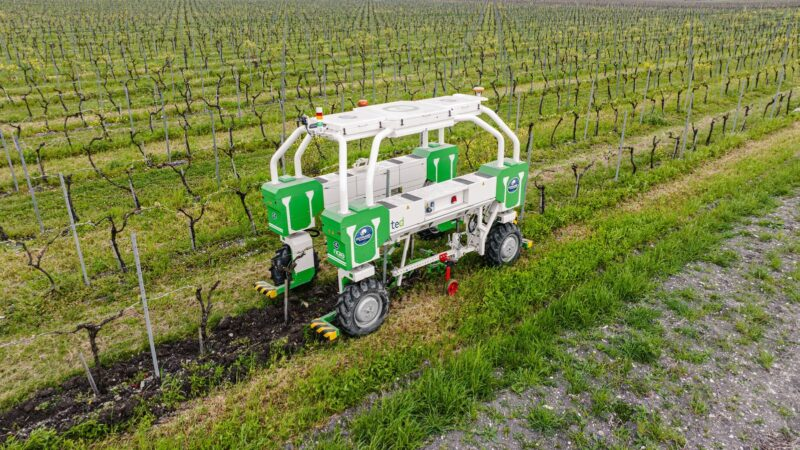
\includegraphics[width=0.4\textwidth]{figures/intro/agricultura.jpg}
        \caption{Robot de limpieza de viñedos de la empresa Naio Technologies}
        \label{fig:agricultura}
    \end{figure}

    \item \textbf{Conducción Autónoma:} los vehículos autónomos están equipados con sistemas avanzados de detección, procesamiento de datos y actuadores. Estos son capaces de navegar en el tráfico sin necesidad de intervención humana en la mayoría de escenarios, lo que los sitúa en el nivel 3 en la escala J3016. Su desarrollo tiene como objetivo mejorar la seguridad vial, aumentar la eficiencia del transporte y facilitar la movilidad de personas con diversidad funcional. Diversas empresas como Tesla, AutoX o Waymo (\ref{fig:autoX}) ya ofrecen servicios comerciales.
    \begin{figure}[H]
        \centering
        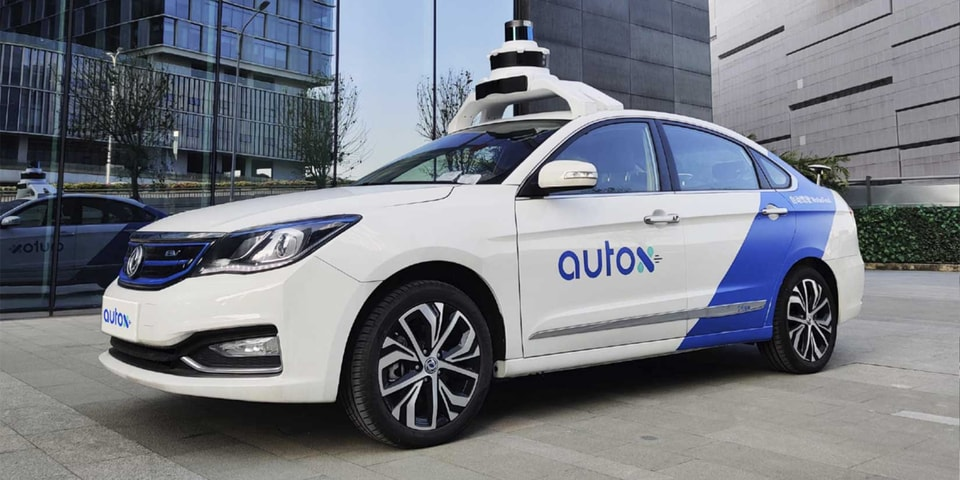
\includegraphics[width=0.4\textwidth]{figures/intro/autoX.jpg}
        \caption{Taxi autónomo de la empresa AutoX}
        \label{fig:autoX}
    \end{figure}

    % \item \textbf{Inspección y mantenimiento:} los robots, tanto drones como robots cuadrúpedos, realizan de forma más eficiente y segura la inspección de entornos de difícil acceso o de gran superficie. Están equipados de sensores que suelen ser cámaras o LIDARs y algoritmos que componen todos los datos tomados en un solo modelo para su posterior análisis que puede ser de forma automática o manual.  \ref{fig:inspección}
    % \begin{figure}[H]
    %     \centering
    %     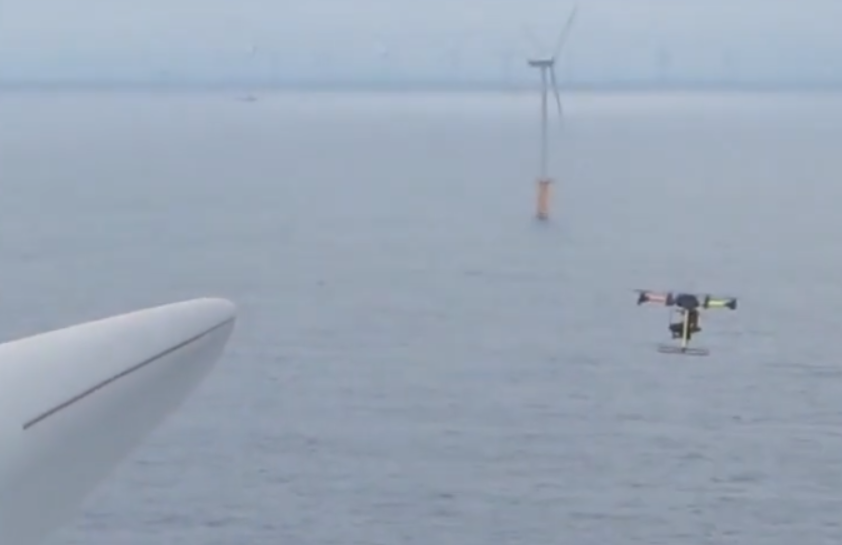
\includegraphics[width=0.6\textwidth]{figures/intro/drone.png}
    %     \caption{Robot de inspección de aerogeneradores de la empresa Helvetis}
    %     \label{fig:inspección}
    % \end{figure}

    \item \textbf{Logística:} los robots son más eficientes que los humanos a la hora de transportar las mercancías entre distintos puntos de las instalaciones, ya que son capaces de realizarlo de forma autónoma y constante durante un mayor periodo de tiempo. Estos están equipados con sistemas de navegación avanzados y con sensores destinados a disminuir la posibilidad de fallo. \ref{fig:almacenes}
    \begin{figure}[H]
        \centering
        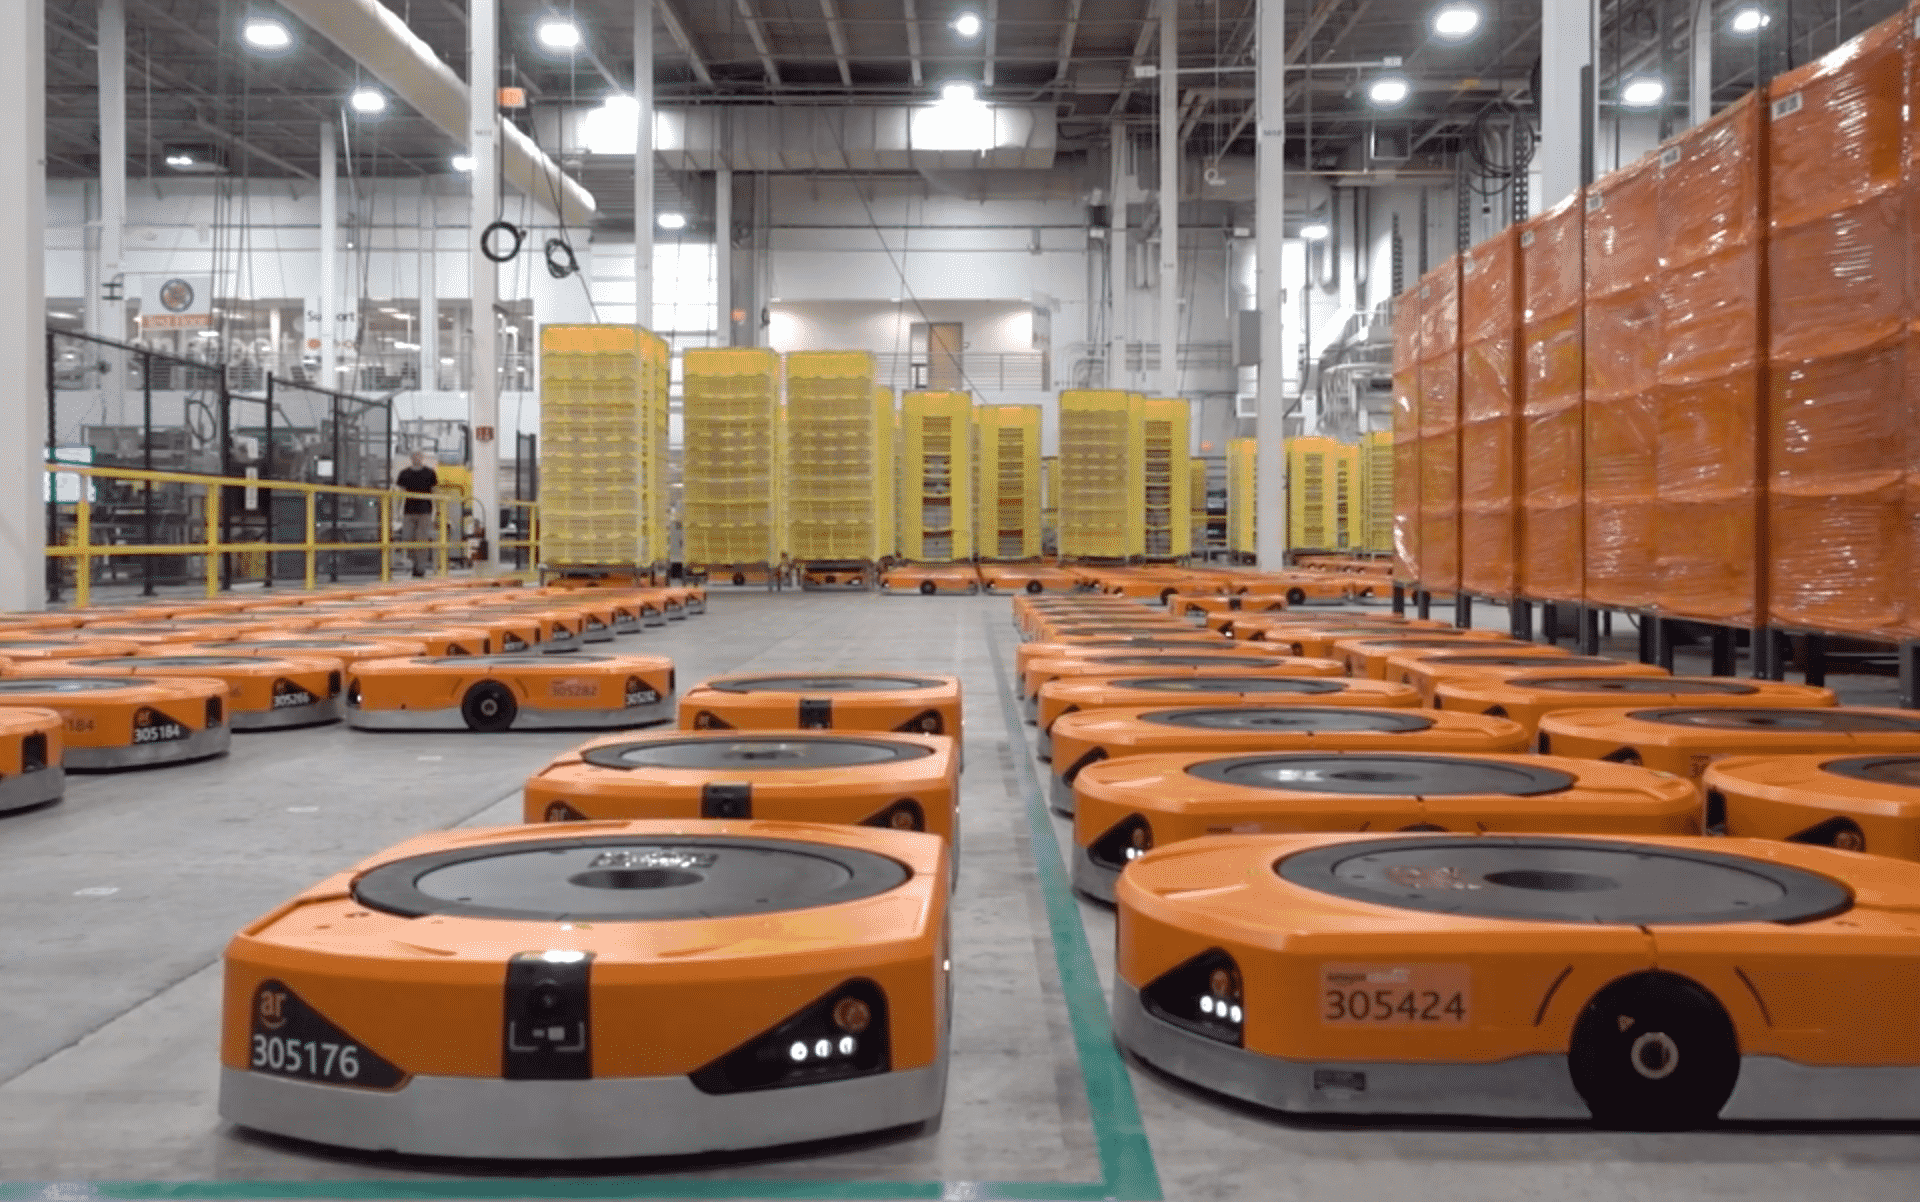
\includegraphics[width=0.4\textwidth]{figures/intro/amazon.png}
        \caption{Robots empleados en los almacenes de Amazon}
        \label{fig:almacenes}
    \end{figure}

    \item \textbf{Robots de Limpieza:} se encargan de la limpieza de diversos entornos, desde hogares hasta espacios públicos y oficinas, de forma autónoma usando algoritmos para planificar rutas de limpieza de manera eficiente. Incorporan sensores para detectar suciedad y obstáculos. \ref{fig:roomba}
    \begin{figure}[H]
        \centering
        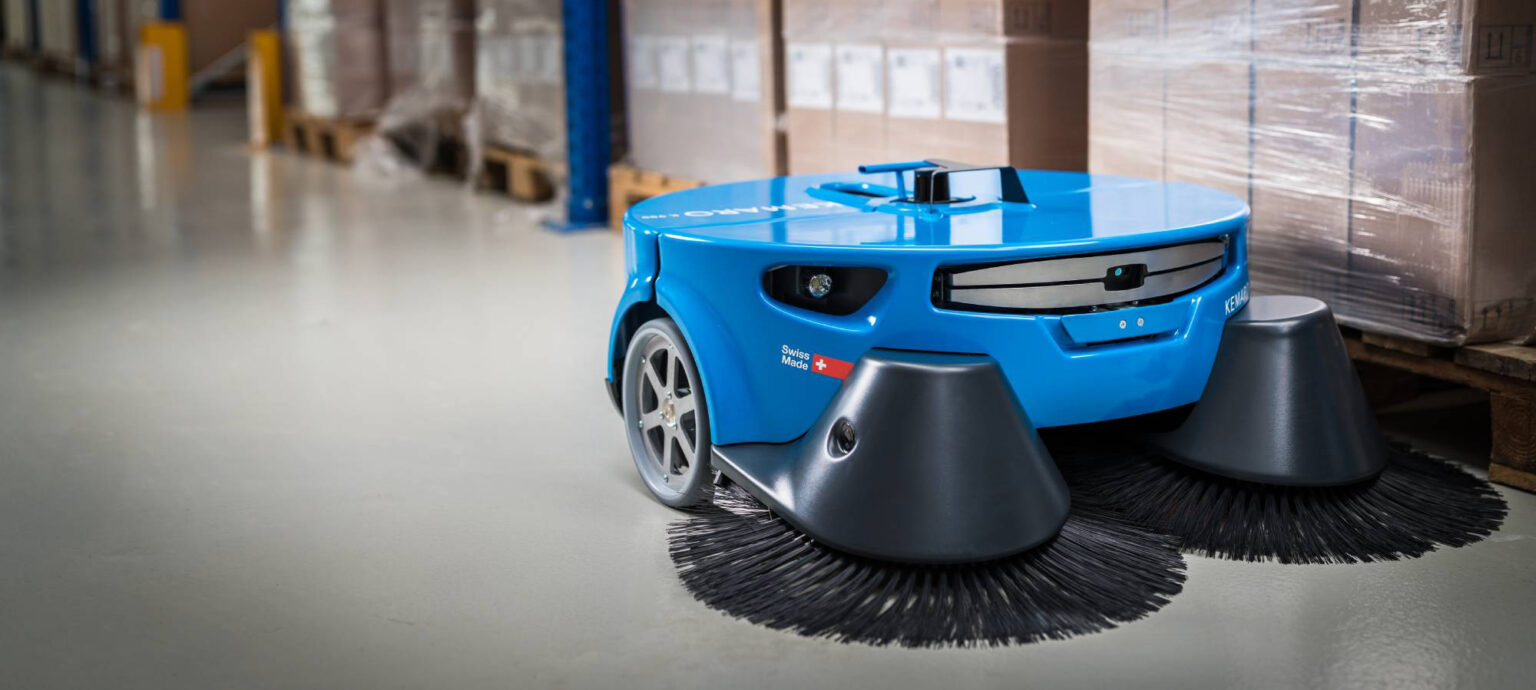
\includegraphics[width=0.5\textwidth]{figures/intro/vacuum.jpeg}
        \caption{Robot de limpieza industrial K900 de la empresa Kemaro}
        \label{fig:roomba}
    \end{figure}
    
\end{itemize}


\subsection{Desarrollo de aplicaciones robóticas}

Las aplicaciones robóticas han ido ganando complejidad para igualar a los avances en inteligencia artificial y en el desarrollo de componentes \textit{hardware}. La arquitectura software más utilizada actualmente en las aplicaciones robóticas es la de varios nodos distribuidos que ejecutan de forma paralela a distintos ritmos y que requieren de información variada para su funcionamiento. Este método es capaz de combinar las necesidades que requieren las aplicaciones robóticas, que son la reactividad para reaccionar e interaccionar con su entorno, y la toma de decisiones complejas y deliberadas. Con el fin de ayudar al desarrollo de aplicaciones robóticas han aparecido los \textit{middlewares} robóticos y los simuladores.

Los \textit{middlewares} robóticos ofrecen una abstracción del hardware y de las bibliotecas de comunicaciones para facilitar el desarrollo de aplicaciones. Estos \textit{middlewares} también tienen soporte para distintos simuladores. El más extendido en el mundo de la robótica, mayormente en la robótica de servicios, es ROS 2, que se explicará detalladamente en la sección \ref{ros_2}. ROS 2 soporta el uso de nodos distribuidos y su comunicación para desarrollar aplicaciones complejas.

\begin{figure}[H]
    \centering
    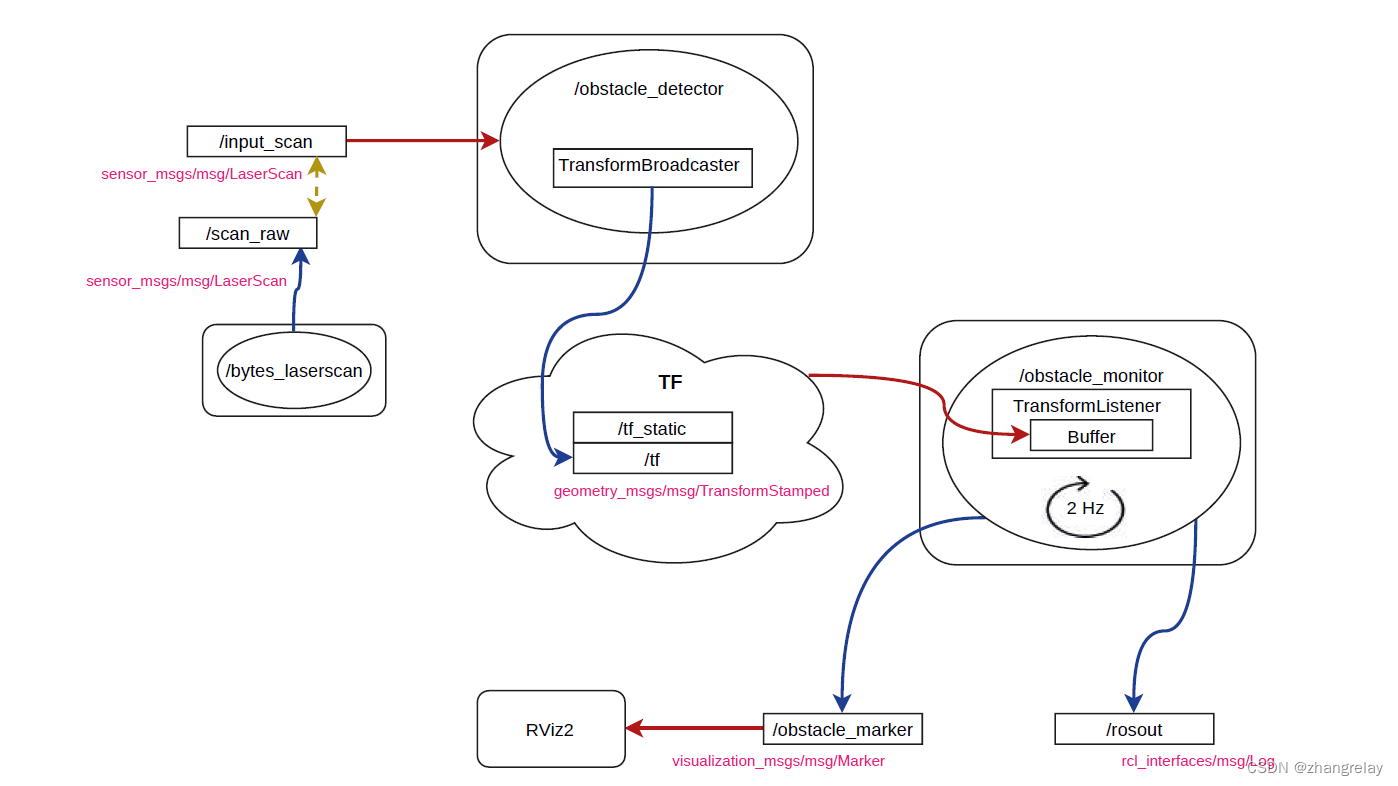
\includegraphics[width=0.7\textwidth]{figures/intro/c_graph.png}
    \caption{Grafo de nodos de una aplicación en ROS 2}
    \label{fig:ejemplo}
\end{figure}

Los simuladores permiten reproducir entornos físicos realistas para la depuración y ejecución de aplicaciones robóticas sin el riesgo de dañar equipos reales. Para ello, los simuladores tienen la capacidad de replicar distintos elementos físicos, como la gravedad, la colisión de objetos, la fricción, la luminosidad, etc. y ofrecen varios sensores y actuadores para su uso desde las aplicaciones robóticas. Todos estos elementos y parámetros son configurables, lo que permite simular de manera más detallada los diferentes mundos. Uno de los simuladores más utilizados es Gazebo (sección \ref{gazebo}), que cuenta con integración total con ROS 2.

\begin{figure}[H]
    \centering
    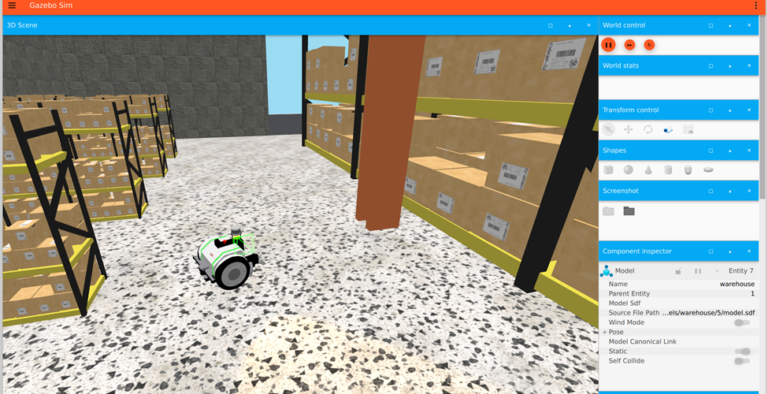
\includegraphics[width=0.6\textwidth]{figures/intro/gazebo.png}
    \caption{Entorno simulado en Gazebo}
    \label{fig:ejemplo}
\end{figure}

\subsection{Paradigmas de las aplicaciones robóticas}

Los componentes usados en las aplicaciones robóticas tienen funciones heterogéneas, pero pueden ser normalmente clasificados en tres tipos de componentes: 

\begin{itemize}
    \item \textbf{Componentes reactivos:} proporcionan una respuesta rápida ante cambios en el entorno. Están basados en el principio de estímulo-respuesta, lo que permite al robot actuar de forma rápida ante cambios no previsibles, sin necesidad de usar algoritmos de planificación de mayor complejidad. Habitualmente estos componentes realizan tareas que se deben ejecutar de forma inmediata y con alta frecuencia, como esquivar obstáculos o seguir una ruta. 

    \item \textbf{Componentes deliberativos:} realizan tareas complejas que requieren de la deliberación previa de múltiples factores y consecuencias. Permiten la toma de decisiones basadas en modelos internos del mundo, planificación a largo plazo de acciones complejas o la resolución autónoma de problemas. Se encargan de un abanico de acciones más amplio que los componentes reactivos, como la toma de decisiones, la navegación por entornos no conocidos o la coordinación de movimientos de brazos robóticos. Habitualmente estos componentes se ejecutan con una frecuencia menor y generan planes que ejecutarán los componentes reactivos.

    \item \textbf{Componentes de gestión de la ejecución:} proporcionan una forma de organizar y coordinar las acciones del robot, usando distintos estados. Hay de distintos tipos, pero los dos más usados son las FSM o máquinas de estado finito y los árboles de comportamiento. Las FSM permiten controlar la aplicación robótica dividiendo el comportamiento del robot en un número finito de estados, cuyas transiciones están definidas por un conjunto de reglas claras y deterministas. Por otra parte, los árboles de comportamiento proporcionan una abstracción de mayor nivel, lo que permite crear comportamientos más complejos y reutilizables. Estos últimos son los que más fuerza están ganando estos últimos años, ya que proporcionan una mayor sencillez de uso a la vez que permiten desarrollar aplicaciones más complejas, y también poseen de un mayor número de herramientas para facilitar su uso. Además estos facilitan la expansión de la aplicación.

\end{itemize}

\section{Tecnologías web}

\subsection{Estado del arte}

Las tecnologías web han sufrido una evolución exponencial en la última década, mejorando la experiencia de los usuarios y haciendo más eficientes, versátiles y accesibles las aplicaciones web. En el origen de Internet, las páginas web eran únicamente estáticas, creadas con HTML básico. Con el paso de los años se introdujo CSS, que permitió personalizar su estética, y JavaScript, que permitía conseguir interactividad en las páginas web. Esta última introducción conllevó la creación de diferentes \textit{frameworks} para la mejora del dinamismo y reactividad de las aplicaciones web, siguiendo cada uno de estos distintos paradigmas para su consecución. Los más usados hoy en día son React, Node.js, jQuery y Next.js.

\begin{figure}[H]
    \centering
    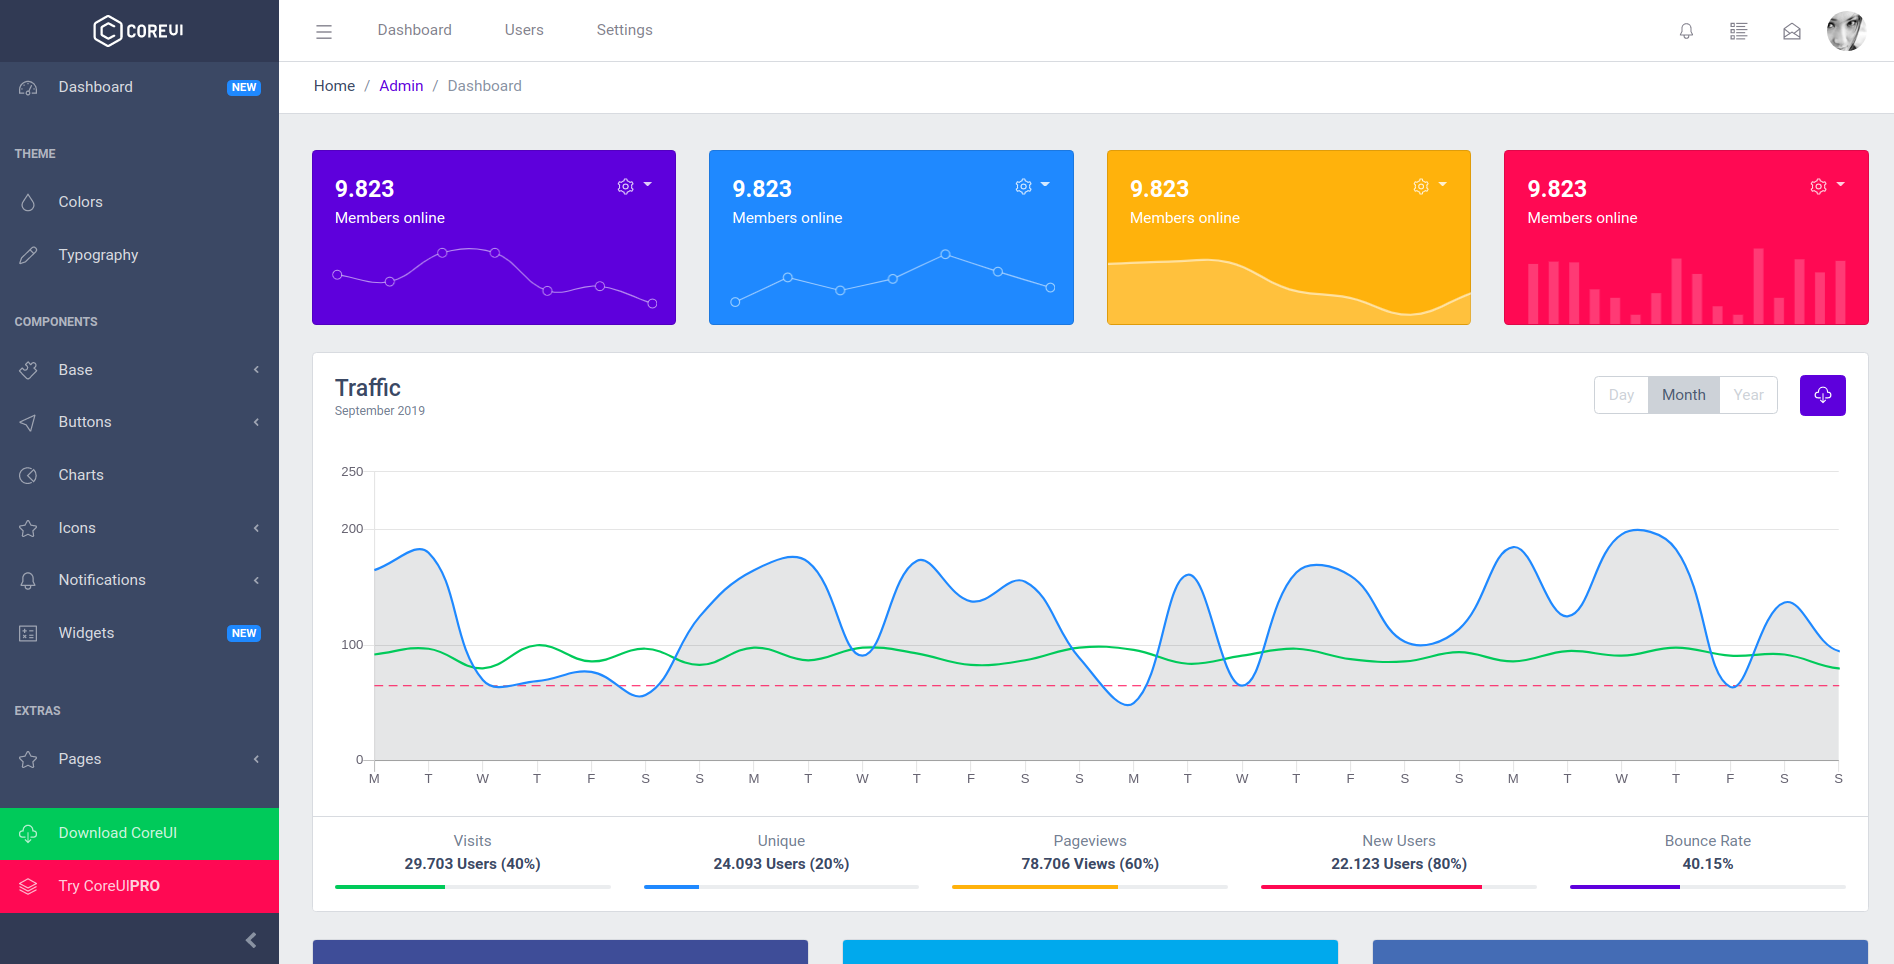
\includegraphics[width=0.6\textwidth]{figures/intro/react-ex.png}
    \caption{Interfaz creada con React}
    \label{fig:ejemplo}
\end{figure}

Por otra parte, también han evolucionado las tecnologías de bases de datos para satisfacer las necesidades de estas nuevas aplicaciones web. Las más populares son actualmente MySQL, PostgreSQL y MongoDB.

Algunos ejemplos de aplicaciones web modernas son:

\begin{itemize}
    \item \textbf{Plataformas de comercio electrónico}: estas permiten a los usuarios buscar, comparar y comprar productos con facilidad desde sus hogares. Utilizan tecnologías web avanzadas para ofrecer interfaces intuitivas y adecuadas al dispositivo de uso, así como procesos de pago seguros.

    \item \textbf{Aplicaciones de visualización de vídeos}: son aplicaciones web con elementos altamente reactivos, diseñada para transmitir contenido de video y audio a usuarios en todo el mundo. Estas utilizan tecnologías como WebRTC para proveer comunicación en tiempo real esencial para las videollamadas o el \textit{streaming}. 

\end{itemize}

\subsection{Plataformas web para programar}

En cuanto al ámbito de la programación, este también ha sufrido un gran auge en estos últimos años con la aparición de infinidad de plataformas o web IDEs creados para la educación o para el desarrollo profesional. Un par de ejemplos son las siguientes plataformas: 

\begin{itemize}

    \item \textbf{GitHub Codespaces\footnote{\url{https://github.com/features/codespaces}}}: ofrece un IDE donde los usuarios pueden escribir y desarrollar código en un entorno seguro integrado con GitHub. También permite compartir y probar código sin necesidad de configurar un entorno de desarrollo local.

    \item \textbf{Arduino Web IDE\footnote{\url{https://app.arduino.cc/}}}: permite desarrollar y cargar programas (\textit{sketches}) a placas Arduino directamente desde el navegador. Esta plataforma proporciona un IDE completo con todas las capacidades del IDE nativo como soporte para la edición de código, gestión de bibliotecas y acceso a una amplia gama de ejemplos.
    
\end{itemize}

\section{Plataformas web para la programación de aplicaciones robóticas}

La mezcla entre las tecnologías mencionadas anteriormente y la robótica da lugar a la aparición de plataformas web destinadas a la programación de aplicaciones robóticas desde el navegador. Para esto deben proporcionar adicionalmente un entorno para la simulación de la aplicación, algo que conlleva una mayor complejidad que la ejecución de código en los web IDE tradicionales. Estas plataformas se pueden dividir en dos dependiendo de la audiencia a la que vayan dirigidas:

\subsection{Plataformas educativas}

Aquellas enfocadas en el aprendizaje del desarrollo de aplicaciones robóticas o de conceptos relacionados con este ámbito. Las más conocidas a nivel internacional son: 

\begin{itemize}
    \item \textbf{TheConstruct\footnote{\url{https://app.theconstructsim.com/login/}}:} ofrece una amplia gama de cursos y simulaciones para aprender a programar robots usando ROS. La plataforma utiliza un IDE web y simuladores que corren en la nube, permitiendo a los usuarios desarrollar y probar sus aplicaciones y soluciones sobre robots simulados. Sus cursos abarcan todo tipo de niveles, cubriendo temas como la navegación, manipulación y percepción en entornos realistas. Figura \ref{fig:theconstruct}.

    \begin{figure}[H]
        \centering
        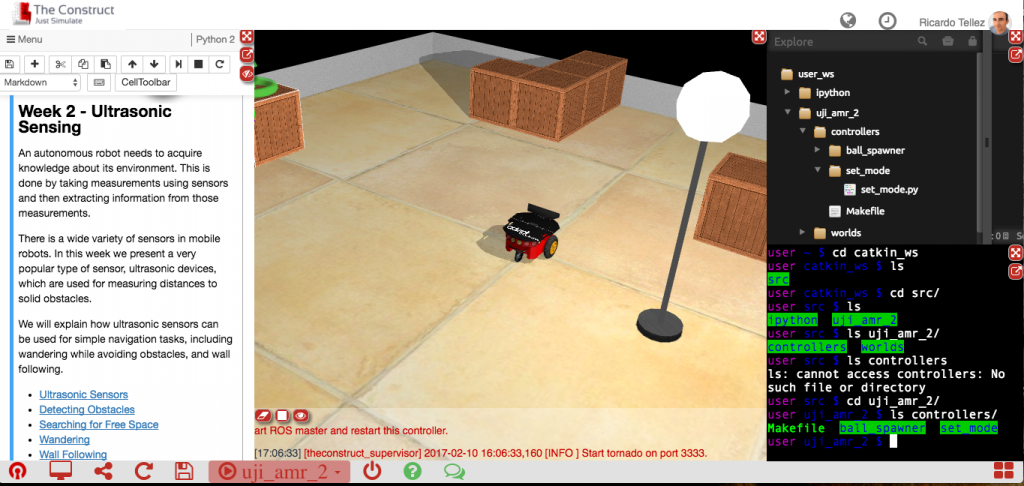
\includegraphics[width=0.7\textwidth]{figures/intro/theconstruct.png}
        \caption{Apariencia de TheConstruct}
        \label{fig:theconstruct}
    \end{figure}

    \item \textbf{Riders.ai\footnote{\url{https://riders.ai/en}}:} permite a los usuarios participar en competiciones de programación de robots, donde pueden medir sus habilidades contra las de otros programadores. A través de su IDE web, los participantes tienen la oportunidad de escribir, probar y optimizar su código en simulaciones que replican desafíos de robótica del mundo real. 
\end{itemize}

\subsection{Plataformas profesionales}

Estas tienen como propósito la programación y despliegue de soluciones robóticas en entornos de producción, ofreciendo una mayor gama de algoritmos y herramientas vanguardistas, dotando a la aplicación robótica de más complejidad y robustez que sus contrapartes educativas. Las dos plataformas más conocidas son:

\begin{itemize}
    \item \textbf{MoveitPro\footnote{\url{https://picknik.ai/pro/}}:} desarrollada por PickNik se centra en la programación de brazos robóticos en entornos no estructurados. Emplea árboles de comportamientos para la gestión de la ejecución de la aplicación, proporciona bloques predefinidos para tareas de planificación y percepción, entre otras funcionalidades como el uso de un simulador altamente realista (actúa como un gemelo digital) para facilitar la transición al brazo real. Está construido sobre la librería \textit{MoveIt}, estándar en la comunidad ROS 2 para la programación de brazos robóticos. 
    \item \textbf{Flowstate\footnote{\url{https://www.intrinsic.ai/flowstate/}}:} desarrollado por Intrinsic, una empresa propiedad de Google, y tiene como objetivo permitir la programación de aplicaciones industriales completas mediante un lenguaje de programación visual basado en bloques. Proporciona bibliotecas de bloques para tareas complejas y además, da a los usuarios la capacidad de expandirlas o crear las suyas propias. Por último, ofrece un entorno de simulación especializado, basado en ROS 2 y Gazebo.
    \item \textbf{Asimovo\footnote{\url{https://asimovo.com/}}:} plataforma de desarrollo de aplicaciones robóticas enfocadas en la robótica de servicio y proporciona una extensa colección de herramientas necesarias para el desarrollo de estas. Además, posee una \textit{biblioteca} de robots y de entornos de simulación. Figura \ref{fig:asimovo}.
    \begin{figure}[H]
        \centering
        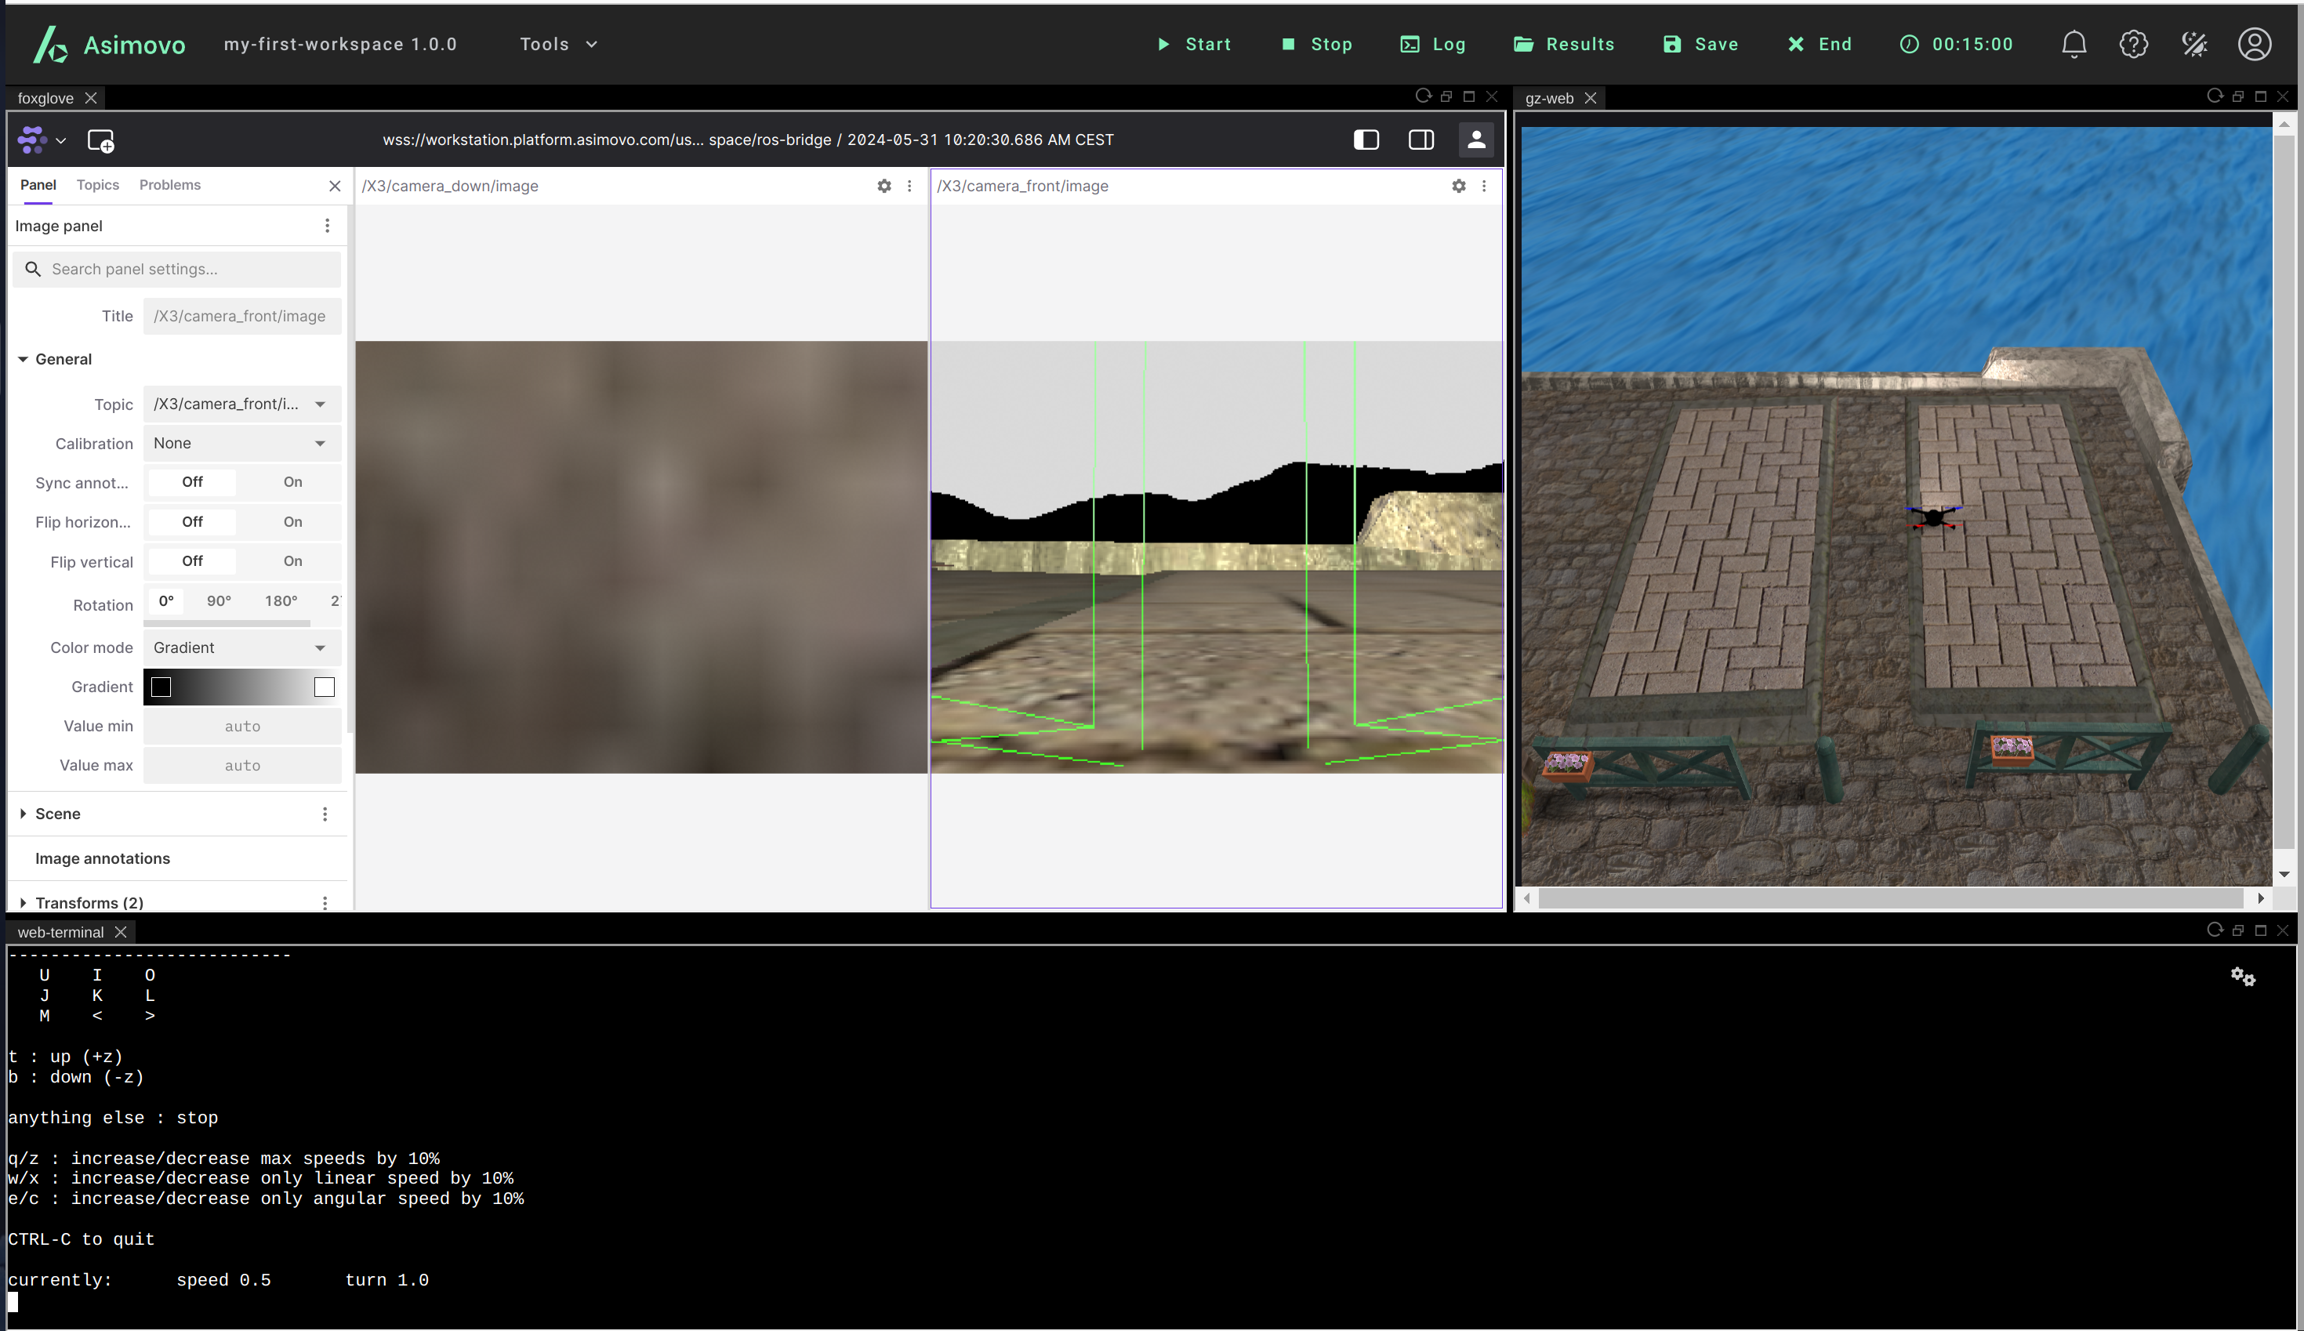
\includegraphics[width=0.7\textwidth]{figures/intro/asimovo.png}
        \caption{Apariencia de Asimovo}
        \label{fig:asimovo}
    \end{figure}
\end{itemize}

El objetivo principal de este TFG ha sido la mejora de BT Studio, una plataforma \textit{open source} que permite 
la programación de aplicaciones robóticas basadas en árboles de comportamiento desde un navegador web. 


    \chapter{Objetivos y metodología}\label{cap:planificación}

Ahora que ya se ha introducido el contexto y la motivación detrás de BT Studio, necesitamos establecer los objetivos que se van a desarrollar, así como la metodología a seguir.

\section{Objetivos}

El objetivo principal de este TFG es la mejora del IDE web robótico BT Studio, continuando con la filosofía \textit{open source} y con las bases que lo crearon. Este se puede dividir en los siguientes cinco subobjetivos, siendo el primero de ellos una combinación de múltiples más pequeños:  

\begin{enumerate}

    \item Mejora de los elementos del Frontend para mejorar la experiencia del usuario usando REACT y TS. 
  
    \item Adición de un monitor de ejecución en el editor de árboles de comportamiento para permitir tanto la visualización como la depuración sencilla de la aplicación robótica. 
  
    \item Integración con el Robotics Backend\footnote{\url{https://hub.docker.com/r/jderobot/robotics-backend}}, añadiendo la capacidad de ejecución de las aplicaciones desde el browser, usando un entorno dockerizado. 

    \item Integración en Unibotics \footnote{\url{https://unibotics.org/}} para facilitar su uso y hacer que el acceso a BT Studio sea más expandido y en línea. 
  
    \item Generación y mejora de aplicaciones de ejemplo para demostrar las capacidades de BT Studio mejorado. Se usará la integración con el Robotics Backend para su funcionamiento. Las aplicaciones serán \textit{Laser Bump and Go}, \textit{Follow Person} y  \textit{Receptionist}.
\end{enumerate}

El cumplimiento de cada uno de estos objetivos será detallado en el capítulo \ref{cap:validacion}.

\section{Metodología}

El modelo de trabajo de este TFG se basa en tres puntos principales:

\begin{itemize}
    \item \textbf{Reuniones semanales con los tutores}: gracias a esto y junto con la comunicación directa usando Slack se consigue un desarrollo ágil con un feedback rápido y detallado. 
    
    \item \textbf{Filosofía open source}: el trabajo se realizó íntegramente en múltiples repositorios de GitHub siendo los repositorios de BT Studio\footnote{\url{https://github.com/JdeRobot/bt-studio}}, Robotics Infrastructure\footnote{\url{https://github.com/JdeRobot/RoboticsInfrastructure}} y Robotics Application Manager\footnote{\url{https://github.com/JdeRobot/RoboticsApplicationManager}} públicos y el repositorio de Unibotics privado. Durante el proceso de desarrollo se trabajó con el método tradicional en estos entornos: incidencias, parches y versiones, facilitando el uso y la colaboración con otros desarrolladores. Se recibieron varias sugerencias y preguntas de varios desarrolladores. 
    
    La mentalidad \textit{open source}\footnote{\url{https://opensource.org/osd/}} es básica en el sector de la robótica como ha quedado demostrado con el éxito de ROS y ROS 2. Este TFG se adhiere estrictamente a esta mentalidad, estando este texto bajo la licencia Creative Commons Attribution-ShareAlike 4.0 International y todo el código asociado bajo GPLv3 a excepción de la integración con Unibotics que por otros motivos debe quedar en privado. También es importante resaltar que se ha interactuado en gran medida con la comunidad \textit{Open Source} con, por ejemplo, la participación en el evento internacional de FOSDEM 2025\footnote{\url{https://tinyurl.com/fosdemvideobtstudio}}. 

    \item \textbf{Hoja de ruta preciso}: el proyecto se desarrolló siguiendo un \textit{roadmap} claro y estructurado, organizado en distintas fases con objetivos específicos que estaban alineados con los subobjetivos explicados anteriormente. Se adoptó una metodología dinámica para guiar el desarrollo, lo que permitió una mayor flexibilidad y adaptación ante imprevistos. El trabajo se dividió en sprints coincidiendo con versiones oficiales nuevas de BT Studio, cada uno enfocado en la preparación e implementación de distintas funcionalidades y además en progresos semanales para obtener la realimentación del progreso de cada sprint. Este enfoque promovió una comunicación constante y efectiva con mis tutores y con los otros desarrolladores, permitiendo ajustes rápidos del plan y de los resultados obtenidos en cada sprint.
\end{itemize}

\section{Plan de trabajo}

El desarrollo de este Trabajo de Fin de Grado se ha producido entre marzo de 2024 y febrero de 2025. La introducción de subárboles pertenecientes a la versión 0.7 de BT Studio fueron realizados por otro desarrollador en el verano de 2024 como parte del GSOC\footnote{\url{https://theroboticsclub.github.io/gsoc2024-Oscar_Martinez/}} (Google Summer Of Code). 

\begin{enumerate}
    \item \textbf{Estudio de soluciones similares y estado del arte}.
    
    \item \textbf{Familiarización con tecnologías de desarrollo web}: principalmete Django, JS, TS, HTML, CSS y REACT. Estas tecnologías se usan de forma conjunta con otras del ámbito de la robótica, como Behavior Trees y ROS 2, y del ámbito de \textit{DevOps}, como Docker. Las características de cada tecnología y su uso en el TFG se detallan en el capítulo \ref{cap:tecnologias}.

    \item \textbf{Familiarización con el estado de BT Studio}: estudiar su funcionamiento y sus capacidades para ver posibles puntos de mejora y desarrollo.

    \item \textbf{Versión 0.4}: mejora de la interfaz de usuario y solución de problemas que perjudican la experiencia del usuario con de BT Studio.  
    \begin{itemize}
        \item Mejoras de la interfaz, añadiendo entre otras cosas modales personalizados en vez de los estándares del navegador.
        \item Creación de la aplicación de ejemplo Receptionist para su uso de forma local.
        \item Creación de una página web para la documentación de BT Studio.
        \item Solución de problemas de funcionamiento misceláneos.
        \item Creación de plantillas para las acciones.
    \end{itemize}

    \item \textbf{Versión 0.5}: mejora del editor visual de árboles de comportamiento.
    \begin{itemize}
        \item Personalización de las acciones en el editor visual de árboles de comportamiento.
        \item Añadir botones con funcionalidad adicional en el editor visual.
        \item Creación de modales para el cambio de universos.
    \end{itemize}

    \item \textbf{Versión 0.6}: mejoras en el control de ficheros e introducción del monitor de ejecución. 
    \begin{itemize}
        \item Creación de un explorador de ficheros con directorios plegables.
        \item Centralización y estandarización de los componentes de CSS.
        \item Creación del monitor de ejecución.
    \end{itemize}

    \item \textbf{Versión 0.7}: mejoras en el monitor de ejecución e introducción de subárboles.
    \begin{itemize}
        \item Introducción del uso de subárboles y la composición de árboles de comportamiento.
        \item Mejora de la personalización de acciones en el editor visual de árboles de comportamiento.
        \item Mejora del monitor de ejecución.
    \end{itemize}

    \item \textbf{Versión 0.7.1}: monitor de ejecución para subárboles y ejecución dockerizada.
    \begin{itemize}
        \item Introducción de la ejecución dockerizada de BT Studio al estilo de Robotics Academy\footnote{\url{https://github.com/JdeRobot/RoboticsAcademy}}.
        \item Introducción del soporte al Robotics Backend.
        \item Reintroducción de los universos personalizados.
        \item Mejora del monitor de ejecución para funcionar con subárboles.
    \end{itemize}

    \item \textbf{Versión 0.8}: solución de problemas e integración con Unibotics\footnote{\url{https://unibotics.org}}.
    \begin{itemize}
        \item Introducción de la barra de estado en la interfaz para controlar la conexión con el Robotics Backend.
        \item Solución de problemas en el guardado del estado del editor visual de árboles de comportamiento.
        \item Integración como submódulo de Unibotics.
    \end{itemize}

    \item \textbf{Versión 0.8.1}: migración a TS y cambio de editor.
    \begin{itemize}
        \item Creación de modales emergentes para mostrar errores, información o advertencias.
        \item Migración de todo el código que estaba escrito en JS a TS.
        \item Cambio del editor de texto de ACE\footnote{\url{https://github.com/ajaxorg/ace}} a Monaco\footnote{\url{https://github.com/microsoft/monaco-editor}}.
    \end{itemize}

    \item \textbf{Versión 0.8.2}: mejora del monitor de ejecución y mejora de documentación.
    \begin{itemize}
        \item Mejora de la documentación en la página web\footnote{\url{https://jderobot.github.io/bt-studio/documentation/}} con la creación de imágenes ilustrativas.
        \item Mejora de la implementación del monitor de ejecución.
    \end{itemize}

    \item \textbf{Versión 0.8.3}: división de los universos en mundos y robots.
    \begin{itemize}
        \item Introducción de más funciones del editor de texto Monaco, como autocompletado o resaltado sintáctico.
        \item División de los universos en mundos y robots.
    \end{itemize}

    \item \textbf{Aplicaciones robóticas de validación}: desarrollo de las tres aplicaciones de ejemplo propuestas, que permiten la validación de las versiones 0.7.1 en adelante. Para implementar las dos primeras soluciones me he basado en las ya existentes adaptándolas a las nuevas modificaciones que ha sufrido la herramienta. Por otra parte, para la última aplicación he utilizado paquetes externos complejos para demostrar su posible integración a las acciones de los árboles de comportamiento, así como un mayor número de nodos dentro del árbol para demostrar la escalabilidad de BT Studio, así como comprobar el correcto funcionamiento del monitor de ejecución. Estas aplicaciones están incluidas en el repositorio del proyecto para su consulta y uso. 
    
\end{enumerate}
    \chapter{Fundamentos técnicos}\label{cap:tecnologias}

En este capítulo se detallan los fundamentos técnicos detrás de las mejoras a BT Studio, es decir, todas las herramientas, tecnologías y librerías utilizadas para el desarrollo de estas. Dada la naturaleza de BT Studio, estas herramientas pertenecen únicamente al ámbito del software y están divididas generalmente en dos tipos: herramientas usadas para el desarrollo web y herramientas para el desarrollo robótico. La única excepción a esta separación es el lenguaje de programación Python, que se usa en ambos. 

\section{Lenguaje Python}

Python\footnote{\url{https://www.python.org/}} es un lenguaje de programación de alto nivel interpretado, orientado a objetos (aunque también permite programación funcional) y con semántica dinámica. Es utilizado en un gran número de aplicaciones, desde servidores web a inteligencia artificial. 
En de BT Studio se ha utilizado la versión 3.10.12. 

Entre sus características más destacadas podemos encontrar:

\begin{itemize}
    \item Sintaxis sencilla y legible que enfatiza la legibilidad y, por lo tanto, reduce el costo de mantenimiento del programa.
    \item \textit{Batteries included}\footnote{\url{https://peps.python.org/pep-0206/}}: contiene mucha funcionalidad adicional out-of-the-box incluida en su librería standard. Además, existen infinidad de librerías de terceros. 
    \item Su uso es gratuito y posee una licencia de código abierto. 
    \item \textit{Tipado dinámico}: no es necesario declarar el tipo de las variables al inicializarlas y este puede cambiar en función del valor de la variable en un determinado momento. También se pueden declarar los tipos para volverlo estricto.
    \item Es un lenguaje interpretado, por lo que no necesita compilar el código. Las sentencias del programa se ejecutan conforme se leen. 
\end{itemize}

Todas estas características conllevan un empeoramiento del rendimiento y consumo de memoria comparado con otros lenguajes como C, lo que restringe el tipo de sistemas que pueden usarlo. Esto en el caso de BT Studio no afecta, y además Python es requerido por los siguientes motivos:

\begin{itemize}
    \item El motor de ejecutor de árboles solo permite describir las acciones en Python.
    \item El Robotics Backend, entorno donde se ejecutan las aplicaciones, solo soporta Python. 
    \item El backend web de BT Studio utiliza el framework Django que usa Python. 
\end{itemize}

\section{Herramientas de desarrollo web}

Estas son las herramientas que han sido usadas para los cambios en el backend y el frontend web, así como en las que se basa BT Studio. Este primero tiene como función servir la página web del IDE y proveer distintos servicios a través de una API REST. El segundo sirve para mostrar la interfaz gráfica en el navegador e interaccionar con esta, pudiendo usar los servicios soportados por el backend.

Se recapitulan ahora las tecnologías más usadas en estas mejoras, así como la mención a varias librerías usadas en la sección de React.

\subsection{HTML}

HTML\footnote{\url{https://html.spec.whatwg.org/}} es un lenguaje de marcado estándar usado para definir la estructura de un documento web mediante etiquetas, que encapsulan las diferentes partes del contenido para darles una determinada apariencia o funcionalidad. Estos archivos no son ejecutables, si no que son leídos y representados por los navegadores web de forma transparente al usuario. 

Para este trabajo, se ha utilizado la última versión del \textit{living standard} de HTML\footnote{\url{https://developer.mozilla.org/en-US/docs/Glossary/HTML5}}. 

\subsection{CSS}

CSS\footnote{\url{https://www.w3.org/Style/CSS/}} es un lenguaje de hojas de estilo usado para especificar la presentación y el estilo de un documento escrito en un lenguaje de marcado como HTML o XML. El objetivo de CSS es permitir la separación de contenido y presentación, incluidos diseño, colores y fuentes en distintos ficheros, consiguiendo dividir la estructura, de la apariencia de la aplicación.

En BT Studio se ha usado la última versión disponible de CSS, 4.15.

\subsection{JavaScript}

JavaScript\footnote{\url{https://ecma-international.org/publications-and-standards/standards/ecma-262/}} es un lenguaje de programación de alto nivel interpretado, usado habitualmente para dotar de interactividad y dinamismo a las páginas web. Es un lenguaje no tipado, es decir, no se permite la definición del tipo de una variable. Junto con HTML y CSS forma el \textit{stack} básico en el desarrollo web.

En el desarrollo de este trabajo se empezó usando JavaScript, pero se acabó remplazando por TypeScript.

\begin{figure}[H]
    \centering
    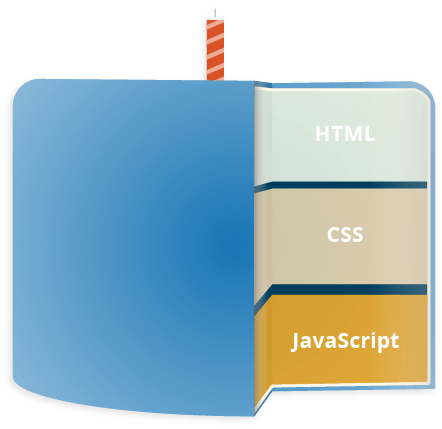
\includegraphics[width=0.3\textwidth]{figures/web_stack.png}
    \caption{Stack típico de desarrollo web}
    \label{fig:ejemplo}
\end{figure}

\subsection{TypeScript}
TypeScript\footnote{\url{https://www.typescriptlang.org}} es un lenguaje de programación de alto nivel basado en JavaScript, pero que cuenta con tipado estricto, es decir, se debe declarar el tipo de la variable al inicializarse y en todo lugar donde se pasen argumentos. Esto permite un mejor control del código, siendo completamente compatible con JavaScript

Concretamente, en el web IDE BT Studio se ha usado la versión 5.2.2 de TypeScript dentro de la librería REACT. 
\subsection{React}

React\footnote{\url{https://react.dev/reference/react}} es un \textit{framework} de JavaScript de código abierto diseñada para crear interfaces de usuario, especialmente en aplicaciones de una sola página. Es mantenida por Facebook y una comunidad de desarrolladores individuales y empresas. La versión empleada en este TFG fue la 18.2.0. 

Sus características más importantes son: 

\begin{itemize}
    \item \textbf{Componentes reutilizables}: permite la creación de interfaces de usuario a partir de piezas individuales llamados componentes. Estos mejoran la modularidad y escalabilidad de la aplicación.
    
    \item \textbf{Virtual DOM}: utiliza un DOM virtual que es una representación en memoria del DOM real con el objetivo de optimizar la actualización del este, actualizando solo las partes que han cambiado en cada momento, mejorando el rendimiento.
    
    \item \textbf{JSX o TSX}: introduce una sintaxis que permite escribir la estructura del componente de UI en código similar a HTML dentro de archivos JavaScript o TypeScript. Esto mejora la legibilidad del código y facilita el desarrollo. 
    
    \item \textbf{Flujo de datos unidireccional}: los datos solo se actualizan en un sentido, facilitando el rastreo de cambios a lo largo de la aplicación y mejora la predictibilidad y la facilidad de depuración.
    
    \item \textbf{Hooks}: son funciones que permiten a los componentes funcionales tener estado y acceder a características del ciclo de vida de React.
    
    \item \textbf{Ecosistema extenso}: al ser una librería de JavaScript existe un amplio ecosistema de herramientas, bibliotecas y frameworks compatibles con React.
\end{itemize}

React se ha utilizado para la creación de nuevos componentes en el frontend de BT Studio, así como en los ya existentes.

Algunas de las librerías compatibles con React más importantes durante el desarrollo de las mejoras han sido:

\begin{itemize}
    \item \textbf{Projectstorm React Diagrams}: usado tanto en el editor de árboles de comportamiento como en el monitor de ejecución. Más detalles de su uso en BT Studio, se pueden encontrar en este TFG \cite{TFG_BT_Studio}.
    \item \textbf{Monaco Editor\footnote{\url{https://microsoft.github.io/monaco-editor/}}}: usado para sustituir al antiguo editor ACE. Esta librería está mantenida por Microsoft bajo la licencia de código abierto MIT y proporciona un editor con toda la funcionalidad del usado en VS Code.
\end{itemize}

\subsection{Webpack}

Webpack\footnote{\url{https://webpack.js.org}} es una herramienta de código abierto usada para empaquetar aplicaciones de JavaScript junto con recursos del frontend como HTML, CSS o imágenes usando cargadores configurables.

En este TFG se ha usado Webpack en la integración de BT Studio en Unibotics y en la dockerización de la ejecución del primero.   

\subsection{Django}

Django\footnote{\url{https://www.djangoproject.com/}} es un \textit{framework} de desarrollo web de código abierto, gratuito y escrito en Python. Proporciona una estructura de organización específica siguiendo la filosofía de reducir la redundancia de código, lo que facilita la creación aplicaciones web complejas y robustas de manera eficiente. Para el desarrollo de BT Studio se ha utilizado la versión LTS, Django 4.2. 

\noindent Las características más importantes de Django en su uso en BT Studio son:

\begin{itemize}
    % \item \textbf{Rapidez}: fue diseñado para crear aplicaciones web lo más rápido posible. Esto implica que tiene un diseño claro, bien estructurado y con una gran variedad de funcionalidades y herramientas adicionales. 
    
    \item \textbf{Seguridad}: incluye herramientas para evitar los problemas comunes de seguridad, como los ataques XSS, el CSRF o la inyección SQL. Además, soporta de manera completa el protocolo HTTPS. Esto era necesario para permitir una integración en Unibotics segura. 
    
    % \item \textbf{Escalable}: una vez implementada una funcionalidad en Django, esta puede ser usada desde el nivel de prototipo hasta el despliegue en aplicación web con miles de usuarios con cambios mínimos. Esto lo consigue mediante herramientas como cachés o la división de bases de datos en particiones. 
    
    \item \textbf{Plantillas}: son archivos HTML enriquecidos con marcadores y etiquetas especiales de Django, que permiten la generación dinámica de la apariencia de la interfaz. 
    
    \item \textbf{Patrón modelo-vista-controlador}: es un patrón de diseño de software usado comúnmente para la implementación de interfaces y su lógica de control. Esto permite separar la lógica de la visualización. 
    \begin{itemize}
        \item \textit{Modelo}: representa los datos necesarios para una determinada aplicación y la estructura de la base de datos. 
        \item \textit{Vista}: define cómo se muestran los datos de la aplicación, así como la interfaz para realizar operaciones sobre ellos. 
        \item \textit{Controlador}: contiene la lógica para actualizar los modelos y las vistas en respuesta a las acciones de los usuarios. 
    \end{itemize}

    \item \textbf{Fácil mantenimiento}: al utilizar el patrón MVC y plantillas, la estructura resultante es modular y fácilmente reutilizable.
    
\end{itemize}

\begin{figure}[htp]
    \centering
    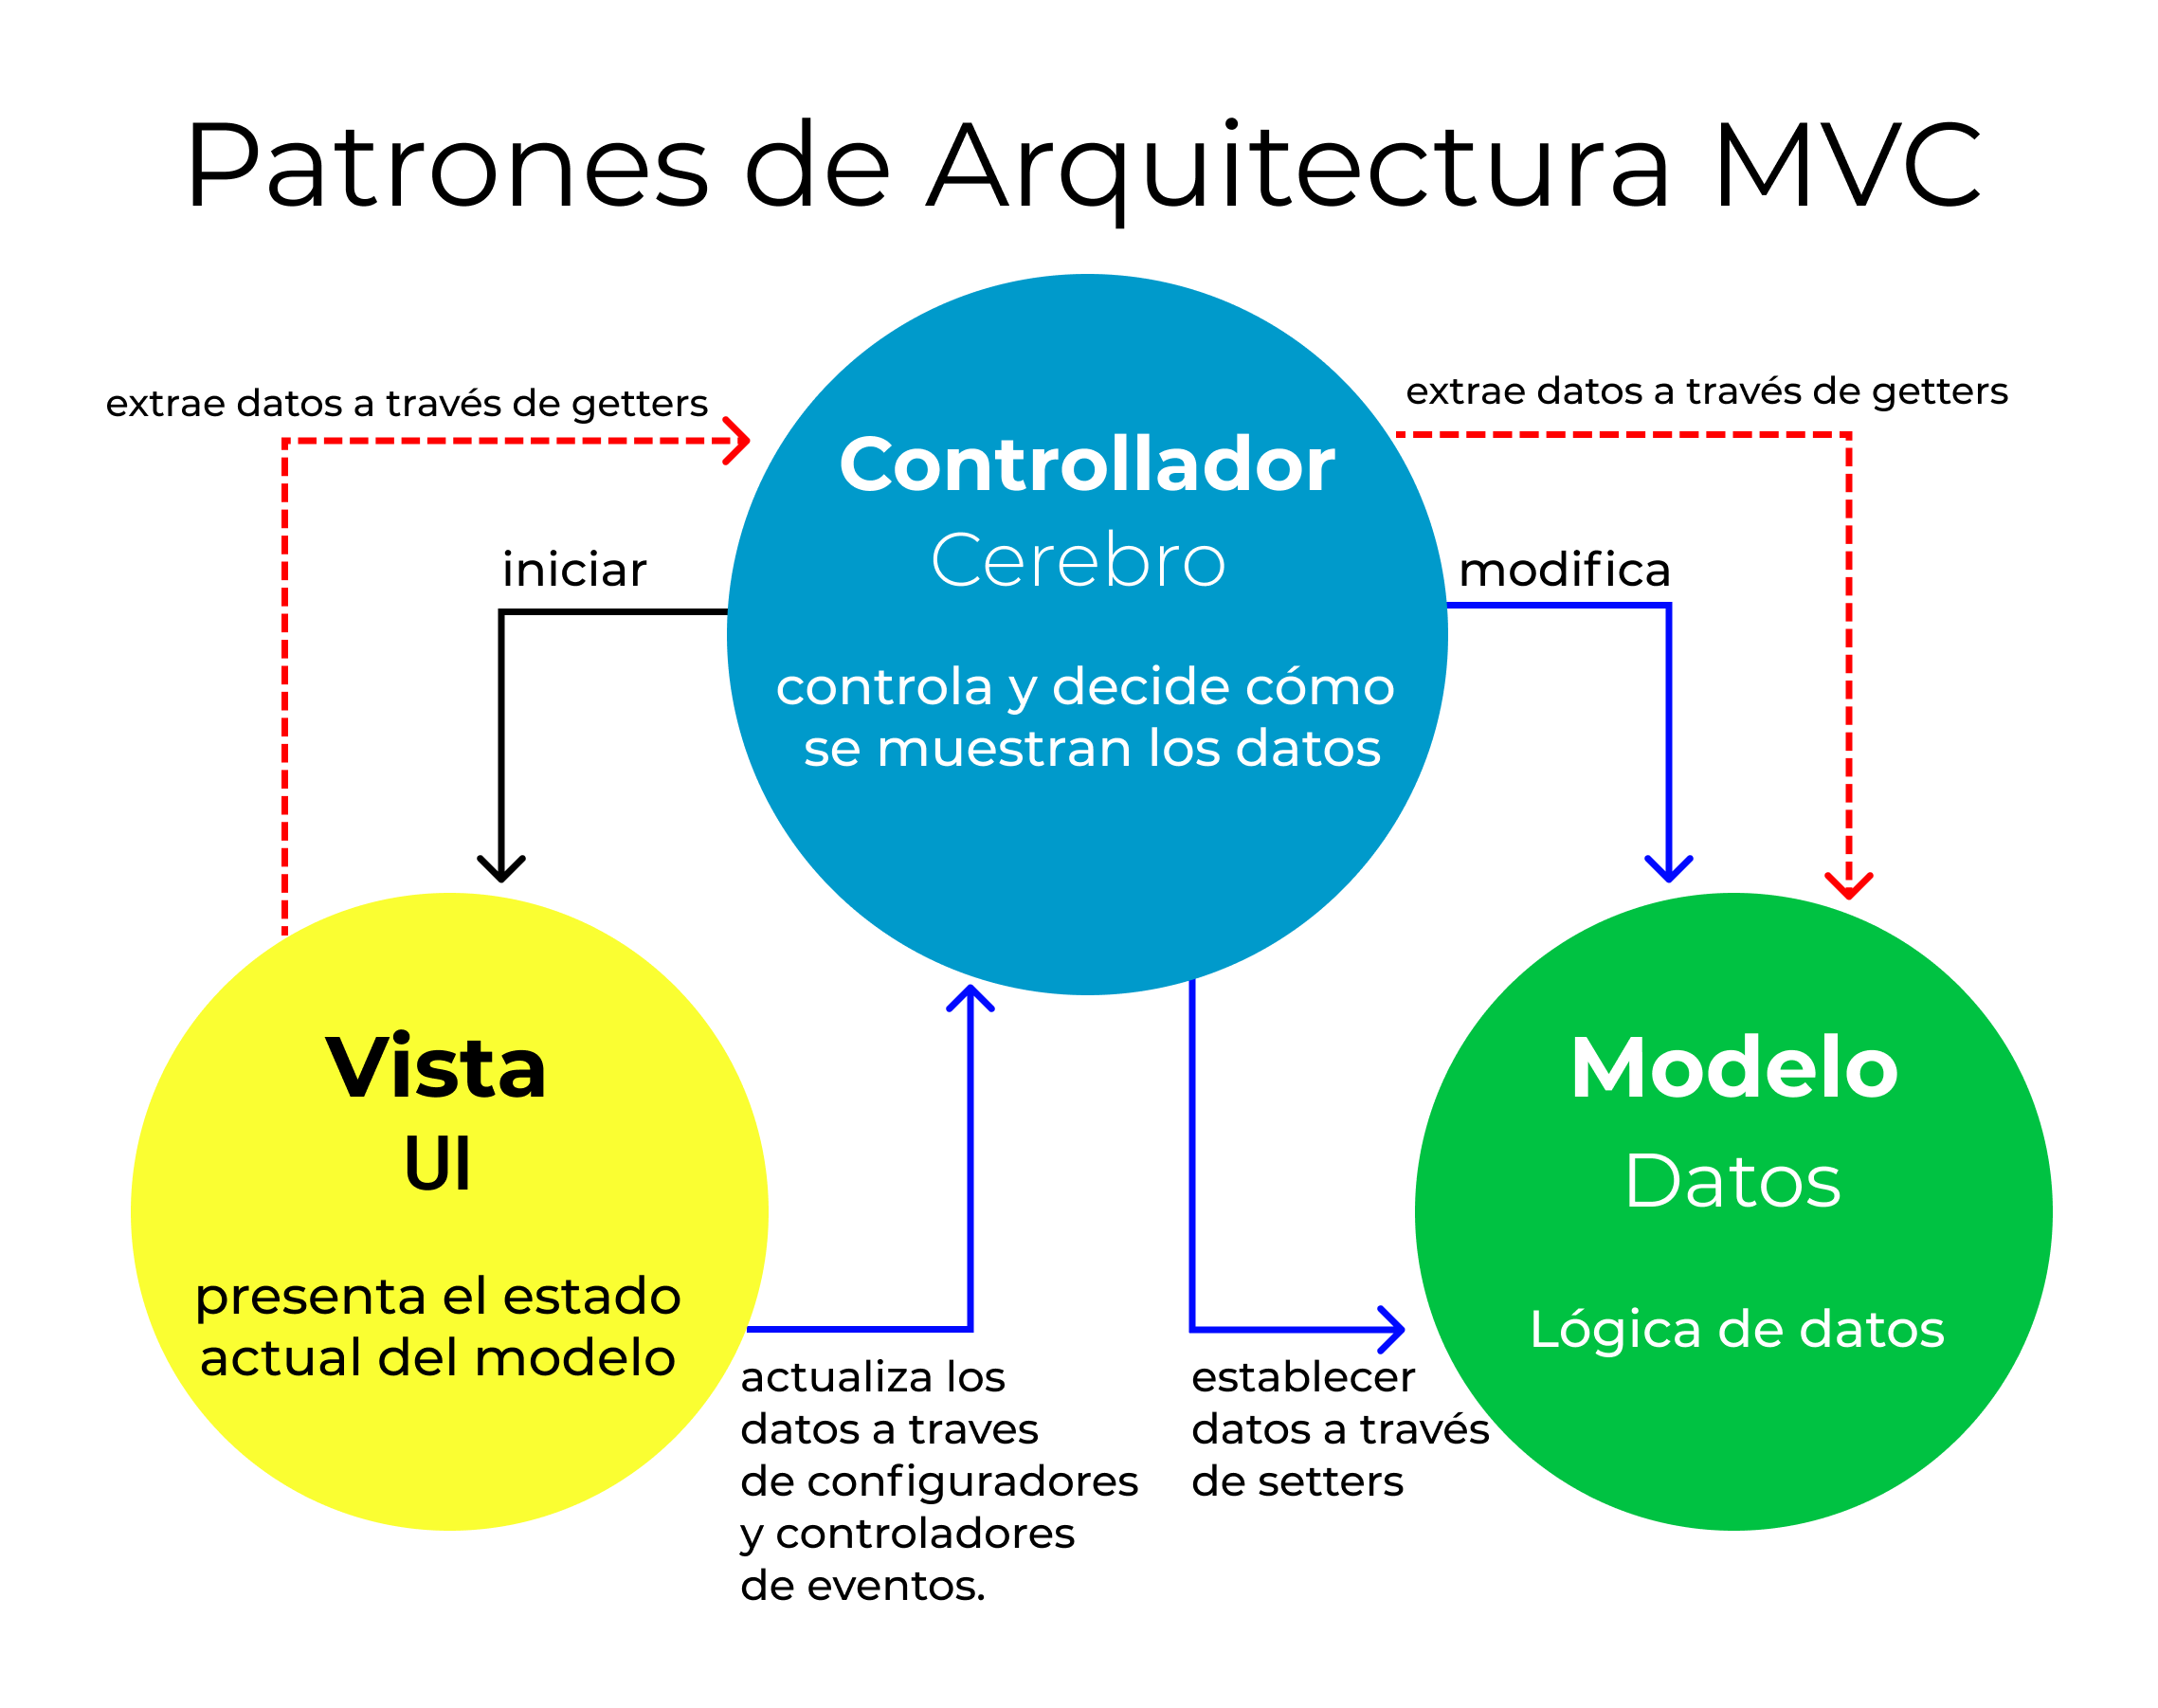
\includegraphics[width=0.6\textwidth]{figures/mvc.png}
    \caption{Esquema Modelo-Vista-Controlador}
    \label{fig:ejemplo}
\end{figure}

\subsection{WebSocket}

WebSocket\footnote{\url{https://www.rfc-editor.org/rfc/rfc6455}} es un protocolo de comunicación full-duplex sobre una única conexión TCP. Este protocolo tiene como objetivo el facilitar la interacción en tiempo real entre el cliente y el servidor, siendo fundamental para aplicaciones que requieren una comunicación bidireccional persistente y con baja latencia. En BT Studio, son usados para la comunicación entre el web IDE y el entorno de ejecución dockerizado. 

Las características más importantes de este protocolo son las siguientes:

\begin{itemize}
    \item \textbf{Comunicación Full-Duplex:} permite que tanto el cliente como el servidor envíen datos simultáneamente y en cualquier momento. Esto mejora la interactividad y el rendimiento de las aplicaciones al eliminar la necesidad de realizar múltiples conexiones HTTP para la comunicación.
    
    \item \textbf{Sesión persistente:} a diferencia del modelo de solicitud-respuesta utilizado en HTTP, WebSockets establece una conexión persistente que permanece abierta hasta que el cliente o el servidor desee.
    
    \item \textbf{Menor sobrecarga:} tras el establecimiento inicial de la conexión, la sobrecarga de datos es significativamente menor en comparación con HTTP, ya que los encabezados no necesitan ser enviados junto a cada mensaje.
    
    \item \textbf{Compatibilidad con navegadores:} el protocolo está soportado por todos los navegadores modernos.
    
    \item \textbf{Facilidad de uso:} la API de WebSockets es simple y fácil de usar, permitiendo establecer una comunicación bidireccional cliente-servidor con pocas líneas de código.
\end{itemize}

\subsection{VNC en la web}

Virtual Network Computing\footnote{\url{https://quentinsf.com/publications/virtual-network-computing/vnc-ieee.pdf}} es un sistema que permite la visualización y control remoto de una máquina, servidor, desde otra, cliente. En BT Studio se utiliza para transmitir la interfaz gráfica del simulador y el terminal que se encuentran dentro del docker del Robotics Backend, así como para permitir la interacción con ambas desde el frontend del web IDE donde se hallan dos clientes de VNC.

Las características fundamentales de VNC en una implementación web incluyen:

\begin{itemize}
    \item \textbf{Seguridad:} las implementaciones web de VNC pueden usar protocolos de seguridad como TLS/SSL para cifrar la conexión entre el navegador y el servidor VNC. 
    
    \item \textbf{Navegador como cliente VNC:} utilizando otras tecnologías web como HTML y WebSockets, es posible la implementación del sistema VNC en los navegadores. Esto permite a los usuarios controlar sistemas remotos directamente desde el navegador sin necesidad de instalar clientes de VNC en su propio sistema. Esto permite la interoperabilidad entre sistemas operativos. 
    
    \item \textbf{Interactividad:} gracias al uso de WebSockets para una comunicación bidireccional eficiente, las implementaciones web de VNC ofrecen interactividad con una mínima latencia. Esto resulta fundamental para BT Studio debido a que por naturaleza las simulaciones robóticas son muy reactivas. 
\end{itemize}

\section{Herramientas de desarrollo robótico}

\subsection{ROS 2}
\label{ros_2}

ROS 2\footnote{\url{https://docs.ros.org/en/humble/index.html}} (Robot Operating System 2) es un conjunto de librerías y herramientas para el desarrollo de aplicaciones robóticas. Este además incluye una extensa colección de drivers y algoritmos del estado del arte. Se puede consultar su diseño en profundidad en \cite{Macenski_2022}. La versión utilizada en este TFG es la última versión LTS disponible a su comienzo, Humble Hawksbill. 

Las aplicaciones que se generan en BT Studio son aplicaciones ROS 2, con un nodo que posee la capacidad de interactuar con los drivers de los sensores y actuadores del robot usando una interfaz llamada \textit{topic}. 

Las características que definen el diseño de ROS 2 son las siguientes:

\begin{itemize}
    \item \textbf{Arquitectura distribuida:} utiliza un modelo de comunicación basado en DDS (Data Distribution Service) para la comunicación entre componentes en el sistema. Esto permite además el uso de políticas de calidades de servicio que garantizan unos requisitos concretos a las comunicaciones. 

    \item \textbf{Flexibilidad en la comunicación:} soporta múltiples patrones de comunicación, como publicador/suscriptor, servicios y acciones.

    \item \textbf{API homogénea en Python y C++}: la funcionalidad de ROS 2 se encuentra en la librería \textbf{rcl}, escrita en C. A partir de esta, se proporcionan APIs en lenguajes de alto nivel a través de librerías clientes, como \texttt{rclcpp} para C++ y \texttt{rclpy} para Python, que pueden ser usadas de manera simultánea para distintos componentes dentro de una misma aplicación robótica. 

    \item \textbf{Herramientas de desarrollo y depuración:} proporciona un extenso conjunto de herramientas para la depuración y visualización de sistemas robóticos, como Rviz2, para facilitar el desarrollo y la prueba de aplicaciones robóticas.
    
    \item \textbf{Soporte multiplataforma:} ROS 2 es compatible con varios sistemas operativos, incluyendo Linux (Ubuntu y RHEL), Mac OS, Windows y otros sistemas operativos en tiempo real, extendiendo así su uso en entornos robóticos diversos.
\end{itemize}

Con todas estas características podemos definir ROS 2 de manera más exacta como un \textit{middleware} que utiliza un mecanismo de publicador/subscriptor anónimo para la comunicación usando mensajes tipados entre distintos procesos o nodos. 

\subsubsection{Componentes básicos}

Por último, los componentes funcionales básicos que forman parte de ROS 2 son los siguientes:

\begin{itemize}
    \item \textbf{Nodos}: unidad de computación básica dentro del grafo de ROS. Usan una librería cliente (\textit{rclpy} o \textit{rclcpp}) para comunicarse con otros nodos que pueden estar en el mismo proceso, en otros o incluso en una máquina distinta.

    \item \textbf{Topics}: permiten conectar productores (publicadores) de datos con consumidores (subscriptores) a través de un canal de nombre común (topic). Además, poseen distintas calidades de servicio para la recepción de estos mensajes.

    \item \textbf{Interfaces:} definen las estructuras de los mensajes intercambiados entre los nodos mediante un lenguaje de definición de interfaces simplificado (IDL). 

    \item \textbf{Servicios:} son llamadas a procedimientos remotos, es decir, un nodo cliente puede invocar la ejecución de tareas y obtener un resultado por parte de un nodo servidor. Estos son normalmente de corta duración debido a que son bloqueantes para el nodo cliente. Si tienen una duración mayor se usan acciones.
    
    \item \textbf{Acciones:} son llamadas a procedimientos remotos de larga duración. Las acciones proporcionan \textit{feedback} mientras se están ejecutando y pueden ser canceladas en cualquier momento. 

    \item \textbf{Parámetros:} permiten la configuración de los nodos al iniciarse o en tiempo de ejecución sin cambios en el código fuente. En ROS 2, los parámetros están asociados a cada nodo y estos deben declarar todos los parámetros que aceptan junto con su tipo. 

    \item \textbf{Launch system:} tiene como objetivo automatizar el lanzamiento de múltiples nodos desde un solo comando. Permite definir cómo y cuándo ejecutar cada programa con una sintaxis común de ROS que facilita su reutilización. Esta sintaxis suele estar en Python, XML o YAML.
    
    \item \textbf{Descubrimiento de nodos}: es llevado a cabo de manera automática por el \textit{middleware} encargado de las comunicaciones en ROS2. Esto permite modificar el grafo añadiendo o eliminando nodos que pertenezcan al dominio de ROS de la aplicación.
    
\end{itemize}

\subsection{Simulador Gazebo}
\label{gazebo}

Gazebo\footnote{\url{https://gazebosim.org/home}} es un simulador 3D de código abierto mantenido por la Open Source Robotics Foundation utilizado ampliamente en el desarrollo de sistemas robóticos, específicamente en ROS2. Ofrece la capacidad de simular con precisión el funcionamiento de robots en entornos complejos y dinámicos. En BT Studio, más concretamente en el entorno de ejecución dockerizada Robotics Backend, se usa la última versión de Gazebo Classic, Gazebo 11, y la moderna, Gazebo Harmonic. 

Sus características más importantes son:

\begin{itemize}
    \item \textbf{Simulación realista:} utiliza motores de física avanzados como ODE (Open Dynamics Engine), Bullet o DART para proporcionar una simulación adecuada de fuerzas, colisiones y materiales. Esto permite simular robots y sistemas de control en entornos seguros y controlados que se asemejan al mundo real. 
    
    \item \textbf{Entornos ricos y personalizables:} permite la creación de entornos detallados con una amplia gama de objetos, texturas y condiciones de iluminación. Estos entornos son definidos en el formato SDF\footnote{\url{http://sdformat.org/}}, basado en XML. 
    
    \item \textbf{Librerías de sensores y actuadores:} proporciona una amplia variedad de modelos de sensores y actuadores que imitan de manera realista el comportamiento y las limitaciones de los modelos reales.
    
    \item \textbf{Interfaz gráfica y herramientas de usuario:} permite visualizar y manipular las simulaciones de manera gráfica, incluyendo la capacidad de controlar el tiempo de simulación, visualizar datos de sensores y editar en tiempo real objetos y entornos.
    
    \item \textbf{Integración con ROS 2:} se integra de manera completa con ROS 2, permitiendo a la aplicación de ROS 2 interactuar con la simulación como si fuera hardware real. 
\end{itemize}

\begin{figure}[H]
    \centering
    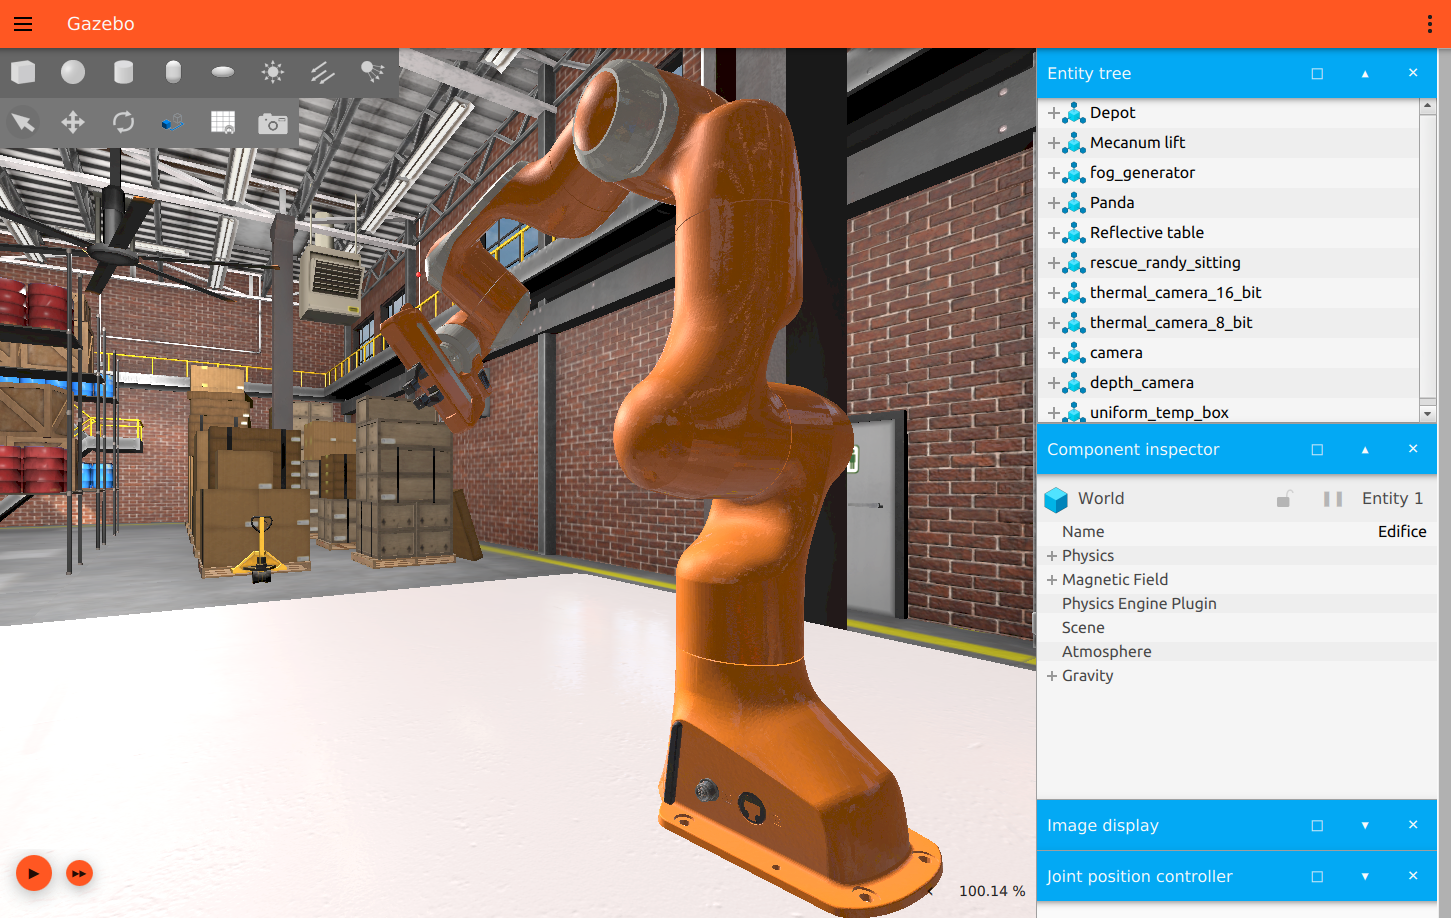
\includegraphics[width=0.8\textwidth]{figures/fundamentos/harmonic.png}
    \caption{Cliente gráfico de Gazebo Harmonic}
    \label{fig:ejemplo}
\end{figure}

\subsection{Árboles de comportamiento}

En esta sección se va a hablar de forma resumida sobre las características básicas de los árboles de comportamiento y de la librería PyTrees. Para una explicación más detallada sobre estos, BT.cpp y su uso en BT Studio se recomienda leer el TFG \cite{TFG_BT_Studio}.

\subsubsection{Definición}

Los árboles de comportamiento\cite{Colledanchise_2018} constituyen una manera de organizar la forma en la que un agente autónomo, ya sea un robot o una entidad virtual en un videojuego, alterna entre diferentes acciones. Para que una aplicación pueda usar este paradigma se necesita dividirla en distintos nodos reutilizables llamados acciones o nodos de control. Gracias a esto se consigue construir sistemas complejos que son al mismo tiempo modulares y reactivos.

\begin{figure}[H]
    \centering
    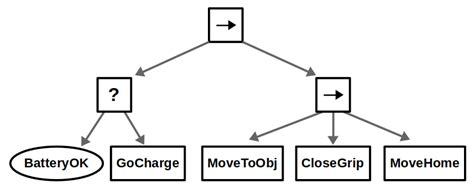
\includegraphics[width=0.8\textwidth]{figures/fundamentos/bt-example.png}
    \caption{Ejemplo básico de árbol de comportamiento}
    \label{fig:ejemplo}
\end{figure}

\subsubsection{Características}

Podemos entender la estructura de un árbol de comportamiento como la combinación de tres partes:

\begin{itemize}
    \item \textbf{Nodo raíz}: solo existe uno y es el origen del árbol de comportamiento. No tiene ningún nodo padre.
    \item \textbf{Nodos internos}: pueden existir cualquier número de estos y son los encargados de controlar el flujo de la ejecución. También son llamados nodos de control y poseen tanto un nodo padre como un número indefinido de nodos hijos.
    \item \textbf{Nodos externos}: pueden existir cualquier número de estos y son las acciones definidas por el usuario. Por esto también reciben el nombre de nodos de ejecución. Solo tienen un nodo padre.
\end{itemize}

La ejecución de un árbol de comportamiento empieza en el nodo raíz y se propagan a sus hijos usando señales a una determinada frecuencia llamadas \textit{ticks}. Cuando una de estas señales llega a un nodo hijo, este se ejecuta y devuelve uno de los siguientes estados: \textit{Running} si están ejecutando una tarea, \textit{Success} si ha conseguido su objetivo o \textit{Failure} en caso contrario. 

En la definición tradicional de los árboles de comportamientos, existen solo cuatro nodos de control de flujo (\textit{Sequence}, \textit{Fallback}, \textit{Parallel} y \textit{Decorator}) y dos de nodos de ejecución (\textit{Action} y \textit{Condition}). En BT.cpp\footnote{\url{https://github.com/BehaviorTree/BehaviorTree.CPP}}, la implementación de árboles de comportamiento en ROS 2, existen más nodos de control, pero no son importantes para este trabajo.

\noindent Funcionamiento de los nodos de control de flujo:

\begin{itemize}
    \item \textbf{Sequence:} ejecuta de manera secuencial sus hijos en el orden indicado hasta que uno devuelve \textit{Running} o \textit{Failure}. El nodo de control devolverá estos estados si esto ocurre o devolverá \textit{Success} si y sólo si todos los hijos lo devuelven.

    \begin{figure}[H]
        \centering
        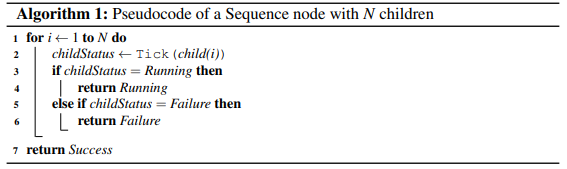
\includegraphics[width=0.8\textwidth]{figures/fundamentos/alg1.png}
        \caption{Algoritmo de un nodo tipo \textit{Sequence}}
        \label{fig:sequence}
    \end{figure}

    \item \textbf{Fallback:} ejecuta de manera secuencial sus hijos en el orden indicado hasta que uno devuelve \textit{Running} o \textit{Success}. El nodo de control devolverá estos estados si esto ocurre o devolverá \textit{Failure} si y sólo si todos los hijos lo devuelven.

    \begin{figure}[H]
        \centering
        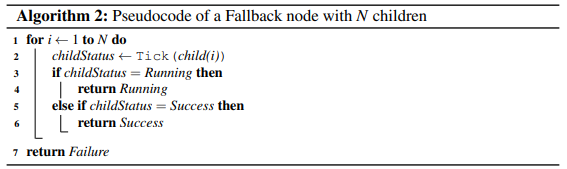
\includegraphics[width=0.8\textwidth]{figures/fundamentos/alg2.png}
        \caption{Algoritmo de un nodo tipo \textit{Fallback}}
        \label{fig:fallback}
    \end{figure}

    \item \textbf{Parallel:} ejecuta de manera paralela sus hijos y devolverá \textit{Success} si M hijos devuelven \textit{Success}, \textit{Failure} si N - M + 1 hijos devuelven \textit{Failure} y \textit{Running} en cualquier otro caso, siendo N es el número de hijos y M un umbral definido por el usuario.

    \begin{figure}[H]
        \centering
        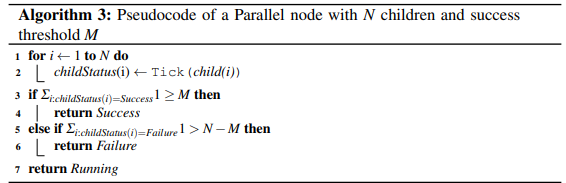
\includegraphics[width=0.8\textwidth]{figures/fundamentos/alg3.png}
        \caption{Algoritmo de un nodo tipo \textit{Parallel}}
        \label{fig:parallel}
    \end{figure}

    \item \textbf{Decorator:} son nodos de control que solo tienen un único hijo y manipulan el estado es la salida de este. Un ejemplo de este tipo es el nodo de control \textit{invert} que invierte la salida del hijo.

    \begin{figure}[H]
        \centering
        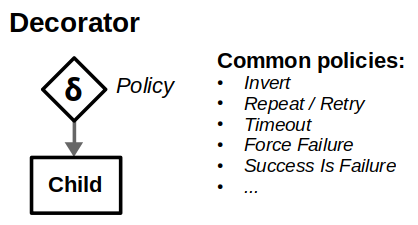
\includegraphics[width=0.4\textwidth]{figures/fundamentos/bt-decorator.png}
        \caption{Estructura de un nodo tipo \textit{Decorator}}
        \label{fig:parallel}
    \end{figure}
    
\end{itemize}

\noindent Funcionamiento de los nodos de ejecución:

\begin{itemize}
    \item \textbf{Action:} al recibir un tick, ejecutan una acción y devuelven \textit{Success} si ha tenido éxito, \textit{Failure} en caso contrario y \textit{Running} mientras está en ejecución. 

    \item \textbf{Condition:} al recibir un tick, comprueba una proposición y devuelve \textit{Success} o \textit{Failure} en función de su cumplimiento. Estos nodos nunca pueden devolver \textit{Running}.
    
\end{itemize}

\begin{figure}[H]
    \centering
    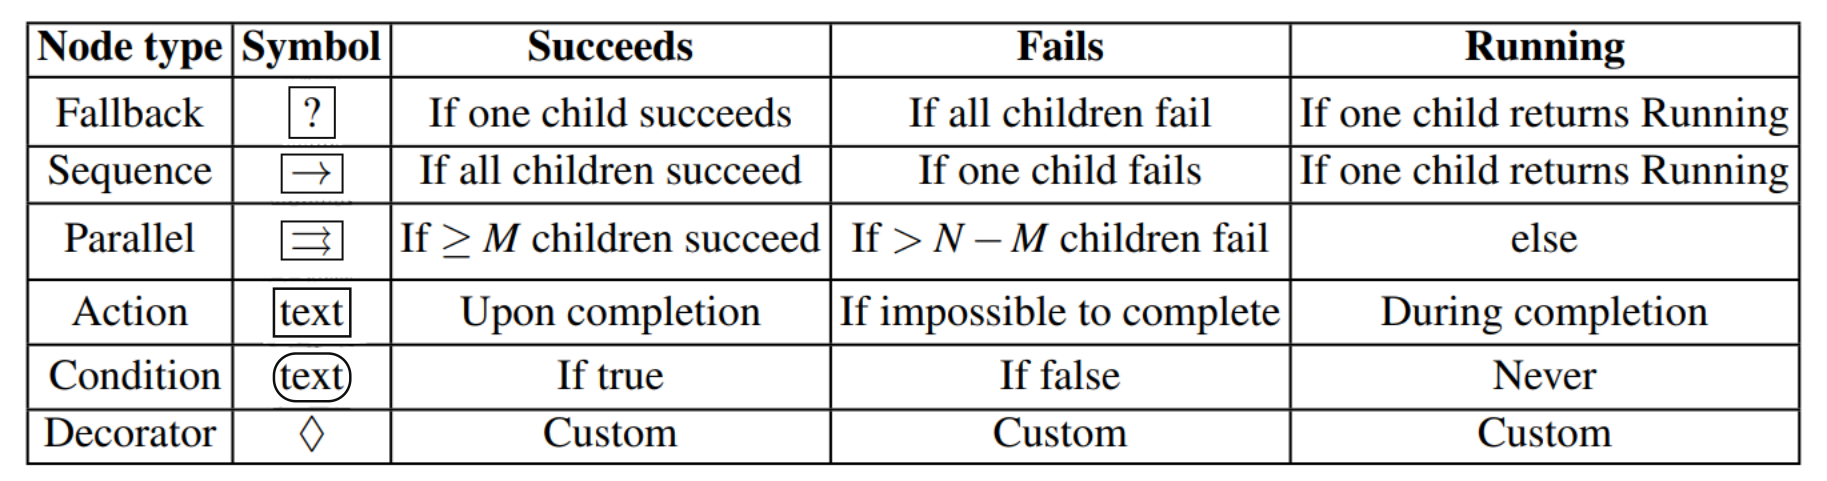
\includegraphics[width=\textwidth]{figures/fundamentos/node_types.png}
    \caption{Funcionamiento de los nodos de un árbol de comportamiento tradicional}
    \label{fig:ejemplo2}
\end{figure}

\subsubsection{PyTrees} \label{sec:blackboard}

PyTrees\footnote{\url{https://github.com/splintered-reality/py_trees}} es una librería para el desarrollo de árboles de comportamiento en Python en ROS 2. En BT Studio se usa la versión 2.3.0.

La característica que más importa para el desarrollo de este trabajo es la capacidad de extraer el estado del árbol de comportamiento en ejecución. Para una explicación más detallada sobre esta librería y su uso en BT Studio se recomienda la lectura del TFG \cite{TFG_BT_Studio}.

La extracción de este estado es posible gracias a las múltiple funciones encontradas en la sección de visualización de PyTrees, entre las que se encuentran:

\begin{itemize}
    \item \textbf{\textit{py\_trees.display.ascii\_tree()}}: devuelve el estado del árbol de comportamiento usando caracteres ASCII.
    \item \textbf{\textit{py\_trees.display.ascii\_blackboard()}}: devuelve el contenido de la \textit{blackboard} usando caracteres ASCII. La \textit{blackboard} es una memoria compartida que actúa como un diccionario de datos accesible por todos los nodos del árbol y permite la comunicación y el intercambio de información entre nodos mediante puertos.
\end{itemize}

A estas funciones es necesario pasarle como argumentos el árbol de comportamiento, pero como este ya era definido usando esta librería en BT Studio, no ha hecho falta utilizarla más que para lo indicado anteriormente.

% \subsubsection{Definición de nodos de ejecución}

% En PyTrees, los nodos de ejecución reciben el nombre de \textit{Behaviour} y no existe una separación explícita entre acciones y condiciones. Todos los comportamientos se implementan como una subclase de una clase base, donde se definen los siguientes métodos:

% \begin{itemize}

%     \item \textbf{\_\_init\_\_(name)}: inicialización mínima de la clase con la información necesaria para la introspección de los árboles mediante herramientas de depuración offline. 
    
%     \item \textbf{setup()}: método para inicialización diferida que se debe llamar manualmente o a través de métodos de la librería que configuran el comportamiento junto con sus descendientes. Adecuado para inicialización de hardware, middleware o cualquier configuración necesaria que no se desee en el constructor por interferir con la representación del árbol en gráficos o validaciones.
    
%     \item \textbf{initialise()}: invocado siempre que el estado anterior del comportamiento no sea \textit{RUNNING}. Aquí se realiza cualquier preparación requerida antes de comenzar la ejecución de una iteración del comportamiento. 
    
%     \item \textbf{update()}: este método se llama en cada tick del comportamiento. Dentro de este, se debe implementar la lógica principal del comportamiento, incluyendo decisiones, monitoreo o cualquier acción no bloqueante. Debe retornar un estado de \textit{py\_trees.common.Status}, que puede ser \textit{RUNNING}, \textit{SUCCESS}, o \textit{FAILURE}, basado en el resultado de la lógica implementada.
    
%     \item \textbf{terminate()}: se llama cuando el comportamiento cambia a un estado no activo (\textit{SUCCESS}, \textit{FAILURE} o \textit{INVALID}). Es útil para realizar limpieza o acciones finales al terminar o interrumpir el comportamiento.
% \end{itemize}

% Cada uno de estos métodos proporciona un punto de intervención en el ciclo de vida del comportamiento, permitiendo una implementación detallada y controlada de las acciones y condiciones dentro del árbol de comportamiento. Todas los nodos de ejecución de BT Studio se implementarán de esta manera. 

\subsection{Contenedores Docker}

Docker\footnote{\url{https://www.docker.com/}} es una plataforma que permite empaquetar una aplicación y sus dependencias en un contenedor virtual que puede ejecutarse en cualquier sistema operativo que lo soporte. Estos contenedores se pueden considerar como máquinas virtuales ligeras que virtualizan a nivel de sistema operativo.

Las características principales de Docker son:

\begin{itemize}
    \item \textbf{Portabilidad}: debido al uso de contenedores, se puede empaquetar la aplicación junto con sus dependencias dentro de los contenedores. Esto además asegura su ejecución consistente en diferentes entornos.
    
    \item \textbf{Aislamiento}: cada contenedor opera de manera aislada, mejorando así la seguridad y eliminando los conflictos entre aplicaciones.
    
    \item \textbf{Eficiencia}: utiliza los recursos del sistema operativo nativo de forma más eficiente que las máquinas virtuales tradicionales, lo que mejora su rendimiento y disminuye el consumo de recursos.
    
    \item \textbf{Gestión de imágenes}: usa imágenes para la creación de contenedores. Estas pueden tener control de versiones, ser almacenadas en repositorios y compartidas, facilitando la colaboración y la difusión. El repositorio de imágenes más usado es \textit{dockerhub}\footnote{\url{https://hub.docker.com}}.
    
    \item \textbf{Dockerfile}: archivo de texto que contiene todas las órdenes necesarias para construir una imagen Docker. Esto permite la automatización de la creación de imágenes de forma reproducible.
    
\end{itemize}

En este trabajo, el uso de Docker ha sido usado principalmente en el nuevo despliegue de BT Studio, la integración con el Robotics Backend y la integración en Unibotics.

\subsection{Unibotics}\label{sec:unibotics}

Unibotics\footnote{\url{https://unibotics.org/}} es una plataforma web para la programación de aplicaciones robóticas\cite{RoldanAlvarez2023} mantenida por la asociación de software libre JdeRobot\footnote{\url{https://jderobot.github.io/}}. Está dividida en tres secciones distintas: Academy, Games y BT Studio. Al comienzo de este trabajo solo la primera se encontraba funcional, y siendo la última añadida gracias a la labor realizada en este TFG. Además, Unibotics cuenta con tres despliegues diferentes para el testeo y desarrollo en esta:

\begin{itemize}
    \item \textbf{D1:} despliegue en la máquina local del desarrollador. Permite implementar y probar cambios de manera ágil, sin consecuencia de ningún tipo en caso de romper algún componente. 
    \item \textbf{D2:} despliegue en un servidor de pruebas, conectado a una granja reducida, donde se ejecutan las aplicaciones robóticas. Sirve para comprobar que los cambios funcionan en un entorno muy cercano al de producción.
    \item \textbf{D3:} despliegue en el entorno de producción, en la nube de cómputo AWS. Es al que pueden acceder los usuarios a través de la url del proyecto. 
\end{itemize}

Centrándonos en la parte de Academy, Unibotics proporciona un frontend web que permite la edición y ejecución de aplicaciones robóticas escritas en código Python desde el navegador para la resolución de ejercicios educativos predefinidos. Además, se ofrece un nivel superior de abstracción para que los usuarios solo se dediquen al desarrollo de los algoritmos requeridos, sin la necesidad de usar ROS directamente. Todo esto es posible gracias a dos factores: el Robotics Backend explicado en la siguiente sección y Robotics Academy.

Robotics Academy\cite{app10217419} es una aplicación que, al igual que BT Studio al final de este trabajo, puede ser usada de manera \textit{offline} usando servidor incluido un contenedor Docker llamado, en este caso, Robotics Academy Docker Image o RADI\footnote{\url{https://hub.docker.com/r/jderobot/robotics-academy}}. El funcionamiento de Robotics Academy es el mismo que el explicado en el párrafo anterior, ya que está integrada como un submódulo de Unibotics. La única distinción al ser usada de manera \textit{online} en Unibotics es la posibilidad de guardar el código en la nube, más específicamente en un servidor de Amazon, de manera única para cada usuario.

\begin{figure}[H]
    \centering
    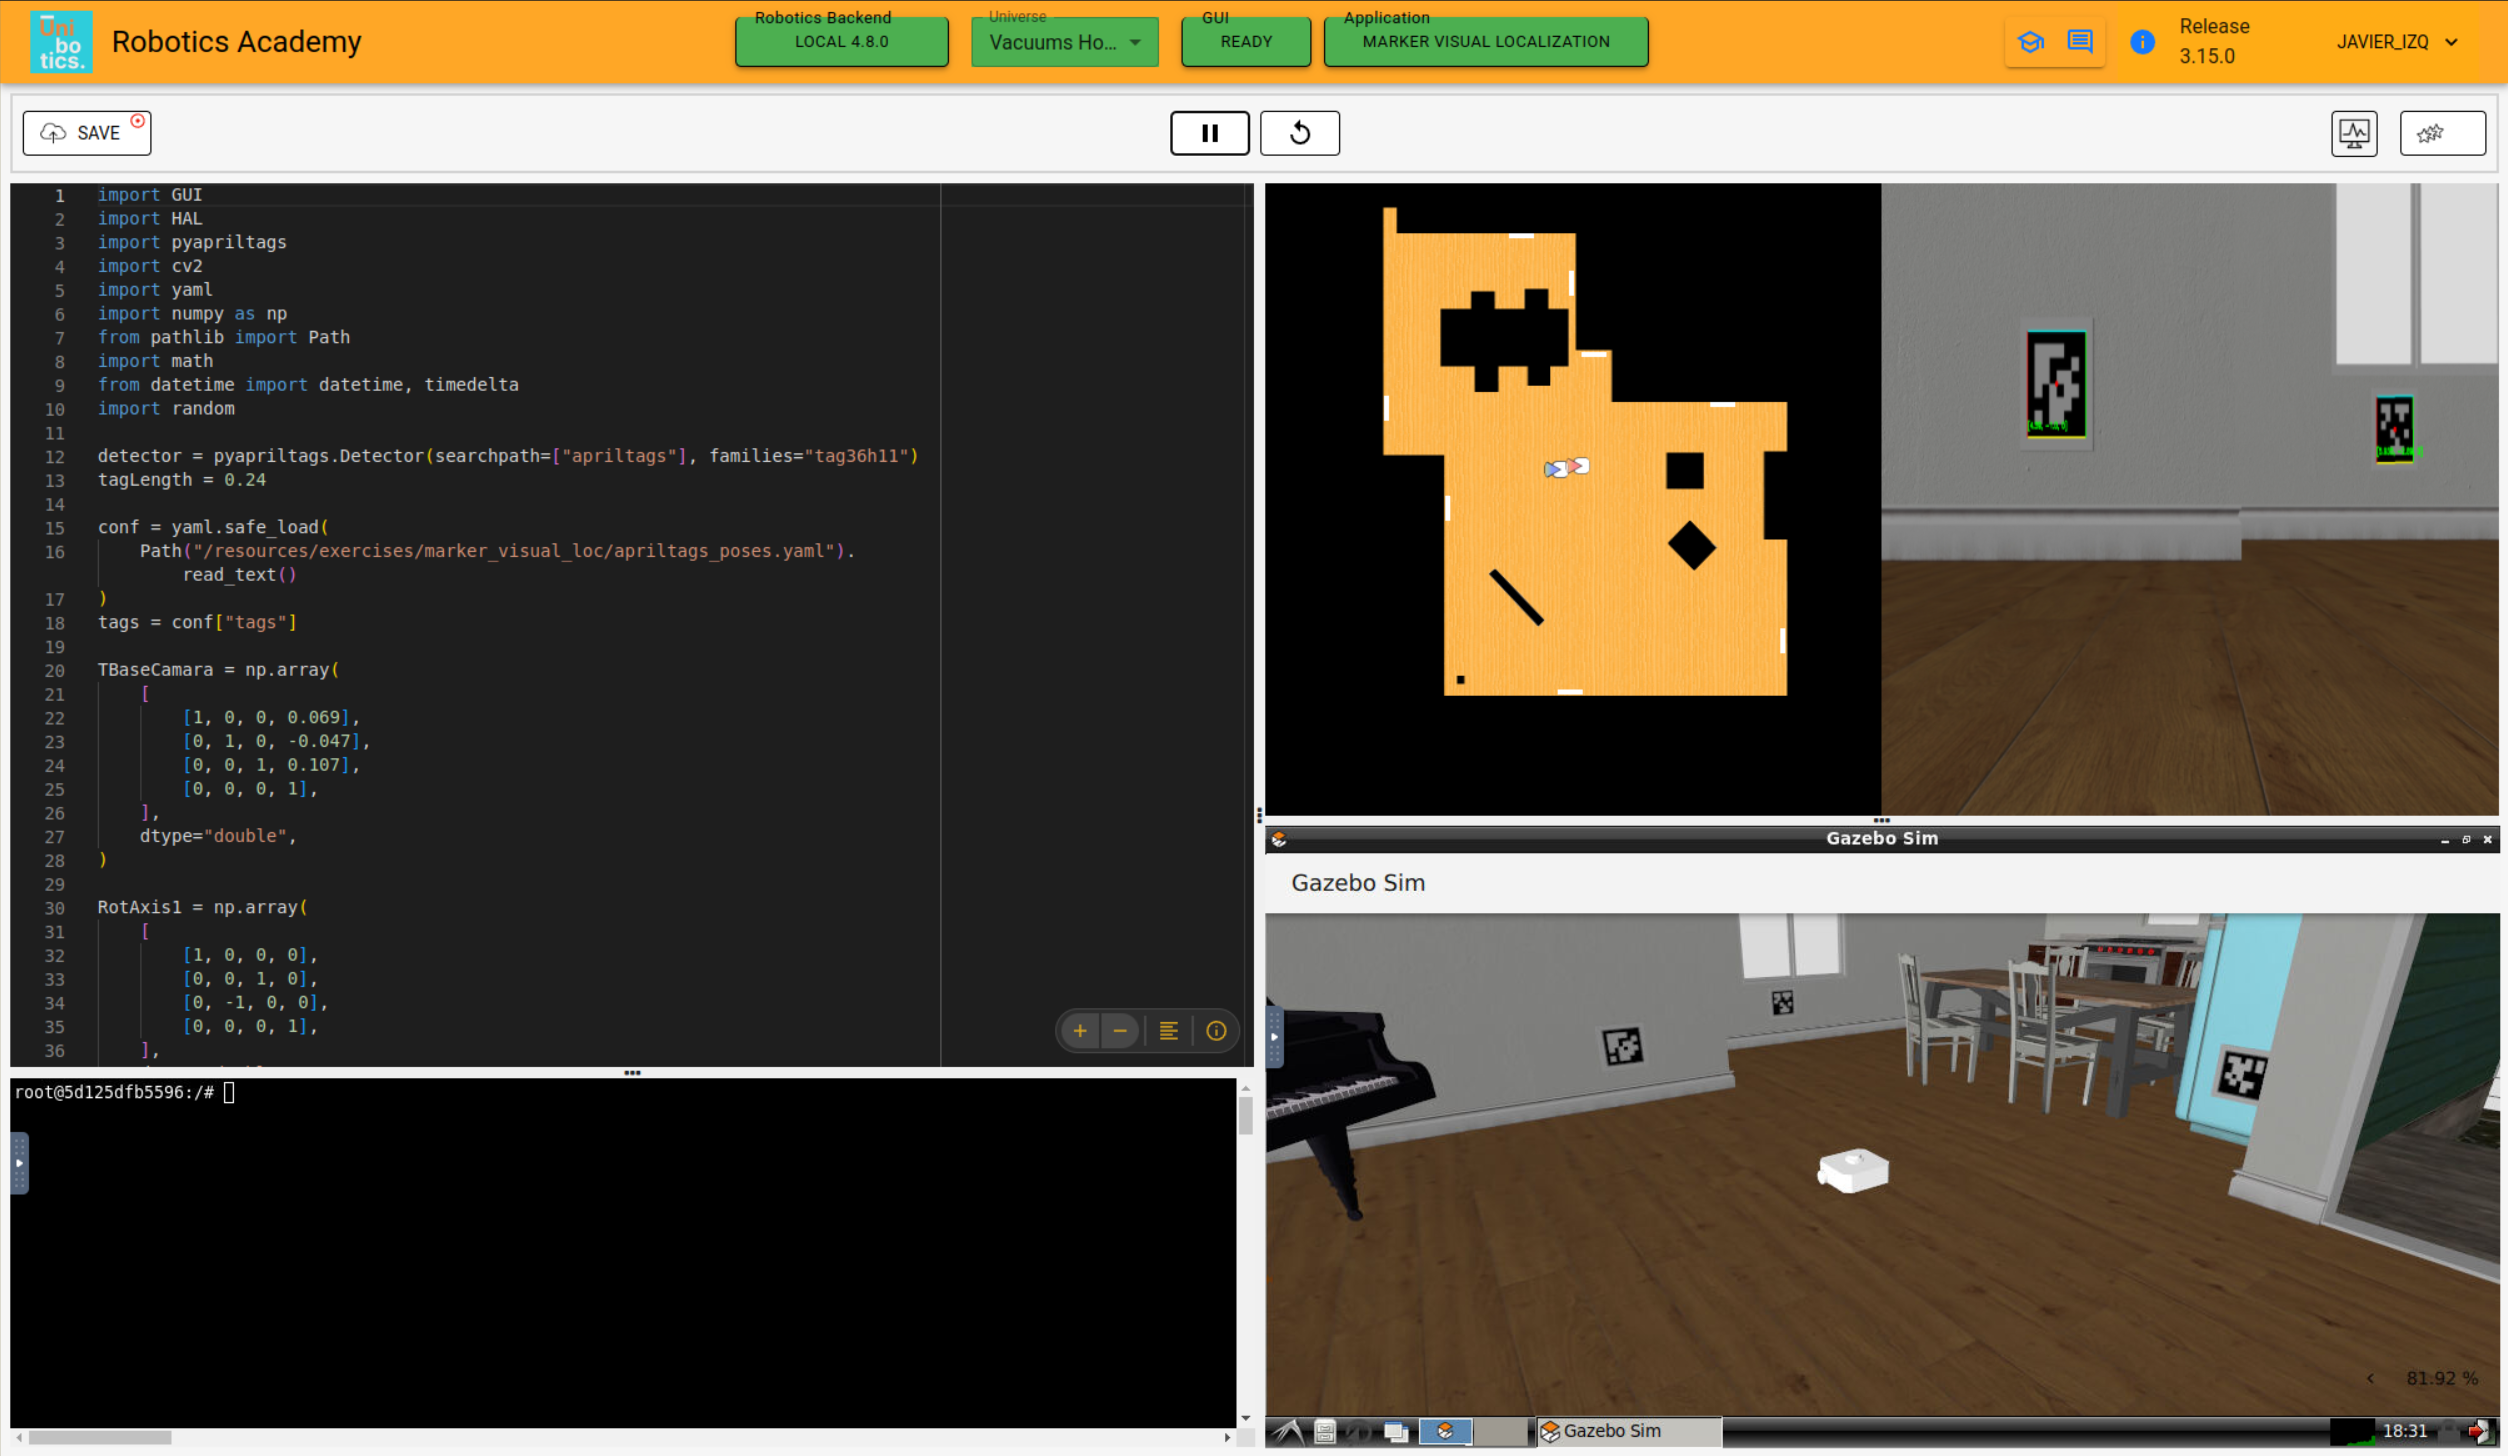
\includegraphics[width=1.0\textwidth]{figures/fundamentos/unib-demo.png}
    \caption{Aplicación robótica básica ejecutando en Unibotics}
    \label{fig:ejemplo}
\end{figure}

Por último, Unibotics, al igual que Robotics Academy, utiliza las bases de datos de universos encontradas en Robotics Infrastructure\footnote{\url{https://github.com/JdeRobot/RoboticsInfrastructure}} que han sido creadas durante este TFG.

Como se ha explicado en los objetivos de este trabajo, la integración en Unibotics es fundamental para el desarrollo y la conclusión de este. 

\subsection{Robotics Backend}\label{sec:robotics-backend}

Robotics Backend\footnote{\url{https://hub.docker.com/r/jderobot/robotics-backend}} es una imagen docker basada en Ubuntu 22.04 que permite lanzar un contenedor con un entorno de desarrollo ROS 2 completo junto con diversas herramientas adicionales. Dentro de este contenedor existe una amplia colección de universos para el simulador Gazebo con sus correspondientes \textit{launchers}.

Para manejar el uso de estas herramientas, se ejecuta dentro de este un programa gestor, llamado \textit{Robotics Application Manager} (RAM). Este es capaz de lanzar universos, preparar las distintas visualizaciones usando visores de VNC y de controlar la ejecución de aplicaciones robóticas. Desde el frontend de la aplicación, ya sea Unibotics, Robotics Academy o BT Studio, que corre en el navegador web, se comunica con el RAM usando websockets para ejecutar las acciones deseadas por estos.

Durante este TFG se ha modificado activamente el contenido del Robotics Backend, ya sea añadiendo soporte para las aplicaciones de BT Studio, los universos personalizados y la funcionalidad extra para el editor de texto en \textit{Robotics Application Manager}, o añadiendo las bases de datos de universos y migrando estos a Gazebo Harmonic en Robotics Infrastructure. 

\subsubsection{Herramientas incluidas en el Robotics Backend}

Las herramientas incluidas dentro del entorno de desarrollo son las siguientes:

\begin{enumerate}
    \item \textbf{ROS2 Humble:}
    \begin{itemize}
        \item Simulador Gazebo Classic.
        \item Simulador Gazebo Harmonic.
        \item RViz2.
    \end{itemize}
    \item \textbf{Python 3.10:}
    \begin{itemize}
        \item websocket\_server.
        \item websockets.
        \item asyncio.
    \end{itemize}
    \item \textbf{Xvfb:} xserver virtual. 
    \item \textbf{Aceleración GPU:} VirtualGL.
    \item \textbf{Servidores VNC:}
    \begin{itemize}
        \item TurboVNC.
        \item noVNC.
    \end{itemize}
    \item \textbf{Dependencias habituales de aplicaciones robóticas:}
    \begin{itemize}
        \item OpenCV.
        \item OMPL.
        \item PyTorch.
        \item TensorFlow.
        \item MoveIt.
        \item AeroStack2.
    \end{itemize}
    \item \textbf{RoboticsInfrastructure}.
    \item \textbf{RoboticsApplicationManager}.
\end{enumerate}

    \chapter{BT Studio: filosofía y estado previo}\label{cap:bt-studio}

En este capítulo se explica el estado de BT Studio al comienzo de este TFG, así como los fundamentos de diseño de la herramienta. Se hará una breve descripción de los componentes antiguos para posteriormente explicar su evolución. Para una explicación más detallada de las bases de BT Studio y su versión antigua se encuentra disponible el TFG que empezó con esta herramienta \cite{TFG_BT_Studio}.

\section{Filosofía}

Como se ha mencionado múltiples veces en capítulos anteriores, el desarrollo de BT Studio sigue una mentalidad \textit{open source} y su código fuente está disponible para toda persona interesada.

Para que la aplicación pueda crecer en el futuro, el diseño de BT Studio está guiado por los siguientes fundamentos básicos, que provienen de las bases de una buena arquitectura software:

\begin{itemize}
    \item \textbf{Claridad:} cada componente del sistema tiene que tener una función concreta y debe tener un nombre claro relacionado con su función.
    \item \textbf{Modularidad:} los componentes deben ser lo más independientes posible entre ellos. De esta forma se permite su reutilización en distintos lugares.
    \item \textbf{Extensibilidad:} facilidad para añadir nuevos componentes al sistema con el mínimo número de cambios en componentes ya existentes. 
\end{itemize}

Además de estos fundamentos, la fiabilidad es indispensable en todo momento, ya que si no lo es, no sería usable BT Studio.

\section{Estado previo}

En esta sección se va a explicar el estado en el que se encontraba BT Studio a la hora de comenzar el TFG, centrándose especialmente en varios aspectos que han sido fundamentales para el desarrollo de las mejoras que se comentarán en el próximo capítulo.

Para explicar de forma resumida esa situación, se puede decir que BT Studio constaba de un frontend básico como el mostrado en la imagen \ref{fig:bt-old-ref}, con un editor visual de árboles de comportamiento y un editor de acciones en Python cuyos ficheros se combinaban usando un traductor para convertir el JSON del BT en un archivo XML junto a las acciones para crear una aplicación robótica. Para más información sobre esto, está disponible el TFG \cite{TFG_BT_Studio}.

\begin{figure}[H]
    \centering
    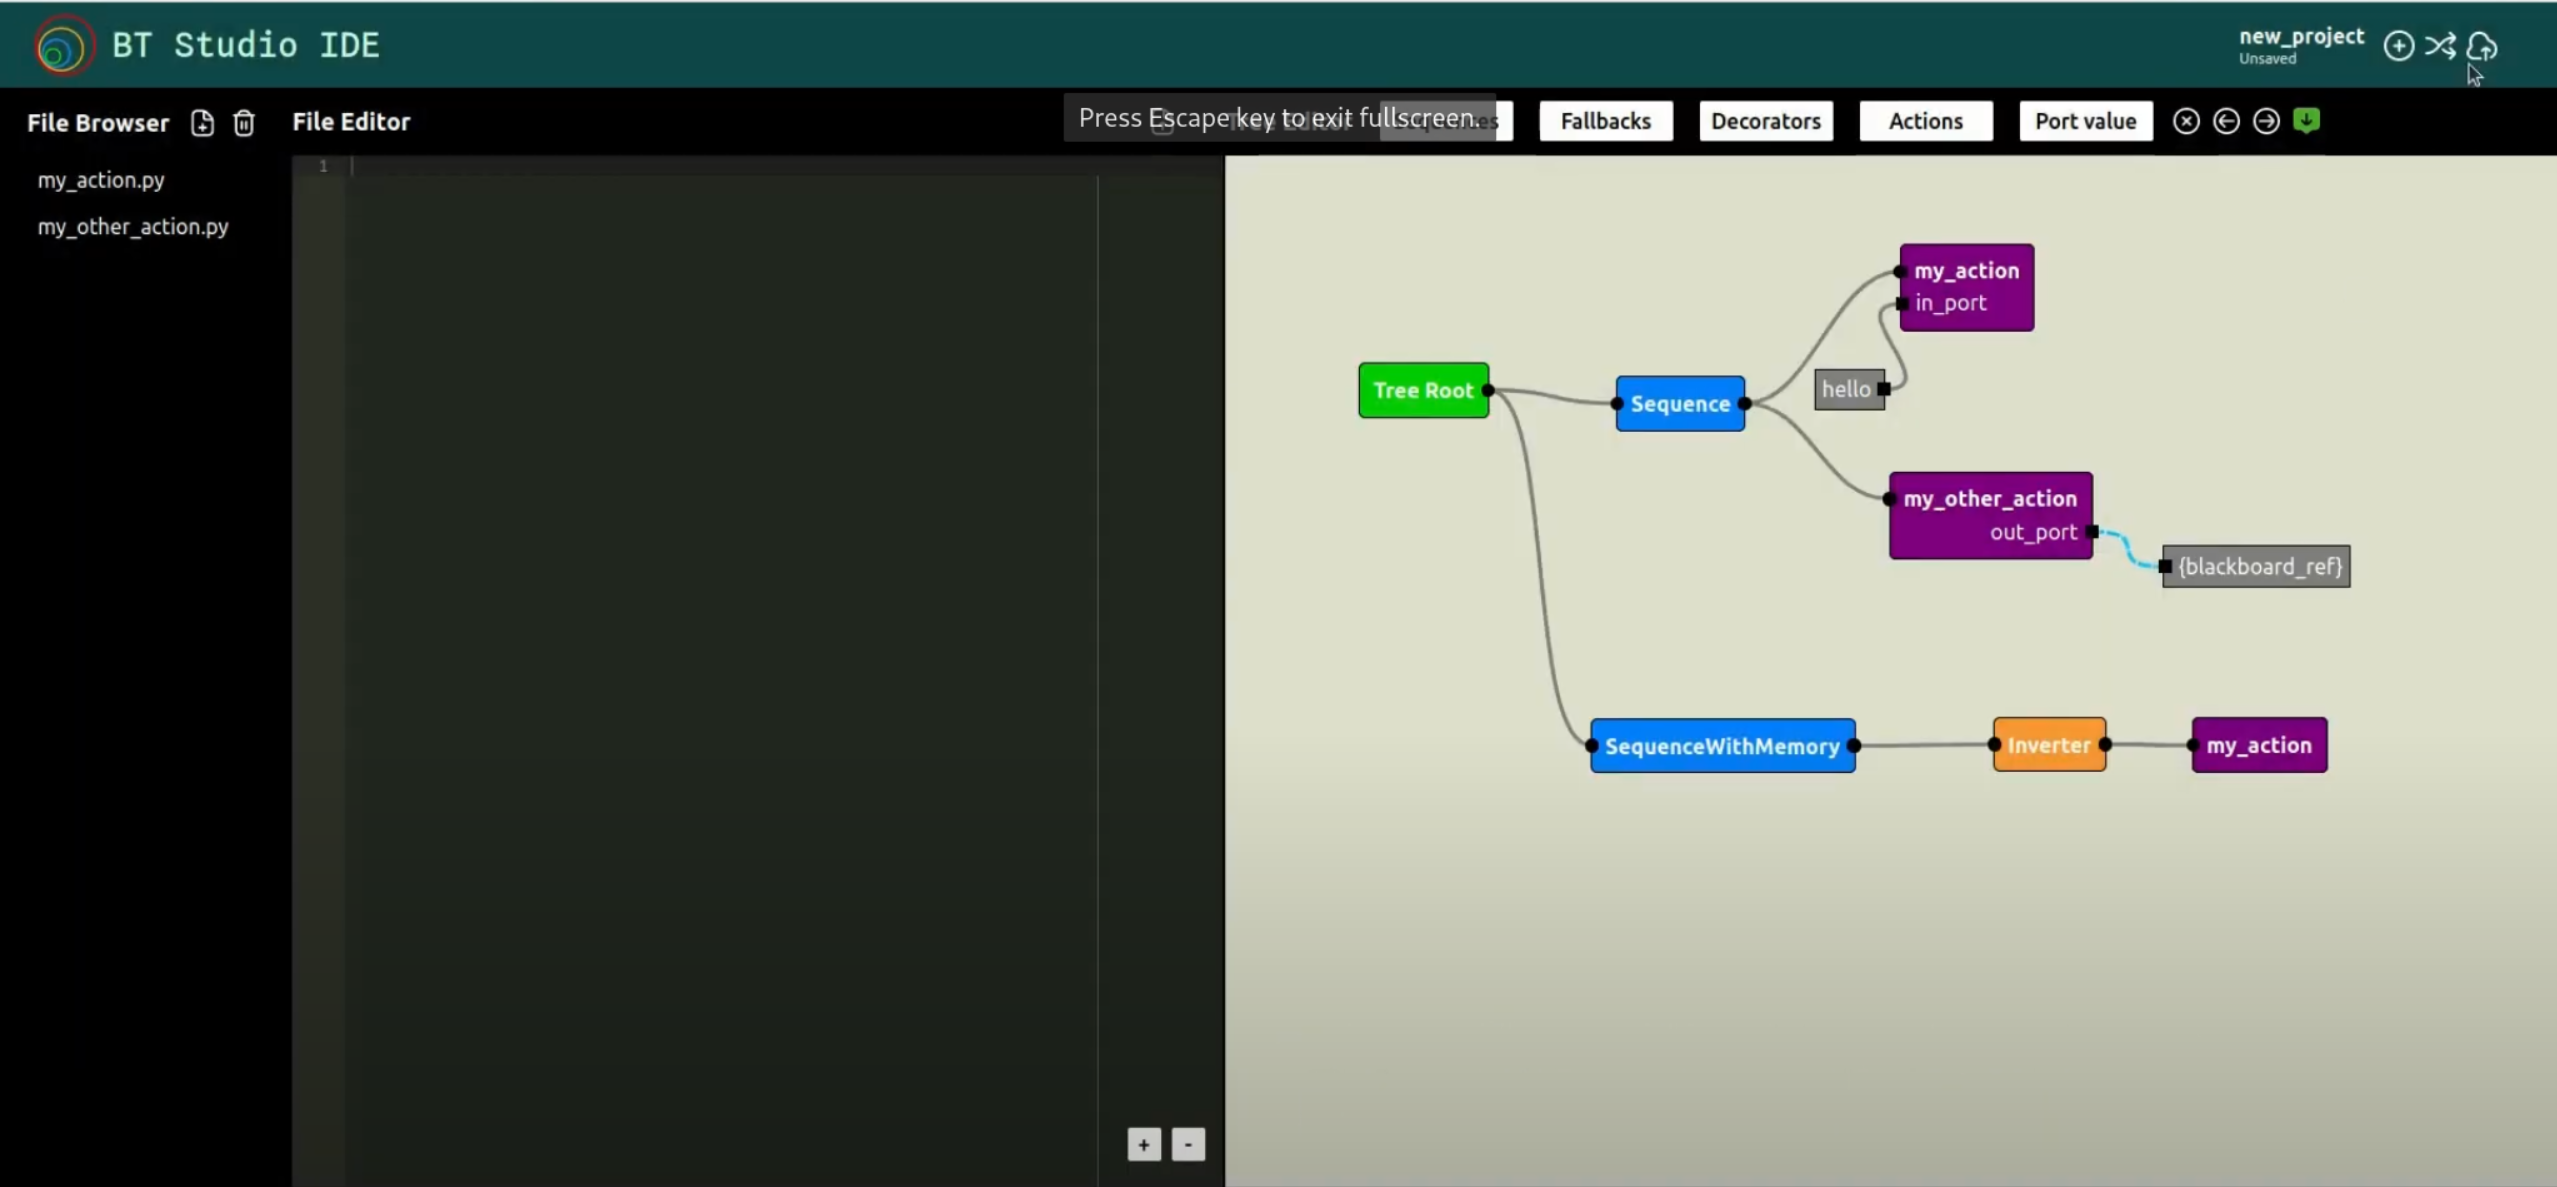
\includegraphics[width=0.8\textwidth]{figures/bt-studio/bt-old.png}
    \caption{Apariencia antigua de BT Studio}
    \label{fig:bt-old-ref}
\end{figure}

Con todo esto, lo que más interesa para las mejoras son los siguientes apartados:

% \subsection{Estructura de la plataforma}

% El objetivo de BT Studio es proporcionar una interfaz web versátil y de fácil uso que permita a los usuarios la creación de aplicaciones robóticas complejas usando árboles de comportamiento. Para esto es necesario establecer las distintas funcionalidades que serán la base de la plataforma:

% \begin{itemize}
%     \item Un IDE web que sirva como interfaz única para el usuario. Desde este, el usuario debe ser capaz de crear diferentes aplicaciones robóticas, guardarlas, editarlas y ejecutarlas. 
%     \item Se debe realizar la traducción desde los ficheros que conforman una aplicación en BT Studio a código ejecutable. Esto debe ocurrir de forma totalmente transparente para el usuario, es decir, que el usuario debe poder ejecutar la aplicación robótica creada en el web IDE sin necesitar configurar nada.
%     \begin{figure}[H]
%         \centering
%         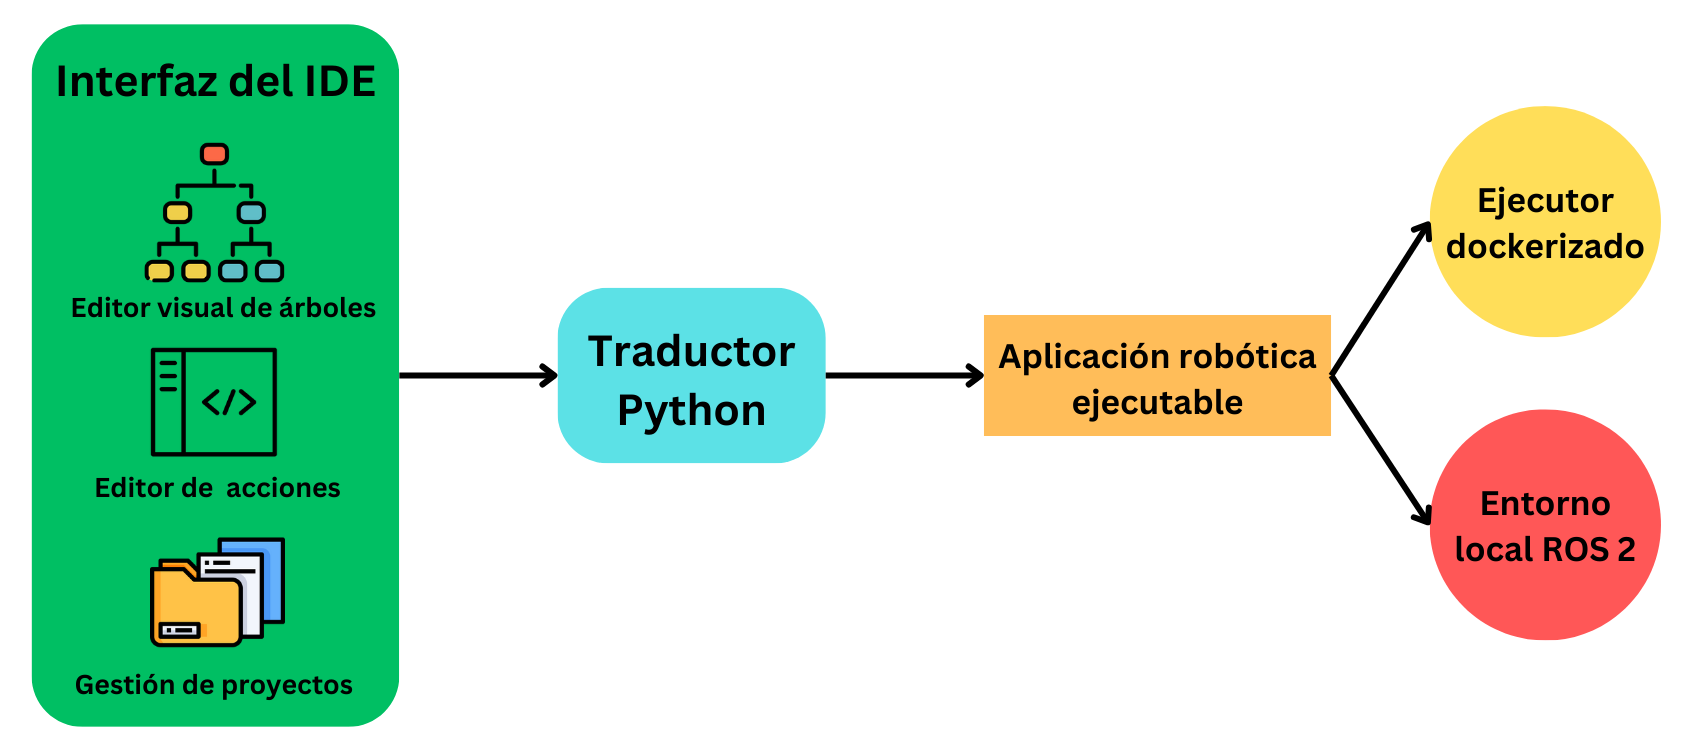
\includegraphics[width=0.9\textwidth]{figures/bt-studio/app_pipeline.png}
%         \caption{Proceso de generación antiguo de aplicaciones en BT Studio}
%         \label{fig:ejemplo}
%     \end{figure}
%     \item Se debe dotar al usuario en el web IDE de herramientas en el web IDE para la visualización y depuración de la ejecución de la aplicación robótica. Esto requiere de al menos proporcionar una interfaz para iniciar, pausar y reiniciar la ejecución que se realice dentro del entorno de ejecución de BT Studio, es decir, en el Robotics Backend, cuyo funcionamiento se explico en el capitulo \ref{cap:tecnologias}.
% \end{itemize}

% Para la comunicación con el RAM (Robotics Application Manager) , el RADI define un protocolo de comunicación a través de WebSockets. BT Studio implementa este protocolo para realizar acciones en el entorno de ejecución desde la interfaz del IDE. 

% \begin{figure}[H]
%     \centering
%     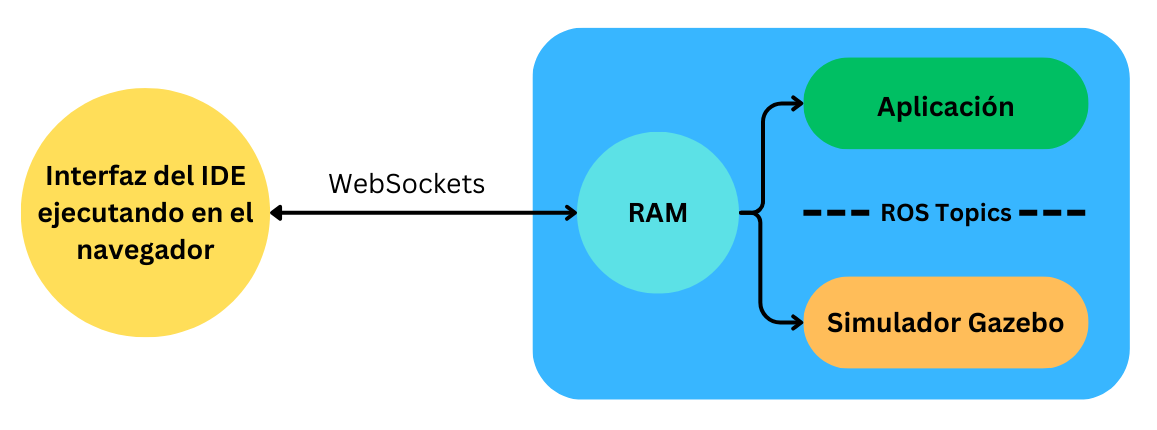
\includegraphics[width=0.9\textwidth]{figures/bt-studio/docker_exec_v2.png}
%     \caption{Ejecución de una aplicación robótica en un entorno dockerizado}
%     \label{fig:ejemplo}
% \end{figure}

\subsection{Definición de aplicaciones robóticas en BT Studio}

En BT Studio, una aplicación robótica basada en árboles de comportamiento está definida por dos componentes: 

\begin{itemize}
    \item \textbf{Acciones:} programada cada una en un fichero Python, siguiendo la estructura estándar para la definición de acciones que proporciona la librería PyTrees. Estas se editan mediante el editor de texto incluido en BT Studio. Cada acción es una clase que implementa distintos métodos propios de un nodo de ejecución de un árbol de comportamiento, como \textit{initialise}, \textit{update} (equivalente a \textit{tick} en PyTrees) o \textit{terminate}. 
    \lstinputlisting[
        float,
        floatplacement=!htp,
        language=Python,
        label=cod:base\_action,
        caption=Estructura de una acción en BT Studio
    ]{code/base_action.py}

    \item \textbf{Árbol de comportamiento:} definidos de manera gráfica mediante el editor visual de BT Studio, que permite definir gráficos personalizados con toda la semántica necesaria para definir un árbol de comportamiento. Estos son guardados en formato JSON. Los nodos de control de flujo disponibles son aquellos definidos por la librería BT.cpp. 
    \begin{figure}[H]
        \centering
        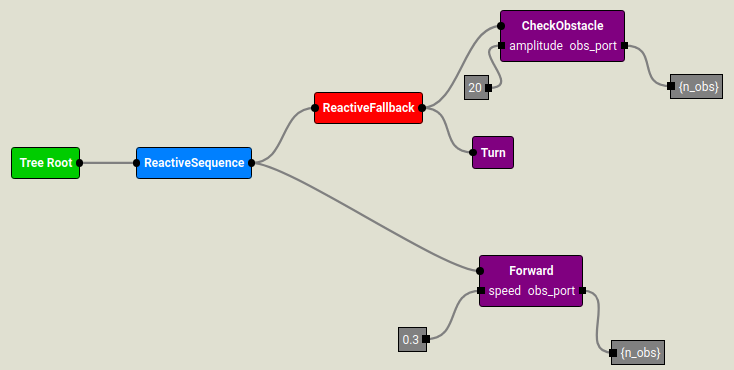
\includegraphics[width=0.7\textwidth]{figures/bt-studio/tree_example.png}
        \caption{Árbol de comportamiento antiguo creado con BT Studio}
        \label{fig:ejemplo}
    \end{figure}
    
\end{itemize}

Todas las aplicaciones que los usuarios crean, editan y ejecutan están basadas en estas funcionalidades básicas. Todos los archivos asociados a una aplicación concreta constituyen un proyecto robótico. 

\subsection{Estructura de un proyecto}\label{sec:bt-struct-old}

La estructura de un proyecto está dividida en dos secciones, el directorio \textit{actions} donde están las acciones y el fichero \textit{graph.json} que guarda el árbol de comportamiento. 

\begin{figure}[H]
    \centering
    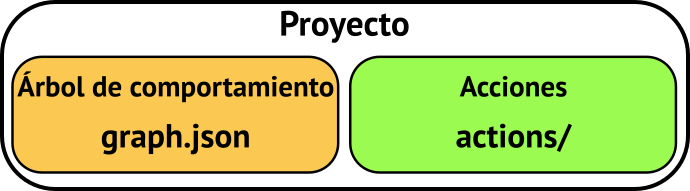
\includegraphics[width=0.7\textwidth]{figures/bt-studio/bt-proy-old.png}
    \caption{Estructura antigua de un proyecto de BT Studio}
    \label{fig:estructura-antigua}
\end{figure}


\subsection{Gestor de comunicaciones: CommsManager}

Este componente se encarga de la comunicación entre el frontend de BT Studio y el entorno de ejecución dockerizada. Implementa distintas funciones para la comunicación mediante mensajes Websocket con un formato determinado. El protocolo concreto para esa comunicación está definido posteriormente en la sección \ref{sec:conex}. 

Este gestor está definido como un \textit{singleton}, es decir, solo se puede crear una instancia, que se pasa a los distintos componentes para que puedan interactuar con el entorno dockerizado. Al ser único, toda la comunicación de este tipo está centralizada para todo BT Studio

\begin{figure}[H]
    \centering
    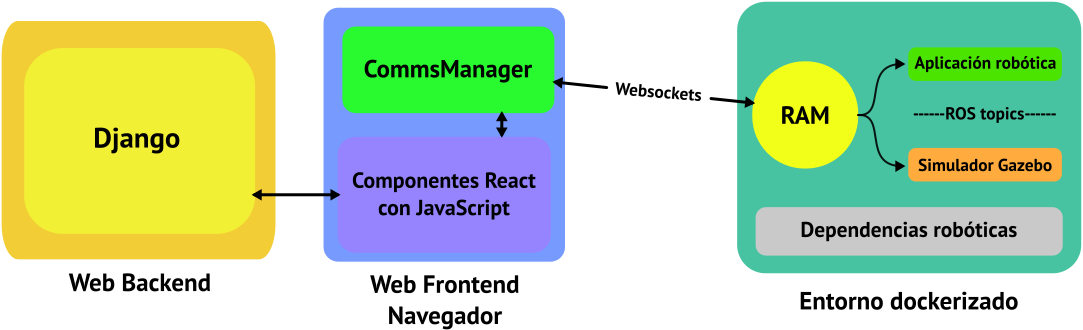
\includegraphics[width=\textwidth]{figures/bt-studio/bt-structure-old.png}
    \caption{Diseño antiguo de la estructura de BT Studio}
    \label{fig:bt-old-old-ref}
\end{figure}
    \chapter{BT Studio: avances}\label{cap:bt-studio-avances}

En este capítulo, se detallarán los avances y contribuciones realizadas en este TFG a la herramienta de BT Studio. Se hablará sobre las mejoras y cambios de sus componentes, así como las implicaciones de estos para la experiencia del usuario.

Todas las siguientes modificaciones han sido realizadas con los fundamentos de BT Studio, definidos en el capítulo \ref{cap:bt-studio}. Estas han mejorado la implementación de esos fundamentos en la herramienta añadiendo funcionalidades adicionales. También se han producido más cambios en la herramienta como parte de un proyecto de GSOC \footnote{\url{https://theroboticsclub.github.io/gsoc2024-Oscar_Martinez/}} centrado en la composición de árboles de comportamiento, externo pero muy relacionado con este TFG.

Todos estos cambios han sido realizados en los siguientes repositorios de GitHub:

\begin{itemize}
    \item \textbf{bt-studio}: \url{https://github.com/JdeRobot/bt-studio}.
    \item \textbf{RoboticsInfrastructure}: \url{https://github.com/JdeRobot/RoboticsInfrastructure}.
    \item \textbf{RoboticsApplicationManager}: \url{https://github.com/JdeRobot/RoboticsApplicationManager}.
    \item \textbf{unibotics-webserver}: es privado.
    \item \textbf{RoboticsBackend}: es privado.
\end{itemize}

\section{Modificaciones al diseño}\label{sec:mod-design}

Para permitir añadir nuevas funcionalidades, ha sido necesario realizar varios cambios en el diseño de la estructura de BT Studio. Estos cambios se van a explicar en más detalle en los siguientes apartados:

\begin{figure}[H]
    \centering
    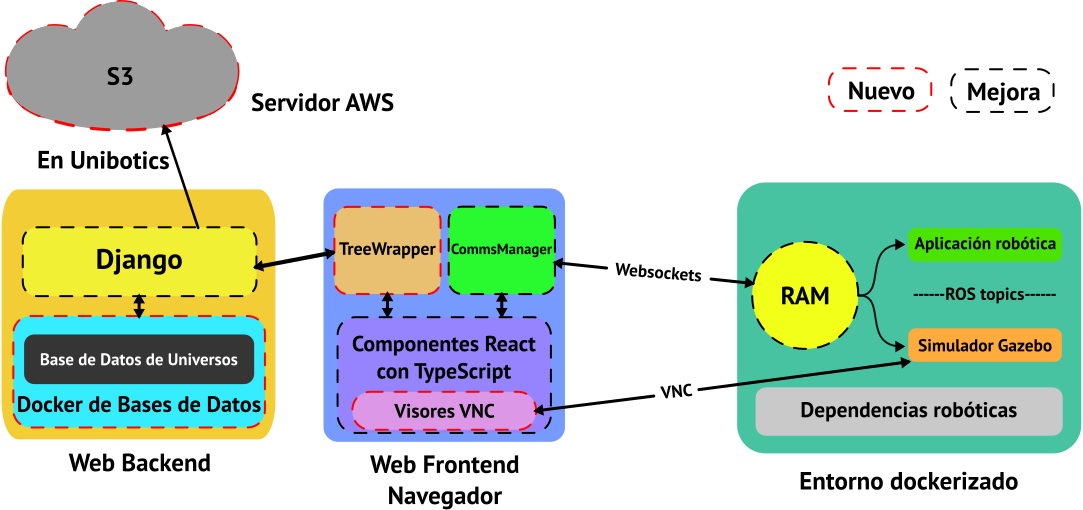
\includegraphics[width=\textwidth]{figures/bt-avances/bt-structure.png}
    \caption{Diseño de la estructura de BT Studio}
    \label{fig:bt-new-struct}
\end{figure}

\subsection{Estructura de un proyecto robótico}

La estructura de un proyecto robótico cualquiera en BT Studio ha sufrido bastantes cambios para poder adaptarse a la inclusión de los universos y permitir una mayor generalización de estos proyectos.

Partiendo de la estructura definida en \ref{sec:bt-struct-old}, se han modificado los siguientes puntos:

\begin{itemize}
    \item División de un proyecto en dos directorios principales: \textit{code} (contiene el código de la aplicación robótica, es decir, sus acciones y su árbol/subárboles) y \textit{universes} (incluye los universos definidos para ese proyecto, que son la combinación de un escenario simulado y un modelo de robot). Además, también se añade el fichero de configuración del proyecto explicado en el apartado a continuación.
    \item Traslado del fichero JSON que guarda el árbol de comportamiento principal al directorio \textit{trees} que se encuentra dentro de \textit{code}. Dentro de este directorio también se alojan los subárboles de comportamiento.
    \item Renombrado el fichero JSON que guarda el árbol de comportamiento principal de \textit{graph.json} a \textit{main.json}.
    \item Incorporación de los universos, que serán explicados con más detalle en la sección \textit{universos}.
\end{itemize}

\begin{figure}[H]
    \centering
    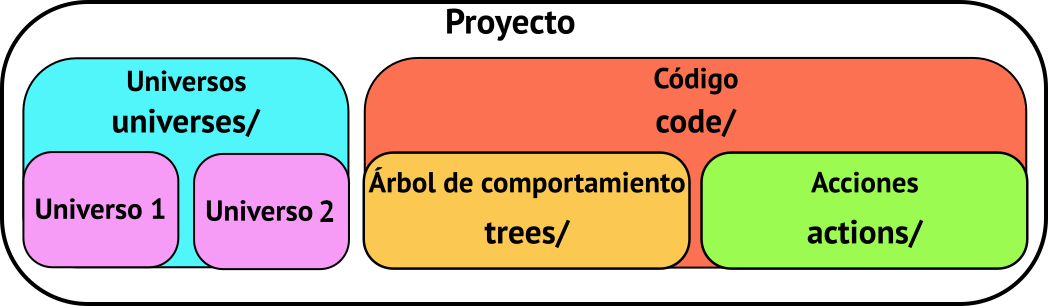
\includegraphics[width=0.7\textwidth]{figures/bt-avances/bt-proy-new.png}
    \caption{Estructura nueva de un proyecto de BT Studio}
    \label{fig:estructura-nueva}
\end{figure}

\subsection{Personalización y configuración}\label{sec:config}

Con el objetivo de permitir al usuario personalizar diferentes aspectos del web IDE, se ha añadido la posibilidad de configurar cada proyecto individualmente. Para conseguir esto, se añadió un fichero JSON extra a la estructura de los proyectos con el fin de guardar la configuración de estos de forma sencilla. Los puntos que pueden ser configurados son los siguientes:

\begin{itemize}
    \item \textbf{theme:} apariencia de BT Studio, permitiendo cambiar entre modo oscuro (\textit{dark}) y claro (\textit{light}).
    \item \textbf{btOrder:} orden de ejecución del árbol de comportamiento. Puede ser de arriba hacia abajo (\textit{top-to-bottom}) o viceversa (\textit{bottom-to-top}).
    \item \textbf{editorShowAccentColors:} mostrar los colores de las acciones en el navegador de ficheros, más detalle en la sección \textit{navegador de ficheros}. Puede ser verdadero (\textit{true}) o falso (\textit{false}).
\end{itemize}

Por otra parte, para permitir al usuario su modificación se han creado un modal en el frontend web y dos funciones en el backend web.

\subsubsection{Frontend}

Empezando por el frontend, primero se debe definir la forma de uso de estas opciones por toda la aplicación. Para esto se ha empleado un elemento de React llamado \textit{context} \footnote{\url{https://react.dev/learn/passing-data-deeply-with-context}}. Este elemento es usado como una alternativa a pasar \textit{props} y que suele ser utilizado cuando un componente React debe pasar información, ya sean funciones o variables, a un gran número de componentes que se encuentran varios niveles más abajo, lo que permite usar estos datos sin tener que pasarlos de forma explícita.

Este \textit{context} se ha usado para crear en el fichero \textit{frontend/src/components/options/Options.tsx} el contexto usando el método de React \textit{createContext} y para crear un componente que va a proveer ese contexto al resto de la aplicación, \textit{OptionsProvider}. Este componente se encarga de encapsular el contexto y las funciones necesarias para modificar las configuraciones que este provee.

Con el proveedor ya creado hace falta añadirlo en la aplicación para que se pueda acceder al contexto. Se añade \textit{OptionsProvider} a BT Studio en el fichero \textit{frontend/src/index.js} para que esté disponible para todos los componentes, que accederán al contexto usando la función \textit{useContext} de React pasándole como parámetro el contexto defindo en \textit{frontend/src/components/options/Options.tsx}.

Ahora que ya está definida la forma de modificar la configuración, nos podemos centrar en la interfaz que usará el usuario para personalizar el proyecto. Para ello se crea el componente \textit{SettingsModal} definido en \textit{frontend/src/components/settings\_popup/SettingsModal.tsx}. En este se muestran las distintas posibles configuraciones en forma de lista, que está dividida en diferentes secciones para indicar el tipo de configuración.

\begin{figure}[H]
    \centering
    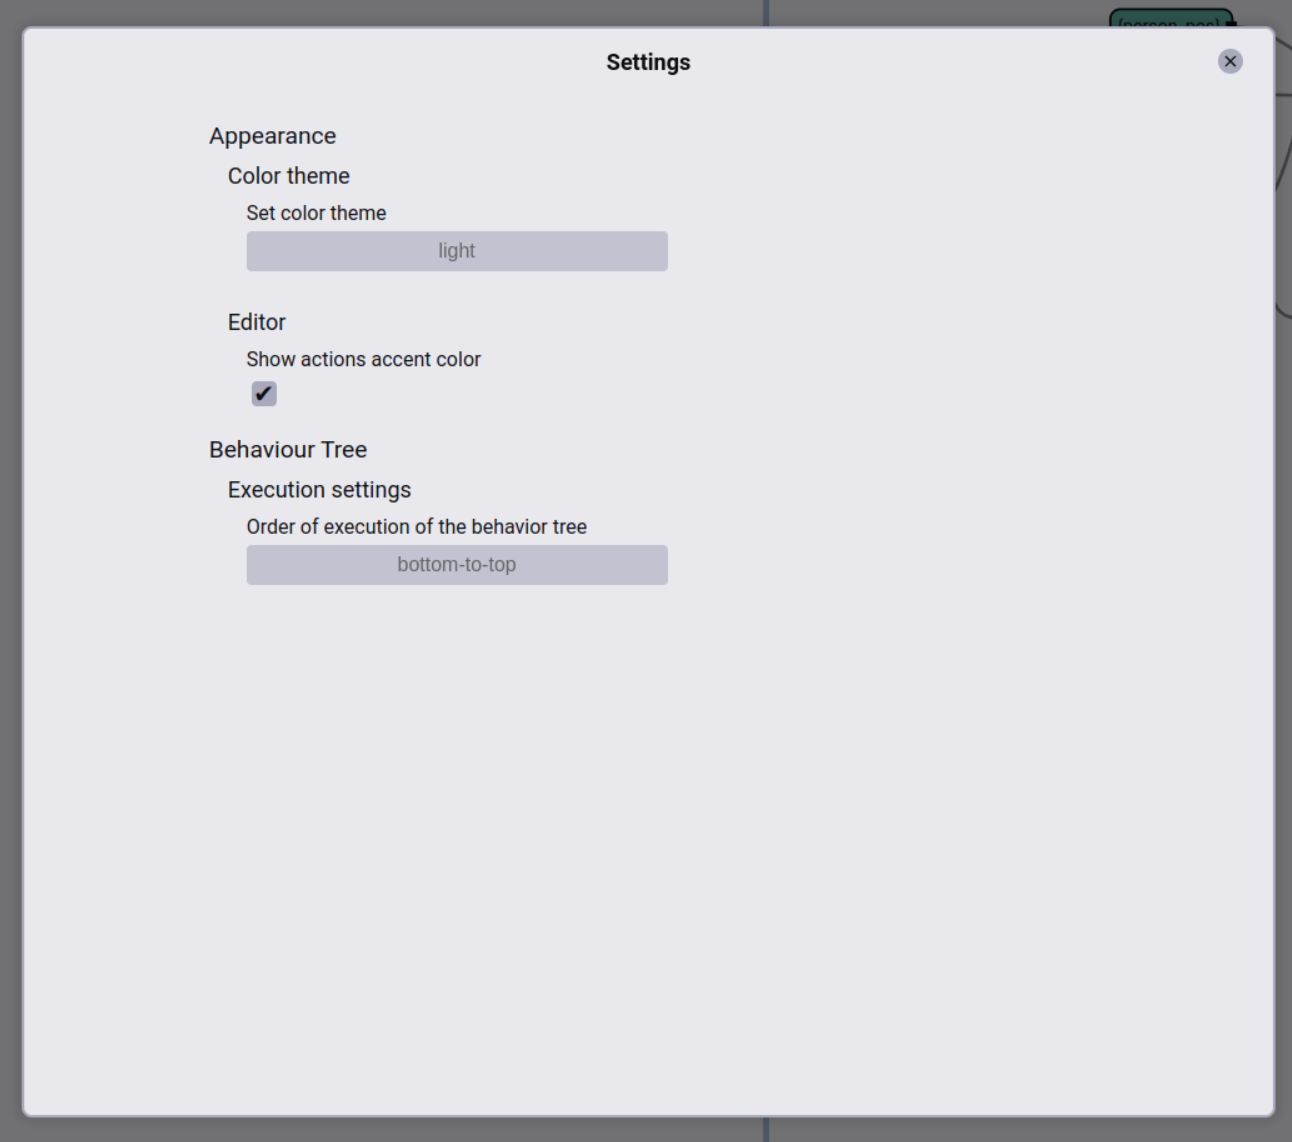
\includegraphics[width=0.5\textwidth]{figures/bt-avances/setting-light.png}
    \caption{Modal de configuración en modo claro de BT Studio}
    \label{fig:ejemplo}
\end{figure}

Cada una de las entradas de los diferentes aspectos de configuración modificar se encuentra estructurada de la misma manera:

\begin{itemize}
    \item Título: muestra dónde se produce el cambio y lo que hace de forma muy resumida.
    \item Descripción: describe de forma más detallada el objetivo de esa configuración.
    \item Configuración: permite editar la configuración. Es una casilla de verificación para aquellas que sus posibles valores son verdadero o falso, y una lista desplegable con los posibles valores para las que tienen múltiples valores definidos previamente.
\end{itemize}

Todas las partes de la estructura anterior están creadas en distintos componentes que se pueden encontrar dentro de los directorios \textit{frontend/src/components/settings\_popup/sections}, para las diferentes secciones, y \textit{frontend/src/components/settings\_popup/options}, para los diferentes tipos de configuraciones. 

\subsubsection{Backend}

Y por último, en la parte del backend se han creado dos funciones nuevas: \textit{save\_project\_configuration} y \textit{get\_project\_configuration}. La primera sirve para guardar los cambios en la configuración y la segunda para devolver el contenido de esta al frontend.

El fichero de configuración está guardado con el formato JSON y con el nombre \textit{config.json}. Un ejemplo de uno de estos ficheros para un proyecto llamado \textbf{MiProyecto} sería:

\lstinputlisting[
    float,
    floatplacement=!htp,
    language=json,
    caption=Ejemplo de un fichero de configuración de un proyecto en BT Studio
]{code/config.json}

\subsection{Estructura de la plataforma}

La estructura de la plataforma ha sufrido unos pequeños cambios en el proceso de generación de aplicaciones, ya que este no era el adecuado de cara a la integración en la plataforma web Unibotics. Esto último se tratará más detalladamente en la sección \ref{sec:bt-unib}.

Los cambios se pueden resumir en la incorporación de un paso intermedio entre la traducción de la aplicación robótica y el ejecutable de la misma. Este paso consiste en el empaquetado de la aplicación y, añadiendo los ficheros necesarios al resultante de la traducción para que se pueda ejecutar en el entorno dockerizado del Robotics Backend o en un entorno local y comprimirlos en forma de archivo ZIP.

\begin{figure}[H]
    \centering
    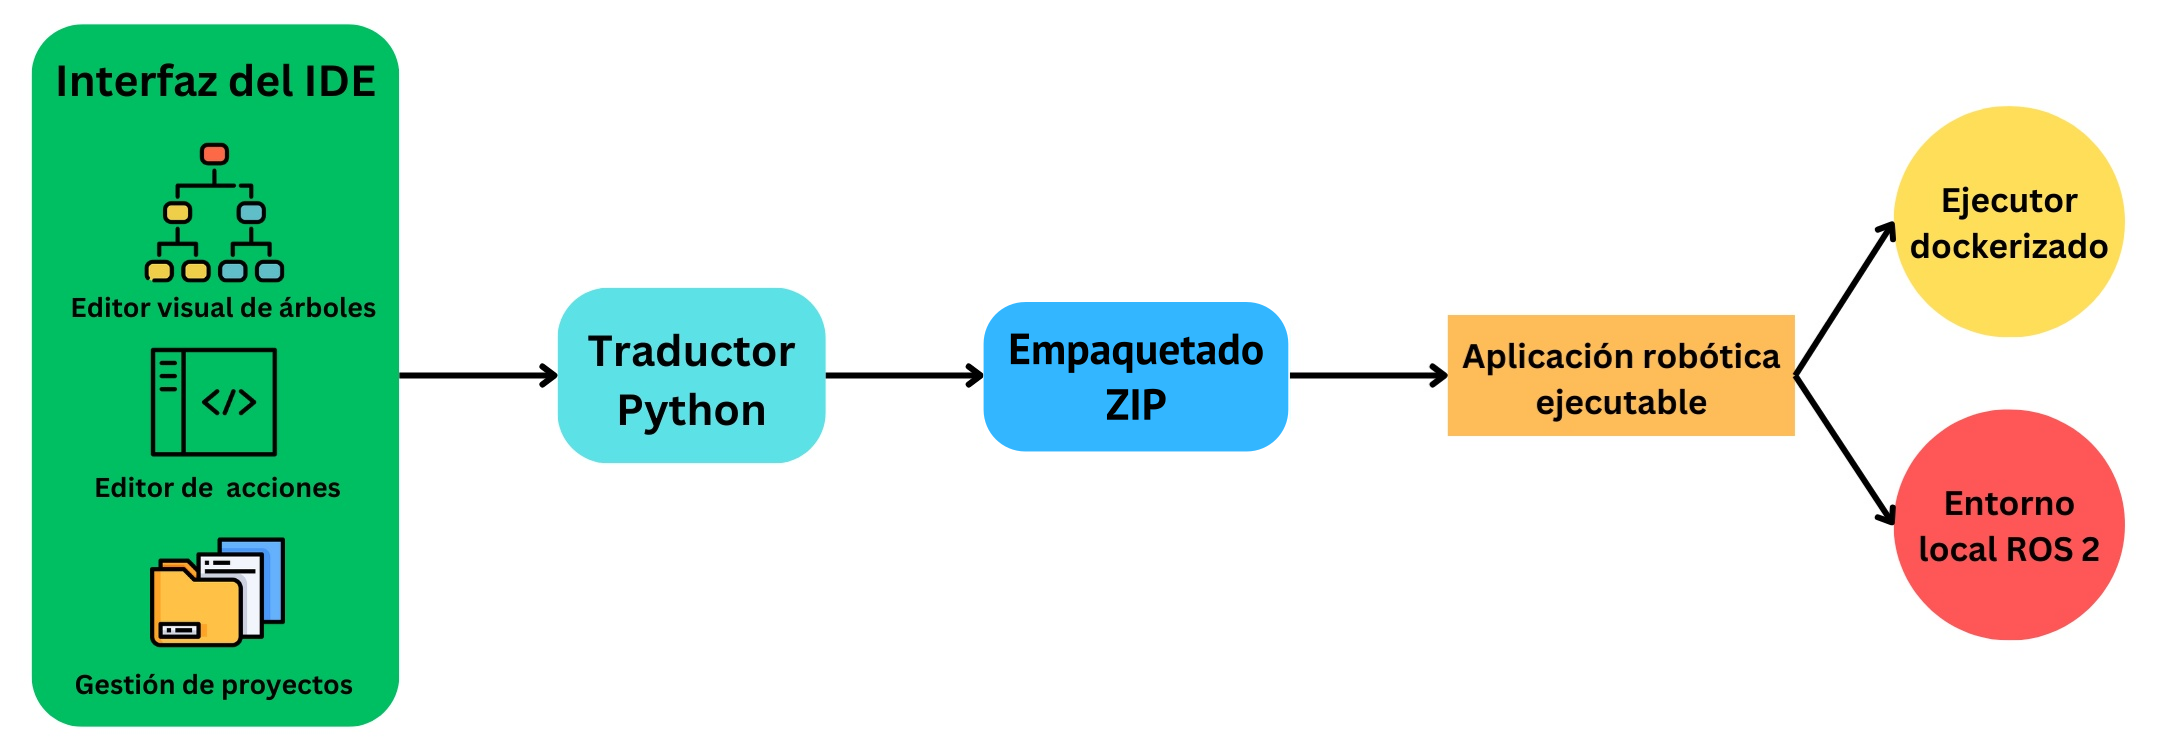
\includegraphics[width=\textwidth]{figures/bt-avances/flow.png}
    \caption{Proceso de generación de aplicaciones en BT Studio}
    \label{fig:ejemplo-23}
\end{figure}

\subsection{Uso exclusivo de TypeScript}

BT Studio estaba compuesto por una mezcla de JavaScript y TypeScript anteriormente. Esto causaba que a veces, por culpa de la naturaleza no tipada de JS, se produjeran errores en ejecución al volverse una variable un tipo no esperado como \textit{null} o \textit{undefined}. Para solucionar todos estos casos se ha migrado todo el código a TS, lo que además ha mejorado la legibilidad y la comprensión del código escrito.

Además, en las partes donde se usaba TS se ha reemplazado todas las definiciones de \textit{any}, que causaban que no se comprobara el tipo, por tipos estrictos.

\subsection{Comunicación con el backend web}

La forma de comunicarse con la API del backend web desde el frontend web ha sido estandarizada y trasladada a un solo fichero de TypeScript llamado \textit{frontend/src/api\_helper/TreeWrapper.ts}.

Anteriormente, esta comunicación usaba tanto el paquete de \textit{axios} \footnote{\url{https://www.npmjs.com/package/axios}} como la función estándar de \textit{fetch} dependiendo del componente, lo que hacía que hubiera múltiples problemas a la hora de modificar una de las funciones del backend dado el distinto funcionamiento de las dos maneras. Para solucionar esto se han sustituido todas las instancias donde se usaba \textit{fetch} por \textit{axios} y se han abstraído todas las llamadas al backend en funciones de TS.

El abstraer y unificar esta comunicación mejora considerablemente el mantenimiento de la aplicación, así como la expansión de la misma.

\subsection{Uso de BT Studio}\label{sec:uso-bt}

Por último, el uso de BT Studio tanto para desarrolladores como usuarios ha cambiado drásticamente. Antes de estas mejoras era necesario la instalación en local del repositorio de BT Studio, así como la de múltiples dependencias como: NPM, Django, yarn, Node.js, múltiples paquetes de Python y múltiples paquetes de JavaScript. Esto, junto con la necesidad de que algunas de estas dependencias necesitaran una versión específica, causaba un gran número de problemas a la hora de instalar y usar BT Studio.

Para solucionarlo, ahora el uso como usuario es enteramente con un contenedor docker (y de forma mixta, Docker y local, para los desarrolladores). Siguiendo el ejemplo de Robotics Academy (se puede considerar la versión offline de Unibotics) se usa una imagen de docker que contiene el Robotics Backend y la aplicación, en este caso BT Studio. Esto permite a los usuarios poder usarlo sin necesidad de descargar el repositorio de BT Studio, ni ninguna dependencia, a excepción de docker, y simplifica su uso a un simple comando.

\lstinputlisting[
    float,
    floatplacement=!htp,
    language=bash,
    label=cod:user\_launch\_BT-Studio,
    caption=Comando para lanzar BT Studio como usuario
]{code/launch-user.txt}

Para los desarrolladores también se simplifica bastante, pero aun así hay una mayor complejidad. Para estos hay que hablar de dos puntos diferentes: el BTDI o BT Studio Docker Image y el script de desarrollador. Para poder acceder a BT Studio usando estos habrá que ir a la dirección \textit{http://0.0.0.0:7164} en el navegador.

\subsubsection{BT Studio Docker Image}

El objetivo de esta imagen docker es permitir al desarrollador crear una imagen de BT Studio igual que las oficiales pero usando las ramas deseadas por este. Esto permite la personalización de la composición del Robotics Backend, es decir, elegir las ramas de Robotics Infrastructure y de Robotics Application Manager.

Todo esto viene empaquetado dentro del script \textit{build.sh} hallado en el directorio \textit{scripts/BTDI}, para una mejor experiencia de uso.

Más información sobre esto en la sección \textit{Ejecución dockerizada} más adelante.

\subsubsection{Script de lanzamiento para desarrolladores}

Para finalizar, ahora que el desarrollador posee la capacidad de crear imágenes docker de BT Studio personalizadas, podemos usar un método similar al usado por los usuarios para lanzar BT Studio. En este caso se utiliza el script llamado \textit{develop.sh} encontrado en el directorio \textit{scripts}.

Este instala las dependencias faltantes, compila el frontend y lanza los contenedores docker usando la herramienta docker-compose explicada en el capítulo \ref{cap:tecnologias}. Esta lanza dos contenedores, uno con las bases de datos correspondientes a los universos, se explicará más detalladamente en la sección \textit{universos}, y otro con la imagen docker oficial de BT Studio o una definida por el desarrollador. La peculiaridad de estos contenedores, es que gracias a docker, se cambia el contenido de las bases de datos de universos y BT Studio por sus contrapartes que se encuentran en local, permitiendo probar las modificaciones a la herramienta de la misma manera que anteriormente.

\section{Backend web del IDE BT Studio}

El backend ha sufrido una ampliación del API para proporcionar no solo una interfaz para la gestión de proyectos, archivos y generación de aplicaciones, sino también para la gestión de universos. En esta sección se explicarán las mejoras realizadas a las funciones ya existentes y las nuevas funciones añadidas para soportar las funcionalidades añadidas en el frontend que estarán explicadas en la próxima sección. 

\subsection{Mejoras}

La funcionalidad básica encargada de la generación de aplicaciones ha sido modificada para permitir que la escalabilidad dentro de la plataforma de Unibotics sea mejor, ya que reduce la cantidad de cómputo en el servidor. Esto se tratará con más detalle en su propia sección, la \textit{integración con Unibotics}, junto con el resto de modificaciones específicas para esa plataforma.

Las modificaciones al resto de funciones serán mostradas en la siguiente lista junto con el nombre de la función en el backend:

\begin{itemize}
    \item \textbf{create\_project:} añadido soporte para la nueva estructura de los proyectos explicada anteriormente.
    \item \textbf{get\_project\_list:} no ha sufrido modificaciones.
    \item \textbf{save\_project\_graph:} renombrado a \textbf{save\_base\_tree} y adaptado a la nueva estructura de los proyectos. 
    \item \textbf{get\_project\_graph:} adaptado a la nueva estructura de los proyectos.
    \item \textbf{get\_file\_list:} cambio en la forma de enumerar los archivos para adecuarse al nuevo navegador de ficheros que se explicará en la siguiente sección. 
    \item \textbf{get\_file:} adaptado a la nueva estructura de los proyectos.
    \item \textbf{create\_file:} adaptado a la nueva estructura de los proyectos y a las nuevas funcionalidades del nuevo navegador de ficheros.
    \item \textbf{delete\_file:} adaptado a la nueva estructura de los proyectos.
    \item \textbf{save\_file:} adaptado a la nueva estructura de los proyectos.
    \item \textbf{generate\_app:} renombrado a \textbf{generate\_local\_app}. Reimplementación completa para adecuarlo a su uso en Unibotics, esto será explicado con más detalle en un apartado de la sección \textit{ejecución dockerizada}.
    \item \textbf{get\_dockerized\_app:} reimplementación completa para adecuarlo a su uso en Unibotics, esto será explicado con más detalle en la sección \textit{ejecución dockerizada}.
\end{itemize}

\subsection{Novedades}

Al igual que se han modificado la mayoría de las funciones antiguas para adaptarse a las novedades del frontend, también se han añadido nuevas funciones. Estas adiciones están estrechamente relacionadas con sus contrapartes en el frontend y la mayoría se explicarán en más detalle en sus respectivas secciones o apartados más adelante.

La lista de las funciones añadidas al backend es la siguiente:

\begin{itemize}
    \item \textbf{save\_project\_configuration:} guarda la configuración del proyecto actualizada.
    \item \textbf{get\_project\_configuration:} devuelve la configuración del proyecto.
    \item \textbf{delete\_project:} permite eliminar un proyecto existente, borrando todos los ficheros incluidos dentro de este.
    \item \textbf{upload\_universe:} permite subir un universo propio del usuario en forma de fichero ZIP, además genera los directorios y la configuración necesaria.
    \item \textbf{add\_docker\_universe:} crea un nuevo universo usando los disponibles en el Robotics Backend, además genera los directorios y la configuración necesaria.
    \item \textbf{delete\_universe:} elimina un universo existente, borrando todos los ficheros incluidos dentro de este.
    \item \textbf{get\_universes\_list:} enumera todos los universos existentes.
    \item \textbf{get\_universe\_zip:} genera un archivo ZIP con todos los ficheros necesarios para el lanzamiento del universo en el Robotics Backend. Esto solo está disponible para los universos que no son del Robotics Backend.
    \item \textbf{get\_universe\_configuration:} devuelve la configuración del universo correspondiente.
    \item \textbf{list\_docker\_universes:} devuelve una lista de todos los universos disponibles en el Robotics Backend, permitiendo al usuario seleccionar el universo deseado. Usa la base de datos de universos para mostrar esta información.
    \item \textbf{get\_docker\_universe\_path:} devuelve información adicional sobre el universo, si este está disponible en el Robotics Backend. Usa la base de datos de universos para mostrar esta información.
    \item \textbf{get\_tree\_structure:} devuelve la estructura básica del árbol de comportamiento que será usada en el monitor de ejecución.
    \item \textbf{get\_subtree\_structure:} devuelve la estructura básica del subárbol de comportamiento que será usada en el monitor de ejecución.
    \item \textbf{rename\_file:} permite renombrar un archivo.
    \item \textbf{create\_folder:} crea un nuevo directorio vacío en la ubicación especificada en el nuevo navegador de ficheros.
    \item \textbf{rename\_folder:} permite renombrar un directorio.
    \item \textbf{delete\_folder:} elimina un directorio específico y todos sus contenidos.
    \item \textbf{upload\_code:} permite subir múltiples ficheros comprimidos en un solo archivo ZIP en la ubicación especificada en el nuevo navegador de ficheros.
    \item \textbf{create\_action:} permite crear el archivo necesario para una nueva acción a partir de diferentes plantillas, que son especificadas en el nuevo modal de creación de acciones.
    \item \textbf{get\_actions\_list:} enumera todas las acciones existentes.
\end{itemize}

\subsection{Mejoras en el traductor}

Por último, también se ha introducido una mejora en el traductor de JSON a XML. Para poder aplicar de manera correcta las dos variantes en el orden de ejecución del árbol de comportamiento introducido en el apartado \ref{sec:config} ha hecho falta añadir al traductor la capacidad de ordenar los nodos por la altura a la que se encuentran en el diagrama. Esto permite que varios nodos pertenecientes a la misma profundidad del árbol se ordenen de forma correcta para su traducción a XML.

\section{Frontend web del IDE BT Studio}\label{sec:bt-frontend}

En esta sección se va a hablar sobre las mejoras realizadas en el frontend de BT Studio. Estas no tienen que afectar exclusivamente a la experiencia del usuario, sino que también se centran en la mejora de la organización del frontend.

A todos los cambios que se van a presentar a continuación hay que sumarle aquellos presentados en la sección \ref{sec:mod-design}, como la creación de configuraciones, el uso de TypeScript o la mejora de la comunicación con el backend web. A estos se añaden los que van a ser explicados en sus secciones particulares, como el navegador de archivos, el modal de universos o el monitor de ejecución.

Dicho esto, las mejoras y adiciones que se van a presentar a continuación mezclarán los modos gráficos claros y oscuros de manera aleatoria donde haya imágenes disponibles.

También se ha modificado el icono de la asociación de JdeRobot por el icono de Unibotics solo en la versión \textit{online}, que además devuelve al usuario a la página de inicio de Unibotics.

\begin{figure}[H]
    \centering
    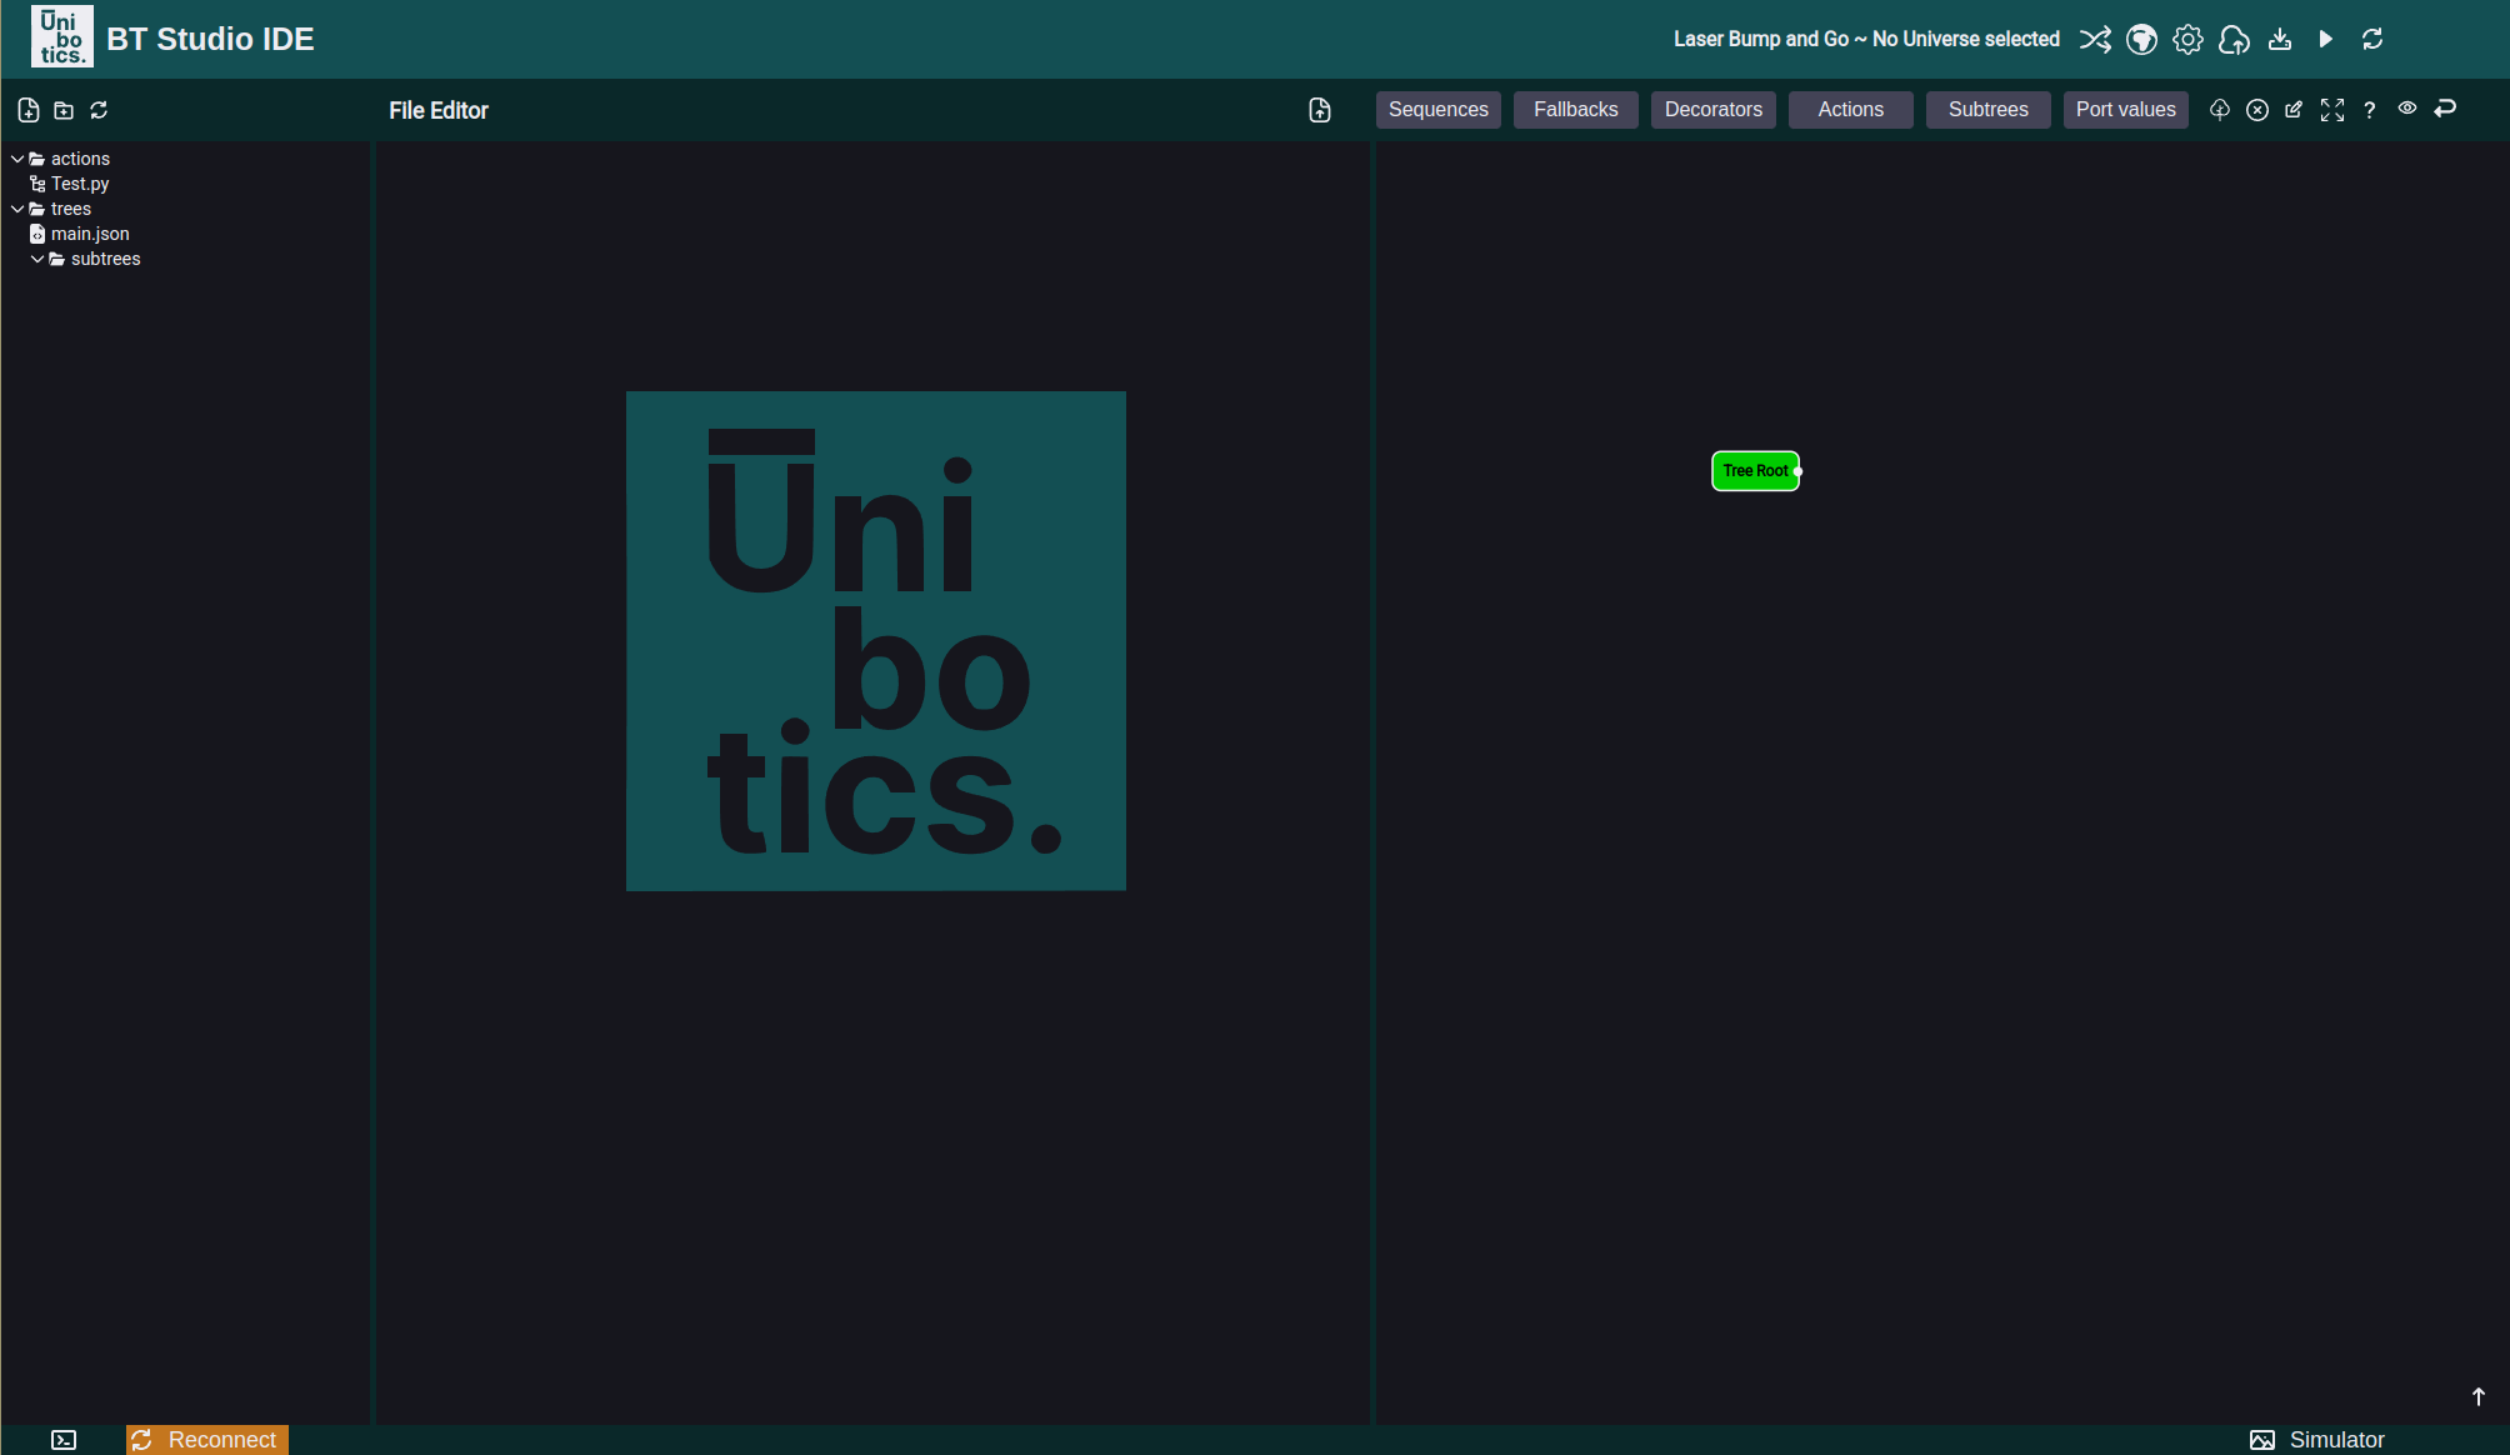
\includegraphics[width=0.9\textwidth]{figures/bt-avances/bt-unib.png}
    \caption{Apariencia de un proyecto nuevo de BT Studio en Unibotics}
    \label{fig:bt-unib}
\end{figure}

\subsection{Listado de componentes de React}

Esta sección no es una mejora, pero sirve de introducción para las que se introducirán posteriormente. Los componentes de React principales de BT Studio son:

\begin{itemize}
    \item \textbf{ErrorModal}: contiene el modal para los \textit{popups}.
    \item \textbf{FileBrowser}: contiene todo el navegador de ficheros.
    \item \textbf{FileEditor}: contiene todo el editor de ficheros Monaco.
    \item \textbf{HeaderMenu}: contiene la cabecera de BT Studio y los siguientes componentes:
    \begin{itemize}
        \item \textbf{UniverseModal}: contiene el modal para lo gestión y creación de universos.
        \item \textbf{ProjectModal}: contiene el modal para lo gestión y creación de proyectos.
    \end{itemize}
    \item \textbf{SettingsModal}: contiene el modal para las configuraciones.
    \item \textbf{StatusBar}: contiene la barra de estado.
    \item \textbf{MainTreeEditorContainer}: contiene los siguientes componentes:
    \begin{itemize}
        \item \textbf{DiagramEditor}: contiene el editor de árboles de comportamiento.
        \item \textbf{NodeMenu}: contiene los modales y acciones para el editor de árboles de comportamiento.
        \item \textbf{DiagramVisualizer}: contiene el monitor de árboles de comportamiento.
    \end{itemize}
    \item \textbf{VncViewer}: contiene el visor VNC del simulador.
    \item \textbf{TerminalViewer}: contiene el visor VNC del simulador.
\end{itemize}

\subsection{Mejora del CSS}

Esta mejora no se refleja directamente para el usuario, pero ha sido fundamental a la hora de implementar una interfaz coherente y permitir el uso de múltiples aspectos, modo claro y oscuro. La mejora ha tenido como objetivos los siguientes:

\begin{itemize}
    \item Uso de variables en el CSS para controlar los colores de los componentes.
    \item Definición de esas variables en un solo fichero, junto con los temas.
    \item Estandarización del tamaño de \textit{padding} y bordes de los componentes.
    \item Reimplementación de componentes definidos usando valores absolutos como \textit{Flexbox}.
\end{itemize}

Los dos primeros puntos han estado basados en la introducción de las variables de CSS en el código existente. Estas han sido usadas porque tienen un ámbito global y permiten que al cambiar su contenido, todas las instancias que la usan son actualizadas con este. El siguiente \textit{snippet} de código \ref{cod:css} pertenece a una versión simplificada de su uso en BT Studio.

Por último, los componentes React que usaban valores absolutos para su correcta colocación han sido reemplazados con componentes que usan el diseño \textit{Flexbox}, que permite alinear los componentes hijos en diferentes puntos usando las propiedades \textit{flex-direction}, \textit{flex-wrap}, \textit{flex-flow}, \textit{justify-content}, \textit{align-items}, \textit{align-content}. Esto consigue que los componentes se muestren de forma correcta en diferentes tamaños de pantalla.

\lstinputlisting[
    float,
    floatplacement=!htp,
    language=css,
    label=cod:css,
    caption=Ejemplo del uso de variables de CSS en BT Studio
]{code/App.css}

\subsection{Mejora de la interfaz}

La interfaz del web IDE ha tenido que ser actualizada para estar más a la última en temas de diseño y para encajar los nuevos componentes como los visores para la ejecución dockerizada que se explicarán más adelante en su propia sección.

La nueva interfaz gráfica consta de las siguientes partes que se muestran en la Figura \ref{fig:bt-int}:

\begin{itemize}
    \item Encabezado: tiene los botones para mostrar los modales de proyectos, universos y configuración, el guardado, la descarga del proyecto y el control de la ejecución. 
    \item Navegador de ficheros: permite abrir, crear y borrar ficheros y directorios. Con más detalle en su propia sección.
    \item Editor de ficheros: permite editar los ficheros y acciones del proyecto. Con más detalle en su propia sección.
    \item Barra de estado: permite controlar y ver el estado de la conexión con el entorno de ejecución dockerizada. Con más detalle en su propia sección.
    \item Editor de árboles de comportamiento: permite editar de manera visual los árboles de comportamiento. Con más detalle en su propia sección.
\end{itemize}

\begin{figure}[H]
    \centering
    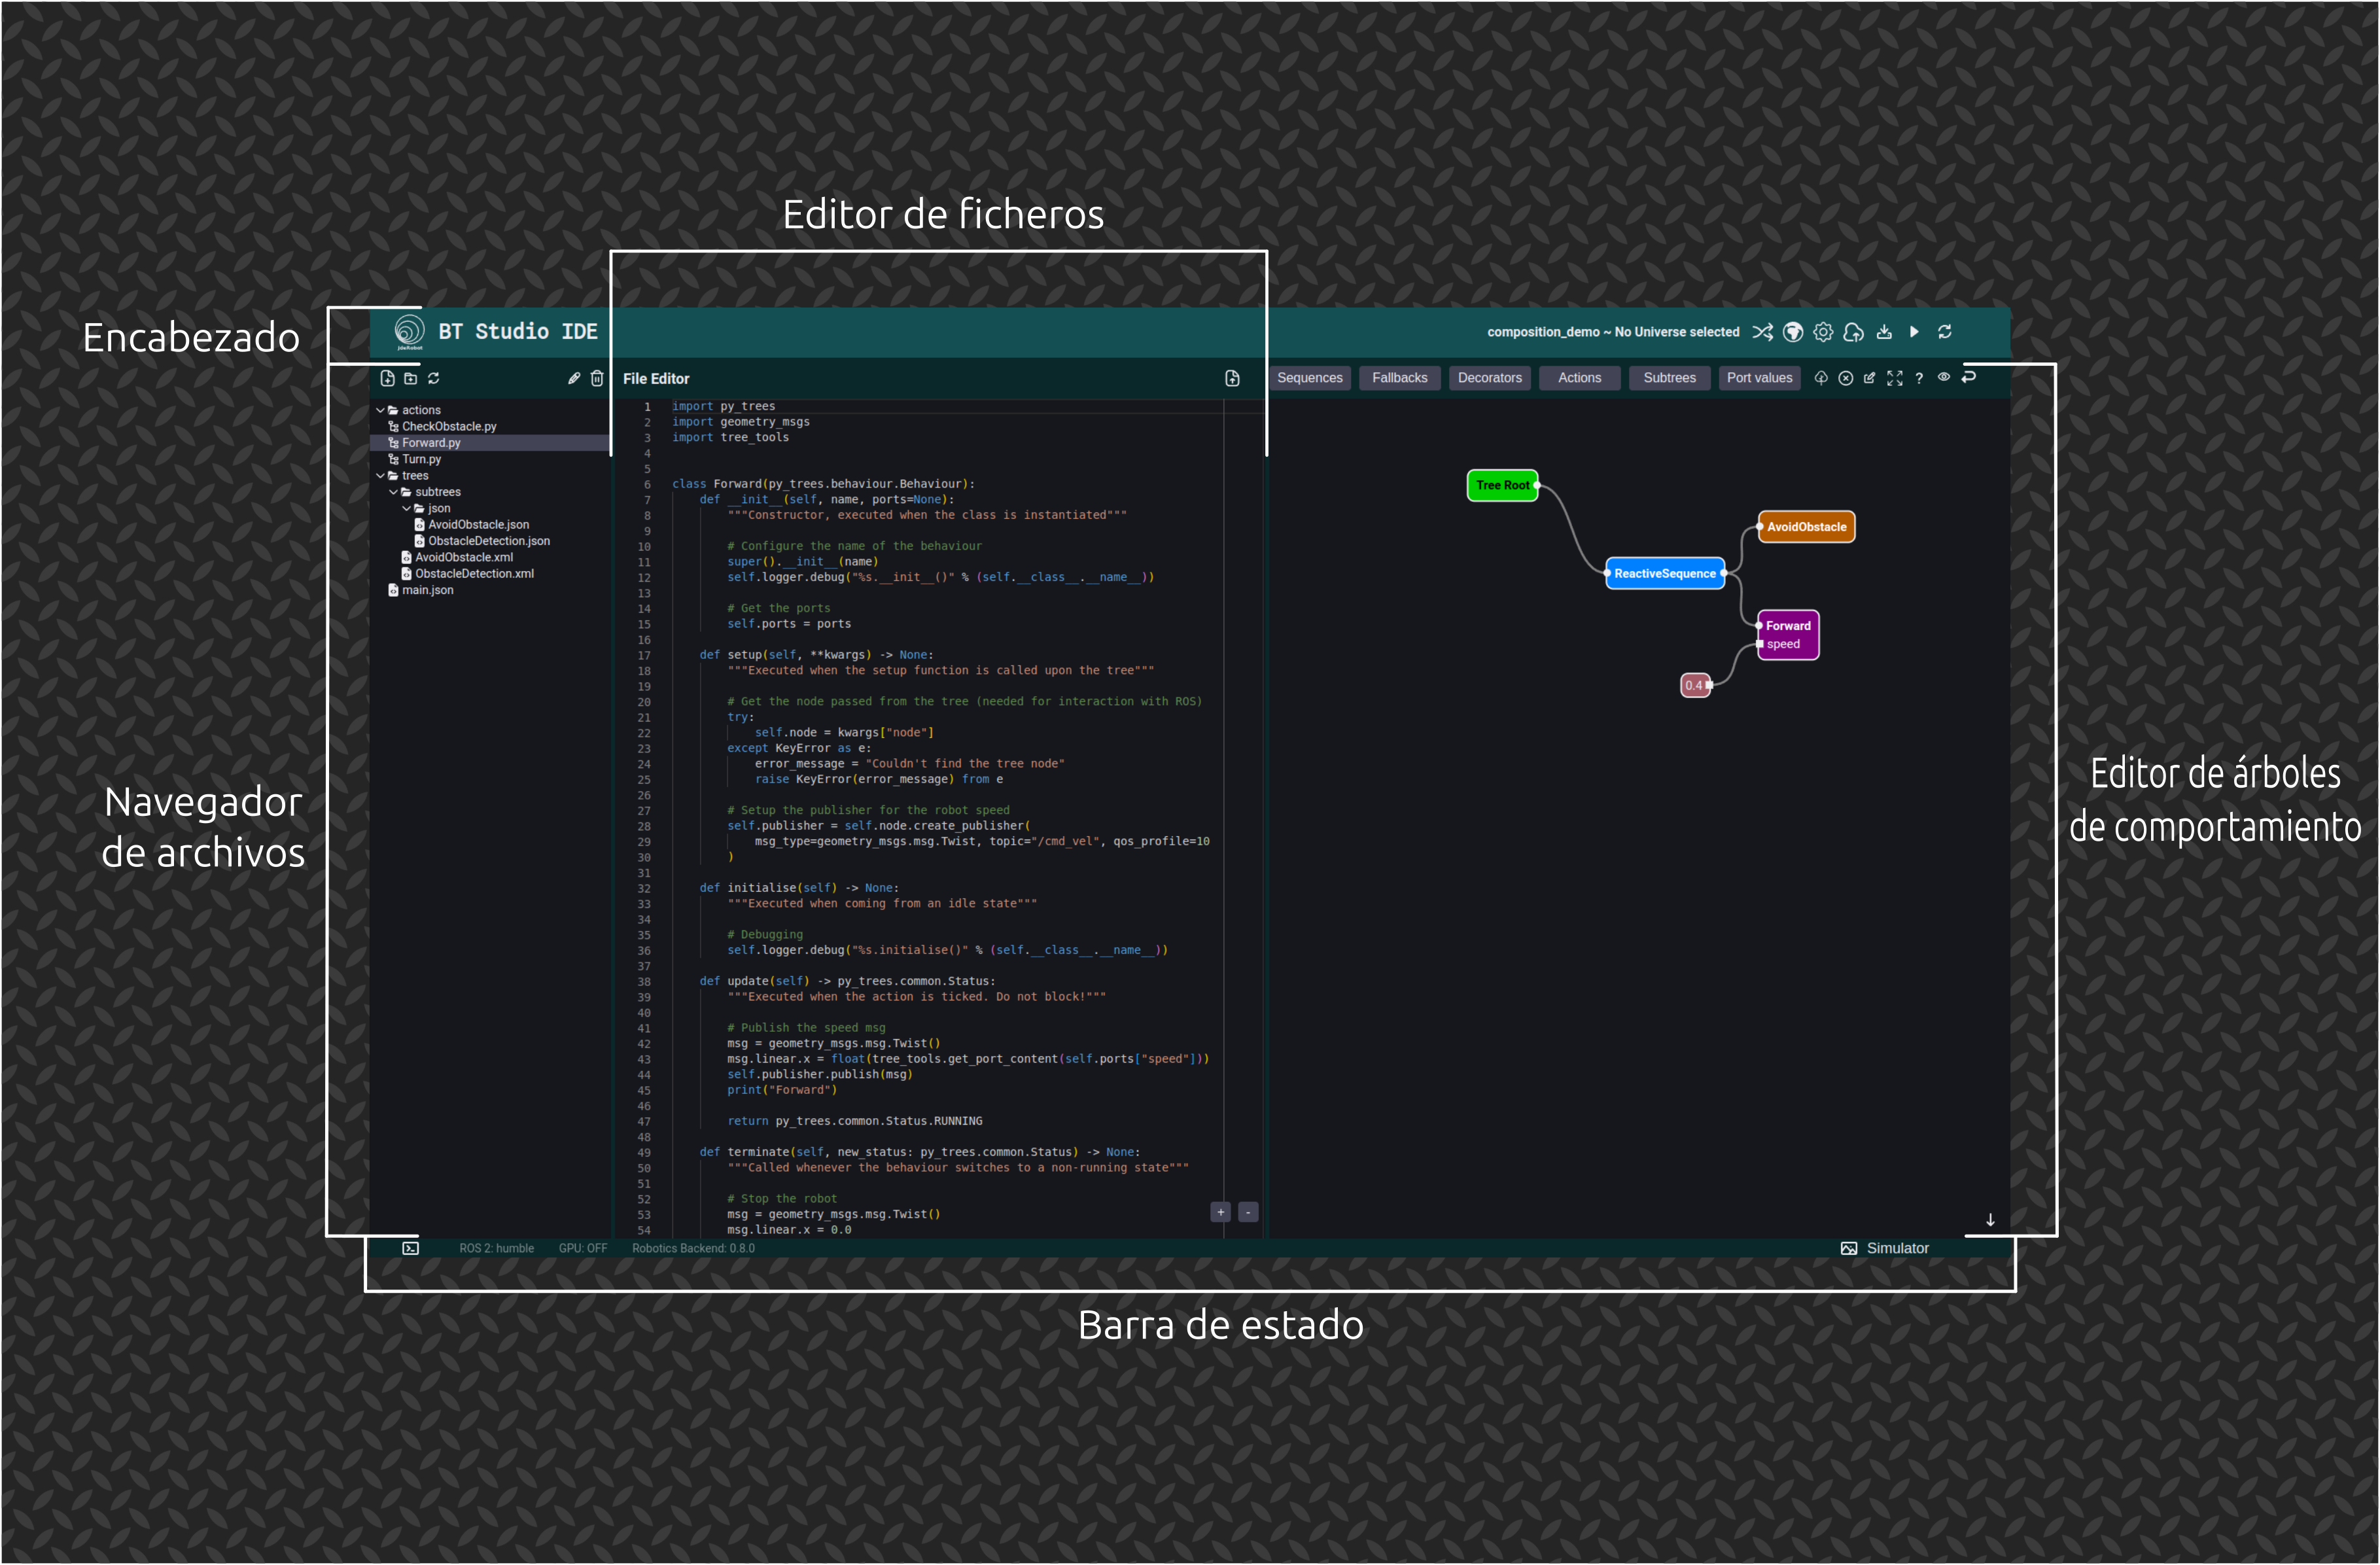
\includegraphics[width=\textwidth]{figures/bt-avances/bt-tetxo.png}
    \caption{Nueva interfaz gráfica de BT Studio sin ejecución}
    \label{fig:bt-int}
\end{figure}

Y cuando se está ejecutando la aplicación robótica en el entorno dockerizado aparecen los 2 visores que modifican la interfaz hasta parecerse a:

\begin{figure}[H]
    \centering
    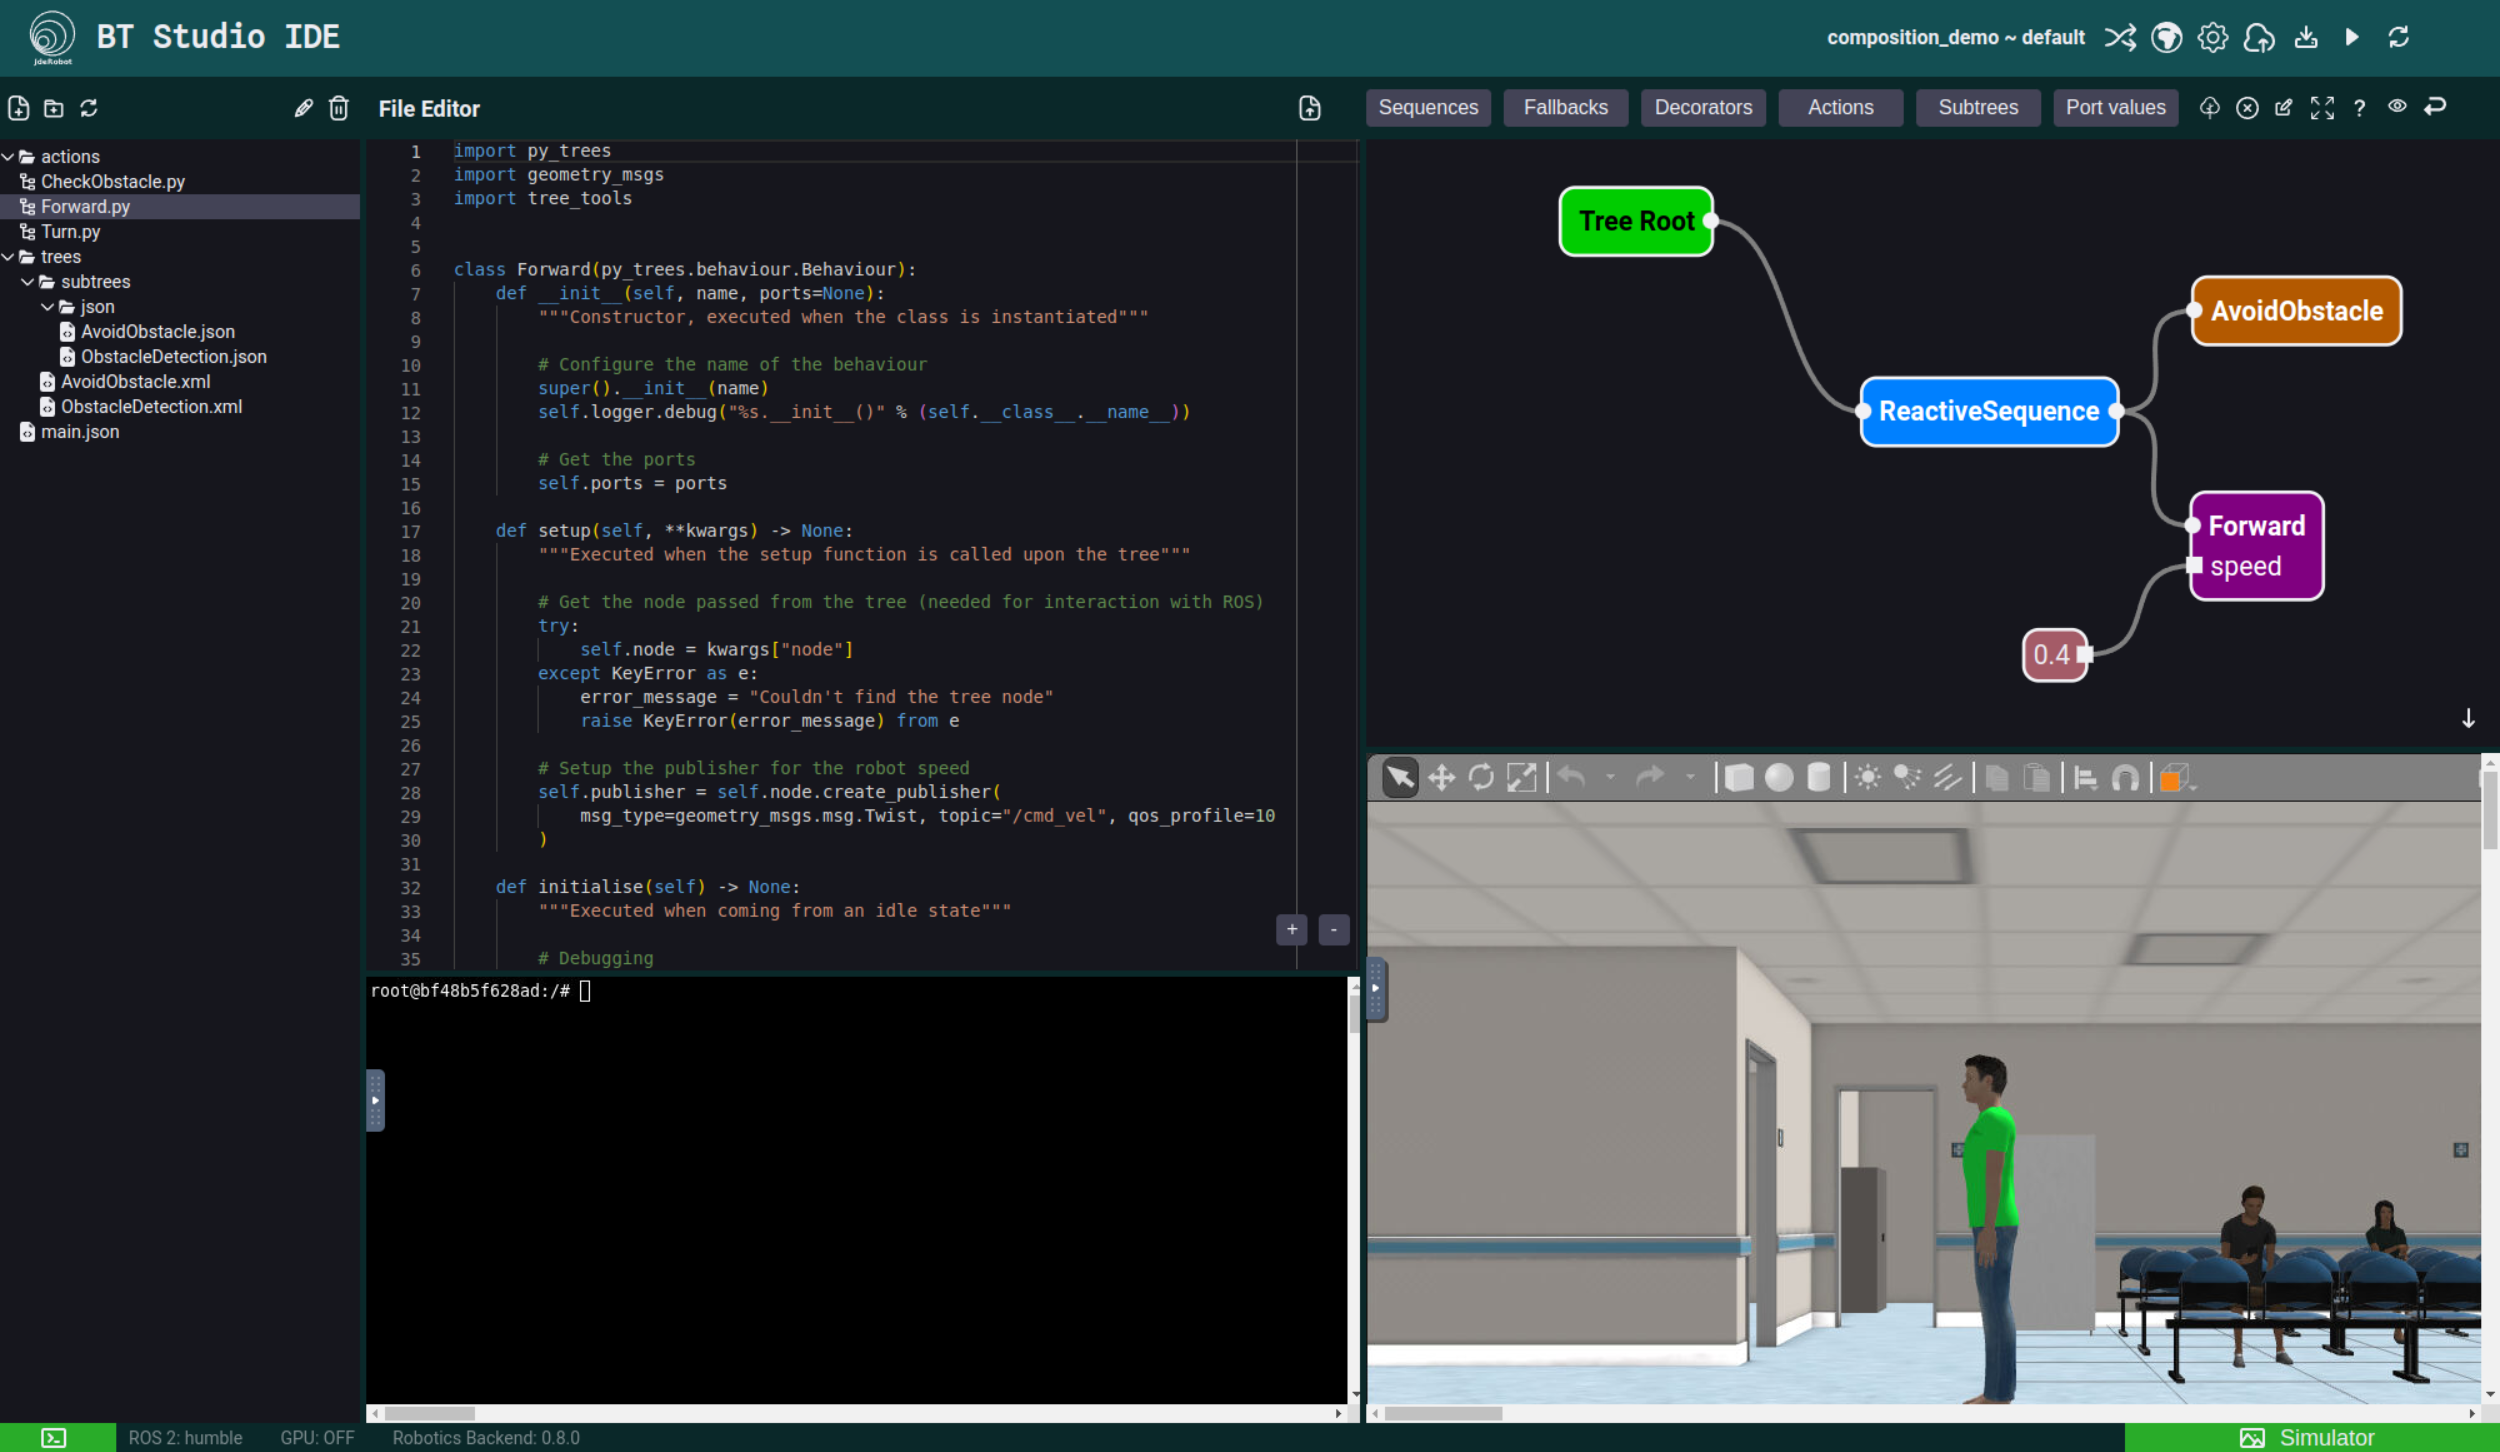
\includegraphics[width=\textwidth]{figures/bt-avances/bt-new-exec.png}
    \caption{Nueva interfaz gráfica de BT Studio en ejecución}
    \label{fig:bt-int-exec}
\end{figure}

A todos estos cambios, hay que sumarle también la posibilidad de cambiar el tema del web IDE a modo claro, que no estaba disponible en el antiguo BT Studio.

\subsection{Mejora del editor de árboles de comportamiento}\label{sec:bt-tree}

El editor de árboles de ejecución no ha quedado fuera de mejoras. Estas se pueden dividir en dos tipos: visuales y funcionales.

Las mejoras visuales corresponden a las realizadas con el fin de mejorar la apariencia del editor. Estas han sido las siguientes:

\begin{itemize}
    \item Cambio del color del fondo del editor para asemejarse al fondo del editor de ficheros y el navegador.
    \item Redondeo de los nodos del editor.
    \item Cambio del color del borde de las acciones para asemejarse al color de las letras.
    \item Cambio de los colores de los desplegables con los posibles nodos para asemejarse al resto del web IDE.
\end{itemize}

En cuanto a las mejoras funcionales, las siguientes son las que añaden algún tipo de funcionalidad nueva al editor. 

La primera y más básica de todas ellas es la prohibición de enlaces sueltos en el editor visual. Esto soluciona los problemas que se producían cuando se intentaba ejecutar una aplicación con un enlace que parecía estar conectado, pero no era el caso. Esto proporciona al usuario la confianza en que el árbol de comportamiento es tal y como se muestra para el usuario.

La segunda consiste en la adición de nuevos botones y el remplazo de otros existentes. En el primer caso, se han añadido tres nuevos botones que dan las siguientes funcionalidades: hacer zoom para centrar el árbol de comportamiento, ir a la documentación y cambiar entre el editor y el monitor de ejecución. En el otro caso, se han reemplazado los botones para añadir entradas y salidas a las acciones por uno para abrir el editor de acciones y etiquetas.

La tercera es la adición de la posibilidad de modificación del orden de ejecución del árbol de comportamiento. Esto es indicado por una flecha en la esquina inferior derecha y puede ser cambiada en el modal de configuraciones.

La cuarta modificación ha afectado a la hora de añadir múltiples instancias de una misma acción el árbol de comportamiento. Anteriormente, al añadir una nueva acción en el editor, esta se creaba sin ninguna entrada o salida, aunque hubiera una copia de esa acción ya cargada y esta tuviera alguna. Esto también ocurría al modificar las entradas y salidas de una de ellas. Para solucionar esto, ahora se guarda la información sobre todas las acciones del árbol y cuando una de estas se edita, se actualizan el resto de instancias de la acción. Esto es igual cuando se añade una copia de esa acción.

La última, al ser más compleja, se divide en los dos siguientes apartados:

\subsubsection{Editor de acciones}

Como su nombre indica, la utilidad de este es editar las acciones de una forma visual y sencilla para el usuario. Gracias a la cuarta mejora explicada anteriormente, todos los cambios a una acción se actualizarán en el resto de copias de esa acción inmediatamente. La funcionalidad que provee es la siguiente:

\begin{figure}[H]
    \centering
    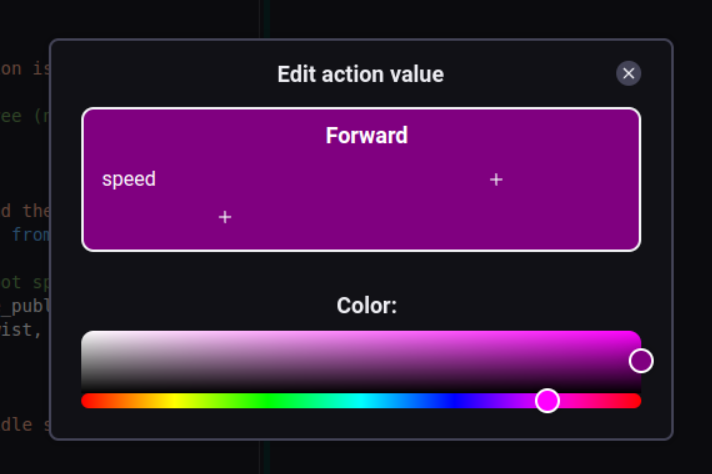
\includegraphics[width=0.5\textwidth]{figures/bt-avances/bt-edit.png}
    \caption{Editor de acciones}
    \label{fig:bt-act}
\end{figure}

\begin{itemize}
    \item Permite cambiar el color de la acción.
    \item Añadir puertos de entrada o salida siguiendo los siguientes pasos:
    \begin{enumerate}
        \item Presionar en el botón con el signo + en la columna correspondiente: izquierda para entradas y derecha para salida.
        \item Escribir el nombre del puerto.
        \item Si el nombre es válido aparecerá un botón verde para confirmar la creación del puerto, si no, solo aparecerá uno rojo para cancelarla.
        \item Presionar el botón verde para añadir el nuevo puerto.
    \end{enumerate}
    \item Borrar puertos de entrada o salida. Para esto es necesario presionar el botón rojo que aparece cuando el ratón se sitúa encima del puerto.
\end{itemize}

\subsubsection{Editor de etiquetas}

El editor de etiquetas tiene como función única permitir cambiar el contenido de la etiqueta. La única peculiaridad es que si la etiqueta se convierte a una etiqueta con acceso al \textit{blackboard}, definida en la sección \ref{sec:blackboard}, su color cambia para distinguirse de los normales en el editor.

\begin{figure}[H]
    \centering
    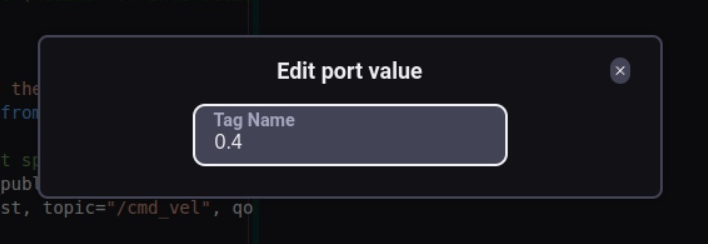
\includegraphics[width=0.6\textwidth]{figures/bt-avances/tag-edit.png}
    \caption{Editor de etiquetas}
    \label{fig:bt-tag}
\end{figure}

\subsection{Mejora del manejo de proyectos}

Se ha cambiado la forma de crear y navegar entre proyectos para que resulte más sencilla y visual al usuario. Los objetivos de esta mejora han sido los siguientes:

\begin{itemize}
    \item Substitución del \textit{popup} genérico del navegador por un modal con la lista de los proyectos creados.
    \item Reemplazar el \textit{popup} genérico del navegador por un modal para crear nuevos proyectos
    \item Permitir borrar proyectos.
\end{itemize}

Todo esto ha sido creado dentro de un solo componente, \textit{ProjectModal}, que se encuentra en el fichero \textit{frontend/src/components/header\_menu/modals/ProjectModal.tsx}. Este siempre se muestra al iniciar BT Studio, forzando al usuario a elegir un proyecto para continuar, ya que el modal no se puede cerrar si no hay un proyecto en activo.

\begin{figure}[H]
    \centering
    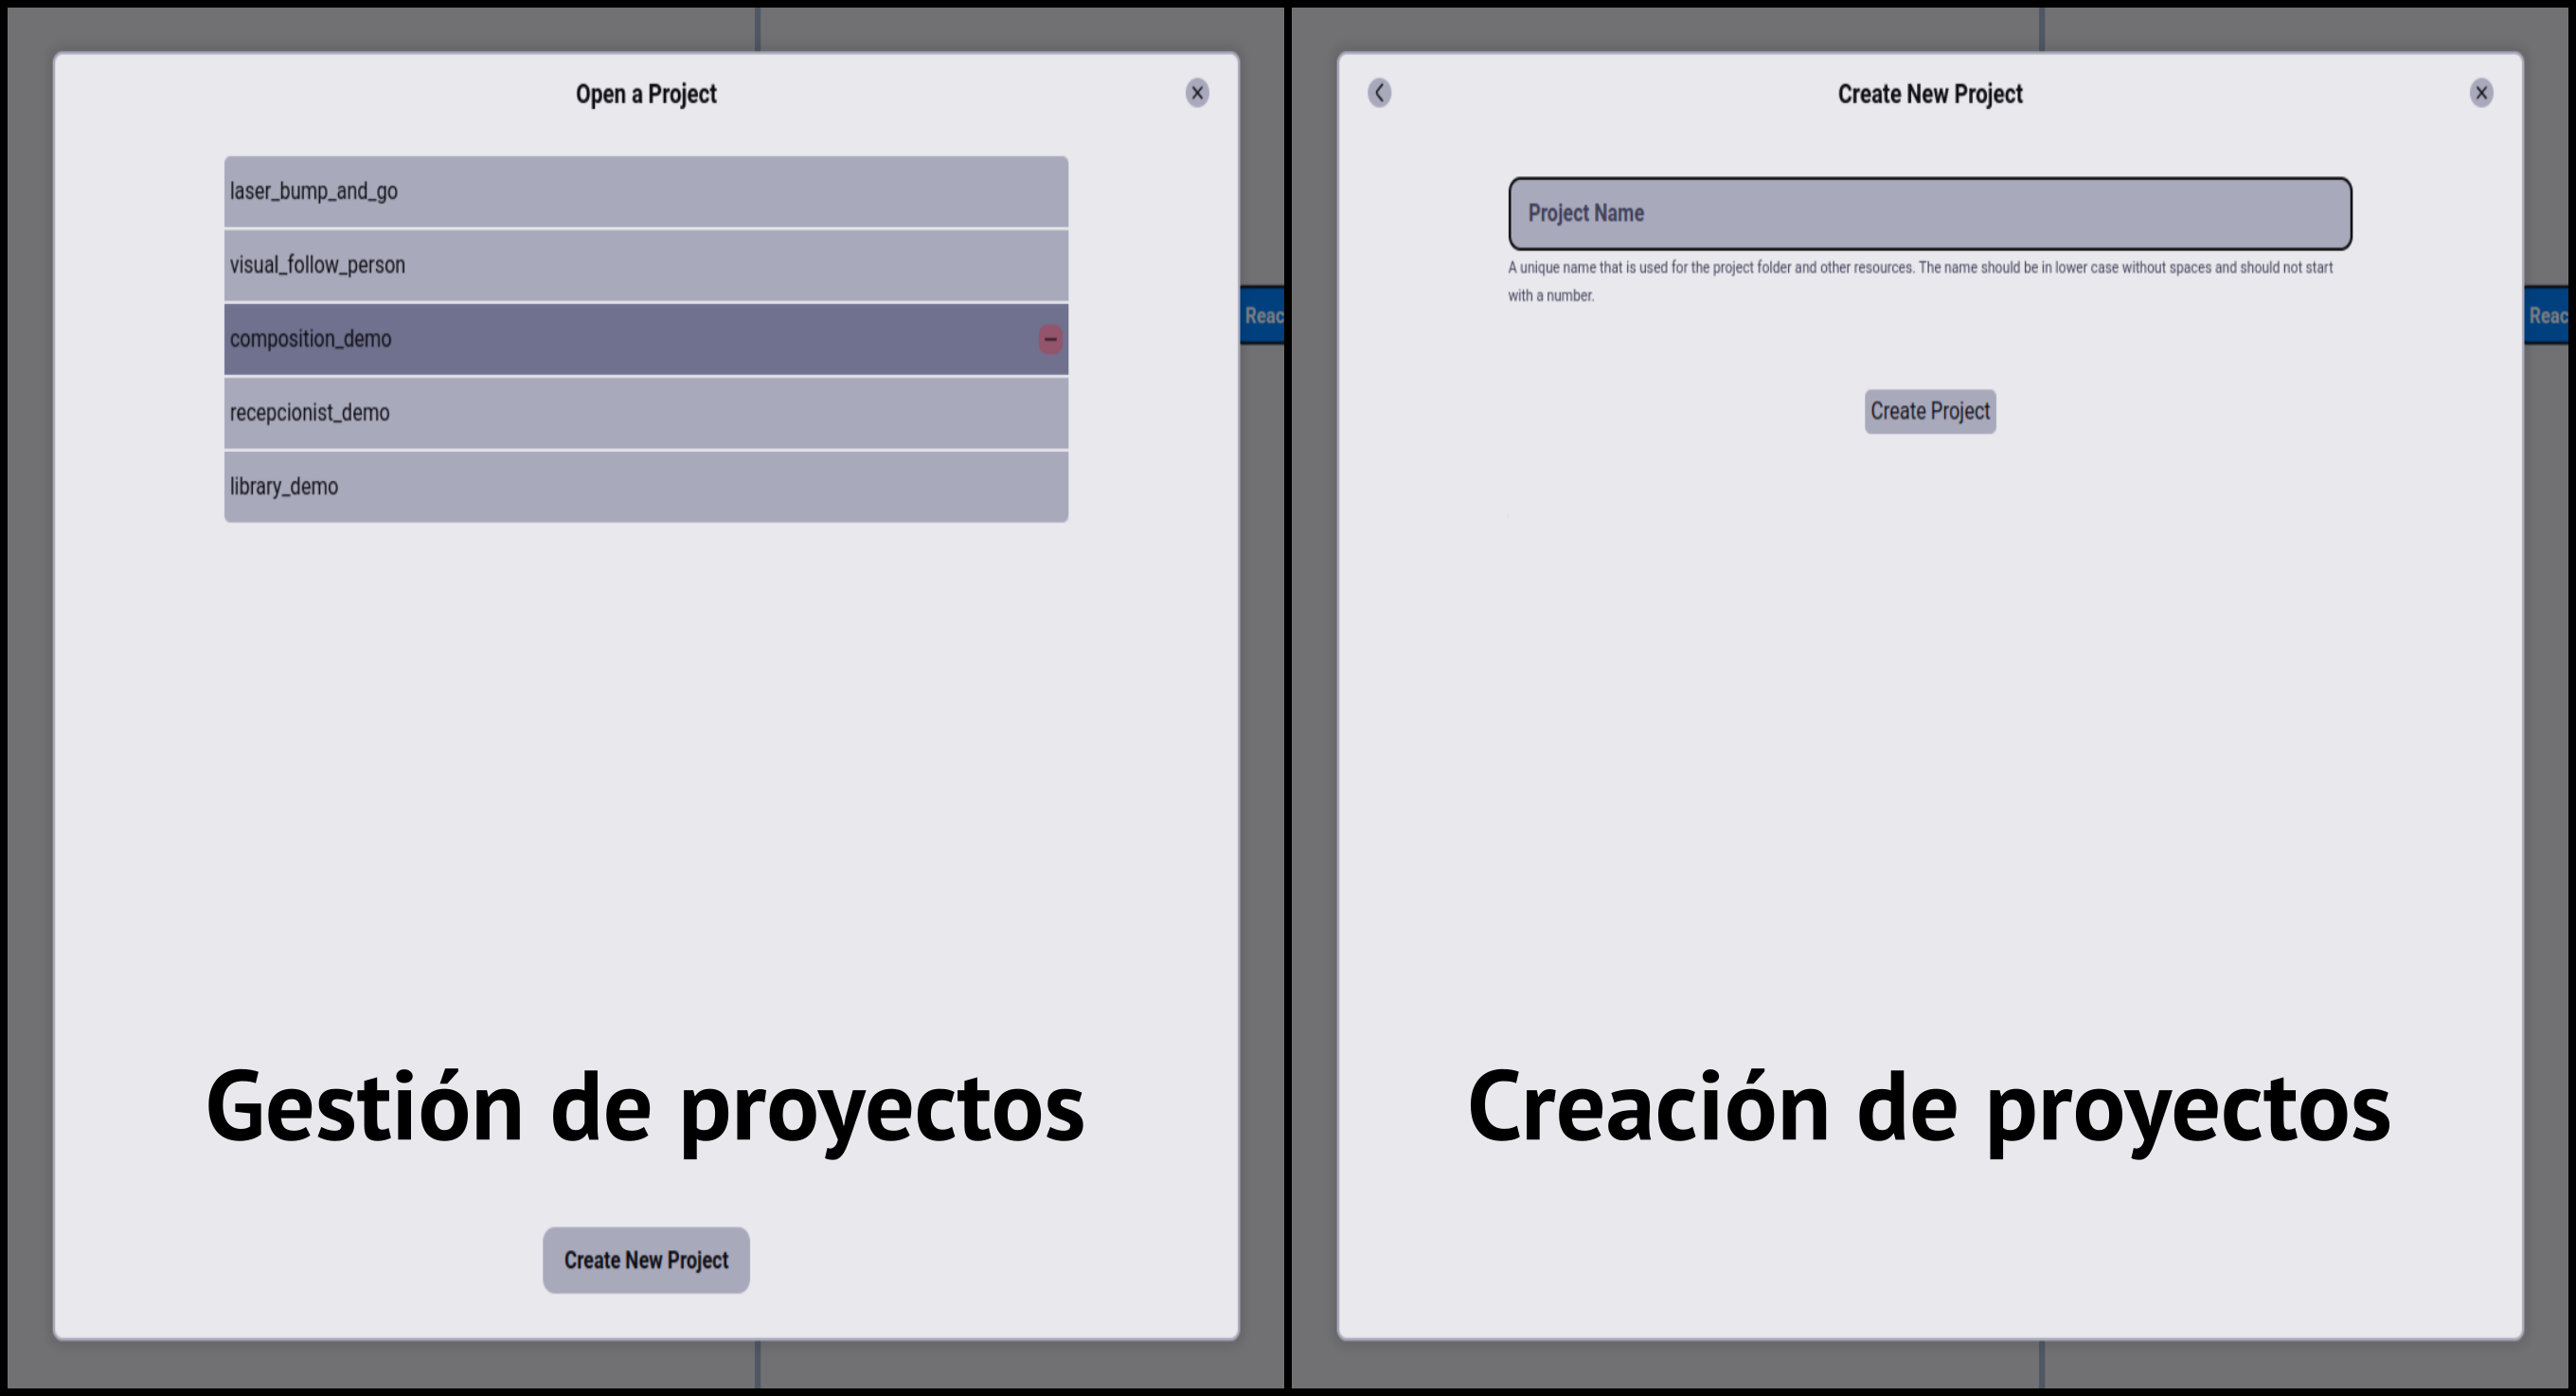
\includegraphics[width=\textwidth]{figures/bt-avances/bt-proy-2.png}
    \caption{Modales para gestión y creación de proyectos}
    \label{fig:proy-bar-rec}
\end{figure}

Al presionar encima de una de las entradas en la lista se seleccionará ese proyecto como activo y se cerrará el modal. Para poder borrar un proyecto se debe hacer clic en el botón rojo que se muestra al pasar el ratón por encima de la entrada correspondiente.

Cuando se desea crear un nuevo proyecto, después de presionar en el botón en la parte inferior del modal, este cambiará para mostrar un campo de entrada para introducir su nombre y un botón para confirmar la creación de este. 

% \begin{figure}[H]
%     \centering
%     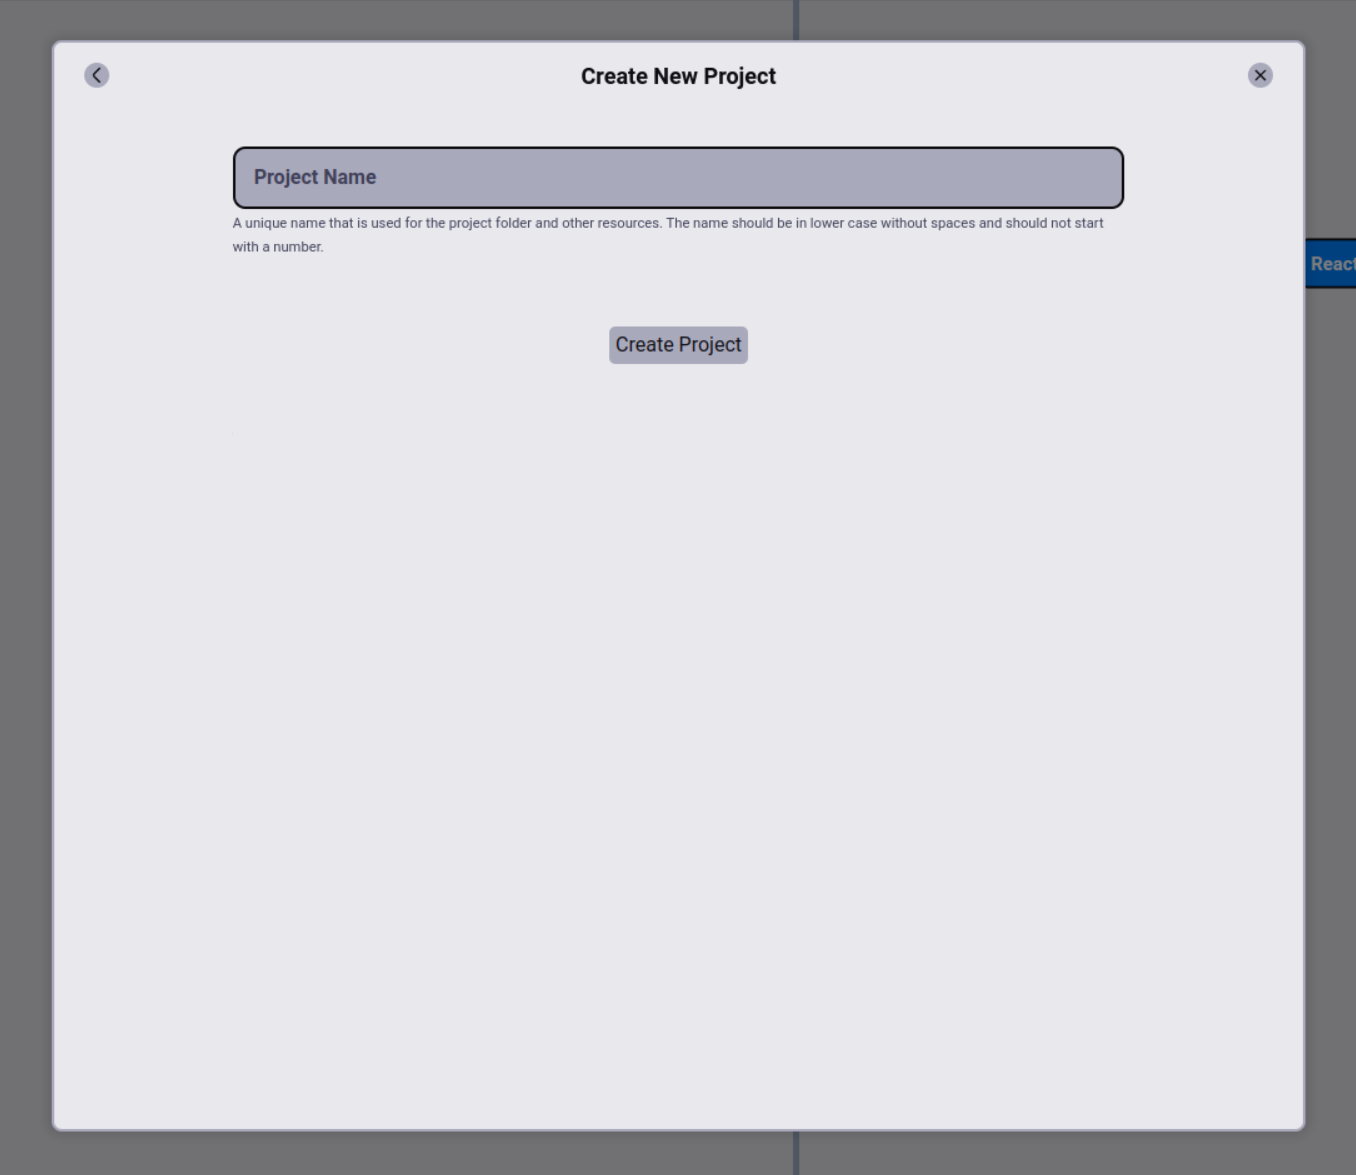
\includegraphics[width=0.5\textwidth]{figures/bt-avances/proj-create.png}
%     \caption{Apariencia del modal de proyectos}
%     \label{fig:status-bar-rec}
% \end{figure}

El modal usa los siguientes \textit{endpoints} del backend para realizar su funcionamiento:

\begin{itemize}
    \item \textbf{create\_project:} crea el nuevo proyecto.
    \item \textbf{get\_project\_list:} obtiene la lista de proyectos.
    \item \textbf{delete\_project:} borra el proyecto seleccionado.
\end{itemize} 

\subsection{Creación de la barra de estado}

La barra de estado tiene como objetivo mostrar al usuario el estado de la conexión con el entorno de ejecución dockerizado, ya sea BTDI o Robotics Backend, y permitir al usuario a forzar la conexión con este. Adicionalmente, posee un par de botones para controlar la visualización de los visores de ejecución, que se detallarán en la sección \textit{ejecución dockerizada}.

La barra de estado tiene dos estructuras diferentes dependiendo del estado de la conexión con el entorno de ejecución.

Este primero indica en naranja que no se ha podido realizar esa conexión.

\begin{figure}[H]
    \centering
    
\includegraphics[width=0.9\textwidth]{figures/bt-avances/status-bar-rec.png}
    \caption{Apariencia de la barra de estado sin conexión}
    \label{fig:status-bar-rec}
\end{figure}

Y, por otra parte, este al ya estar conectado, muestra la información sobre el entorno de ejecución.

\begin{figure}[H]
    \centering
    
\includegraphics[width=0.9\textwidth]{figures/bt-avances/status-bar.png}
    \caption{Apariencia de la barra de estado con conexión}
    \label{fig:status-bar}
\end{figure}

Para poder conseguir este funcionamiento se le deben pasar los siguientes \textit{props} al componente \textit{StatusBar} que se encuentra en el fichero \textit{frontend/src/components/status\_bar/StatusBar.tsx}:

\begin{itemize}
    \item \texttt{showSim}: indica si el visor del simulador está visible o no. 
    \item \texttt{setSimVisible}: función para cambiar la visibilidad en el visor del simulador.
    \item \texttt{showTerminal}: indica si el visor del terminal está visible o no. 
    \item \texttt{setTerminalVisible}: función para cambiar la visibilidad en el visor del terminal.
    \item \texttt{resetManager}: función para reiniciar el intento de conexión con el entorno de ejecución. Permite forzar la conexión cuando esta no es capaz de realizarse al primer intento. Cierra el intento de conexión activo del CommsManager (explicado en el capítulo \ref{cap:bt-studio}), borra el CommsManager activo, crea otra instancia y vuelve a intentar la conexión.
    \item \texttt{dockerData}: almacena la información sobre el entorno de ejecución dockerizada. 
\end{itemize}

\subsection{Mejora del editor}\label{sec:bt-monaco}

El editor de archivos ha sido reemplazado por completo, pasando de ACE \footnote{\url{https://ace.c9.io}} a Monaco \footnote{\url{https://microsoft.github.io/monaco-editor/}}. Este último es un editor creado por Microsoft y que es usado en el popular editor VS Code, pero que continúa siendo \textit{open source} bajo la licencia MIT.

\begin{figure}[H]
    \centering
    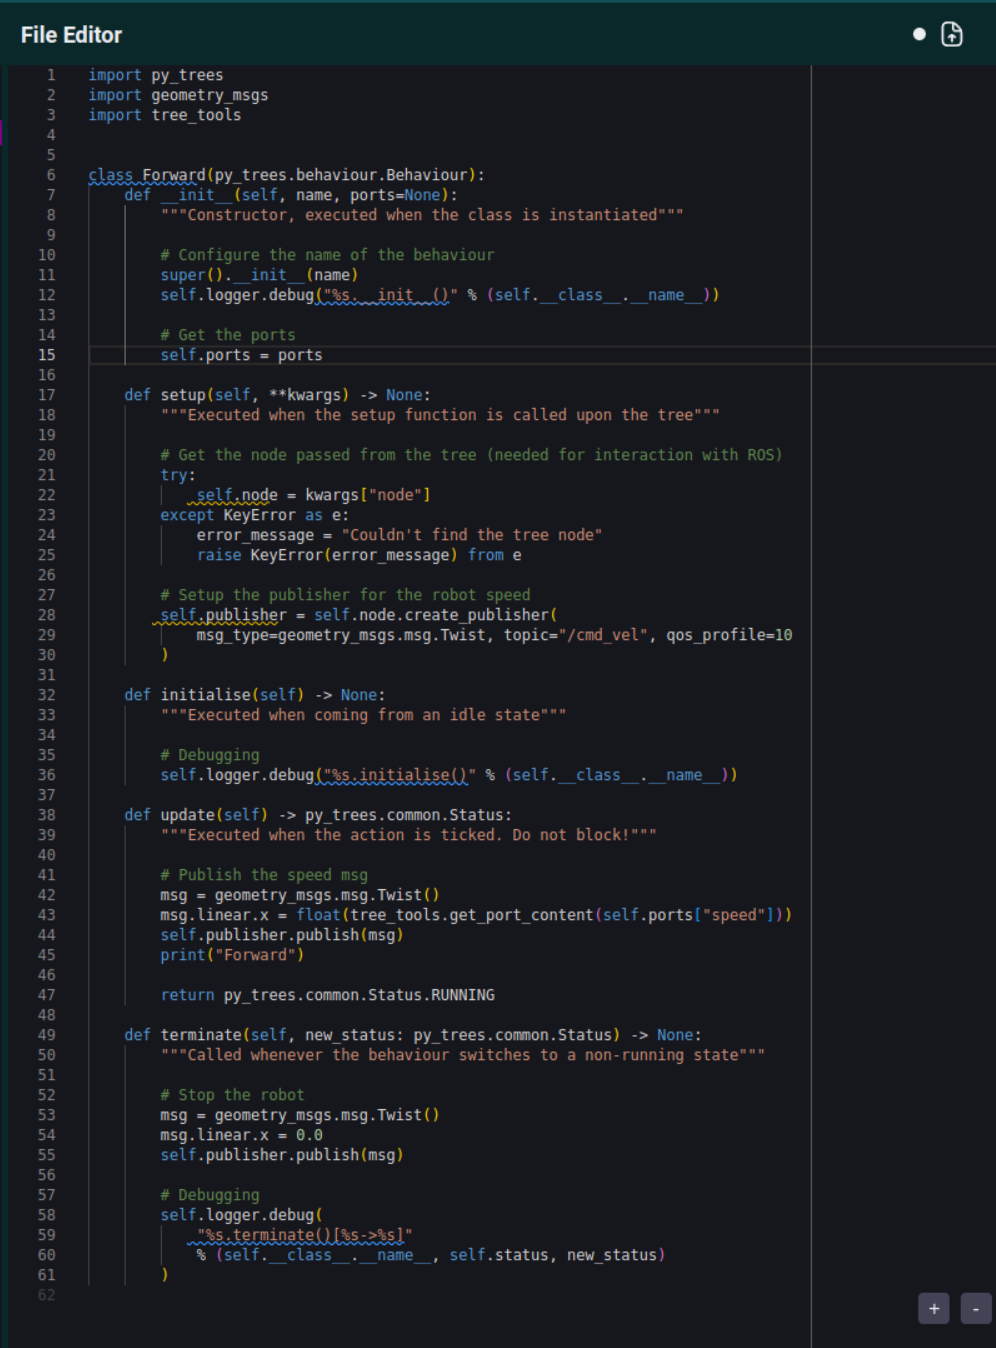
\includegraphics[width=0.6\textwidth]{figures/bt-avances/editor.png}
    \caption{Editor de archivos}
    \label{fig:bt-editor}
\end{figure}

Este nuevo editor ofrece una apariencia más moderna y varias mejoras de funcionalidad sobre ACE. Las que más interesan para BT Studio son las siguientes:

\begin{itemize}
    \item Soporte para búsqueda en el código usando \textbf{Ctrl + F}.
    \item Personalización más sencilla usando temas.
    \item Soporte para \textit{snippets} personalizados y autocompletado.
    \item Soporte para el resaltado de código para varios lenguajes de programación.
\end{itemize}

Gracias a todas estas funcionalidades se ha añadido al editor de BT Studio la capacidad de realizar las siguientes acciones siempre que se esté conectado al entorno de ejecución dockerizado gracias a la mediación del CommsManager, ya que este es capaz de intercambiar mensajes con el RAM donde se realiza el cómputo de todas las funciones que se van a detallar a continuación:

\begin{itemize}
    \item Formateo de código usando el formateador de Python. \textit{black}\footnote{\url{https://pypi.org/project/black/}}. Se activa desde el web IDE usando \textbf{Ctrl + Shift + I} y solo funciona para los ficheros de Python.
    \item Resaltado de código automático usando el \textit{linter} de Python \textit{pylint}\footnote{\url{https://pypi.org/project/pylint/}}. Solo funciona para los ficheros de Python. 
    \item Soporte para autocompletado de código usando \textit{jedi}\footnote{\url{https://pypi.org/project/jedi/}}, solo disponible para los ficheros de Python.
\end{itemize}

Todas estas funciones han sido añadidas desde este TFG en el Robotics Application Manager.

\subsection{Creación de \textit{popups}}

Para finalizar, la última mejora es la introducción de \textit{popups} para mostrar información al usuario que antes solo se encontraba en las trazas para desarrolladores. Estos han sido creados usando el mismo proceso que con las configuraciones, es decir, usando el elemento \textit{context} de React y envolviéndolo en un proveedor, \textit{ErrorProvider} que está localizado en el fichero \textit{frontend/src/components/error\_popup/ErrorModal.tsx}, y que se añade a la aplicación en el fichero \textit{frontend/src/index.js} para que esté disponible en toda la aplicación.

Con esto dicho, podemos pasar a mostrar cada uno de los tres tipos de \textit{popups}, así como su utilidad y forma de uso.

\subsubsection{\textit{Popup} de error}
\begin{itemize}
    \item Finalidad: mostrar al usuario que ha ocurrido un error. Se permite cerrar la ventana emergente sin problema.
    \item Forma de uso: usando la función \textit{error()} pasandole como parámetro el mensaje de error.
\end{itemize}
\begin{figure}[H]
    \centering
    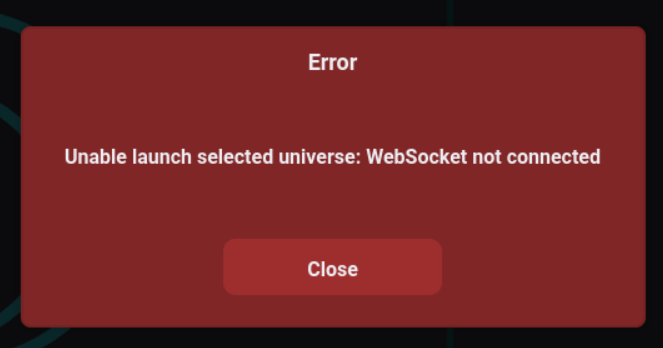
\includegraphics[width=0.55\textwidth]{figures/bt-avances/error.png}
    \caption{Popup de error}
    \label{fig:bt-err}
\end{figure}

\subsubsection{\textit{Popup} de error crítico}
\begin{itemize}
    \item Finalidad: mostrar al usuario que ha ocurrido un error y salir de la aplicación.
    \item Forma de uso: usando la función \textit{error\_critical()} pasandole como parámetro el mensaje de error.
    \item El aspecto es el mismo al de uno de error normal.
\end{itemize}

\subsubsection{\textit{Popup} de aviso}
\begin{itemize}
    \item Finalidad: mostrar al usuario que hay un aviso, normalmente porque algo no se está haciendo de forma correcta. Se permite cerrar la ventana emergente sin problema.
    \item Forma de uso: usando la función \textit{warning()} pasandole como parámetro el mensaje de error.
\end{itemize}
\begin{figure}[H]
    \centering
    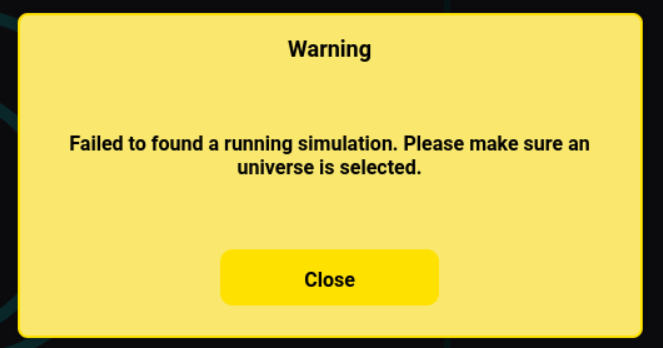
\includegraphics[width=0.55\textwidth]{figures/bt-avances/warning.png}
    \caption{Popup de aviso}
    \label{fig:bt-warn}
\end{figure}

\subsubsection{\textit{Popup} de información}
\begin{itemize}
    \item Finalidad: mostrar al usuario alguna información que no es ni un aviso ni un error. Se permite cerrar la ventana emergente sin problema.
    \item Forma de uso: usando la función \textit{info()} pasandole como parámetro el mensaje de error.
\end{itemize}
\begin{figure}[H]
    \centering
    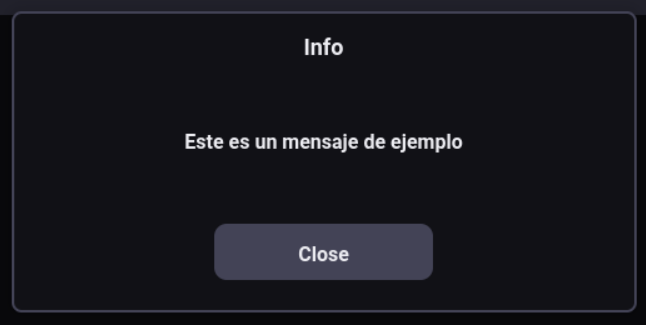
\includegraphics[width=0.55\textwidth]{figures/bt-avances/info.png}
    \caption{Popup de información}
    \label{fig:bt-info}
\end{figure}

\section{Navegador de archivos}

El navegador de archivos ha sido re-implementado completamente para adecuarse a un uso más generalizado y con más funcionalidad, ya que el editor antiguo solo podía crear acciones vacías y solo mostraba y dejaba eliminar estas acciones. Estos cambios permiten editar cualquiera de los ficheros de un proyecto, menos aquellos que se encuentran dentro del directorio \textit{trees}, debido a que cambios en estos pueden causar que se rompa el editor de árboles de comportamiento.

\begin{figure}[H]
    \centering
    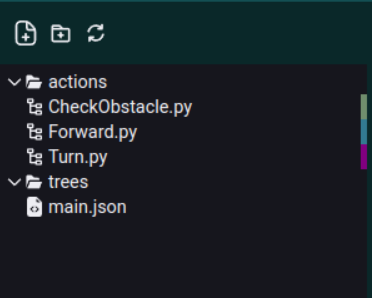
\includegraphics[width=0.3\textwidth]{figures/bt-avances/nav.png}
    \caption{Apariencia del navegador de archivos sin ninguno abierto}
    \label{fig:nav-close}
\end{figure}

El nuevo componente permite las siguientes funciones:

\begin{itemize}
    \item Mostrar todo el contenido del directorio \textit{code} del proyecto.
    \item Crear, renombrar y borrar ficheros.
    \item Crear, renombrar y borrar directorios.
    \item Crear acciones usando plantillas.
    \item Descargar ficheros o directorios.
    \item Subir ficheros al proyecto.
    \item Mostrar el color de la acción correspondiente del editor de árboles de comportamiento.
\end{itemize}

Para conseguir lo primero se ha implementado un navegador de ficheros que puede colapsar los directorios y que tabula los ficheros dentro de estos para poder visualizarlo de forma clara.

% \begin{figure}[H]
%     \centering
%     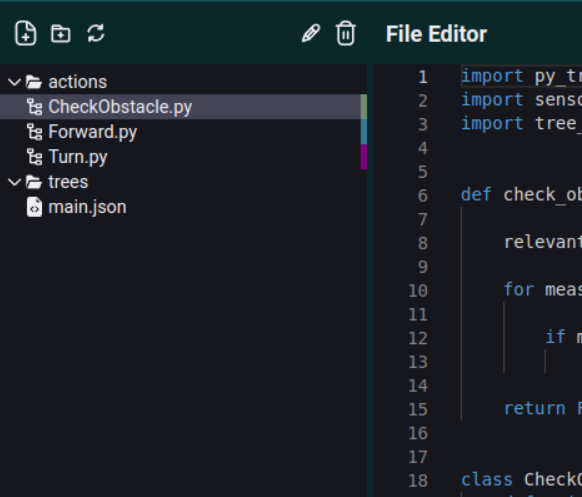
\includegraphics[width=0.4\textwidth]{figures/bt-avances/nav-open.png}
%     \caption{Apariencia del navegador de archivos con un fichero abierto}
%     \label{fig:nav-open}
% \end{figure}

En cuanto a los siguientes puntos, la mayoría de estos puede ser activados de dos maneras distintas: usando los botones disponibles en la parte superior del navegador o con el que aparece al mantener el ratón encima de esa entrada. Al hacerlo de esta última forma aparecerá un menú de contexto que tiene diferentes opciones dependiendo del fichero o directorio donde se ha activado.

\begin{figure}[H]
    \centering
    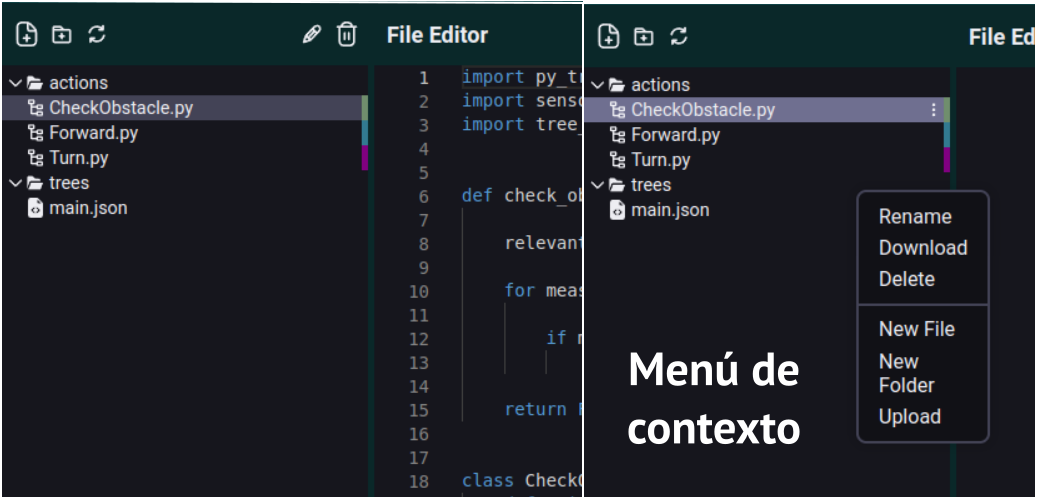
\includegraphics[width=\textwidth]{figures/bt-avances/bt-nav-2.png}
    \caption{Apariencia del menú de contexto del navegador de archivos}
    \label{fig:nav-menu}
\end{figure}

Todas las opciones disponibles abrirán un nuevo modal donde se podrán realizar la acción correspondiente, y si esta conlleva la creación o la subida de ficheros o directorios, se tendrá en cuenta la última entrada seleccionada en el modal para ser el lugar donde se lleve a cabo la acción. Estos modales son:

\subsubsection{Creación de ficheros y acciones}

Permite crear un fichero con el nombre escrito por el usuario. Solo si ese nombre es válido, es decir, no existe ya uno en ese lugar, se permite su creación.

\begin{figure}[H]
    \centering
    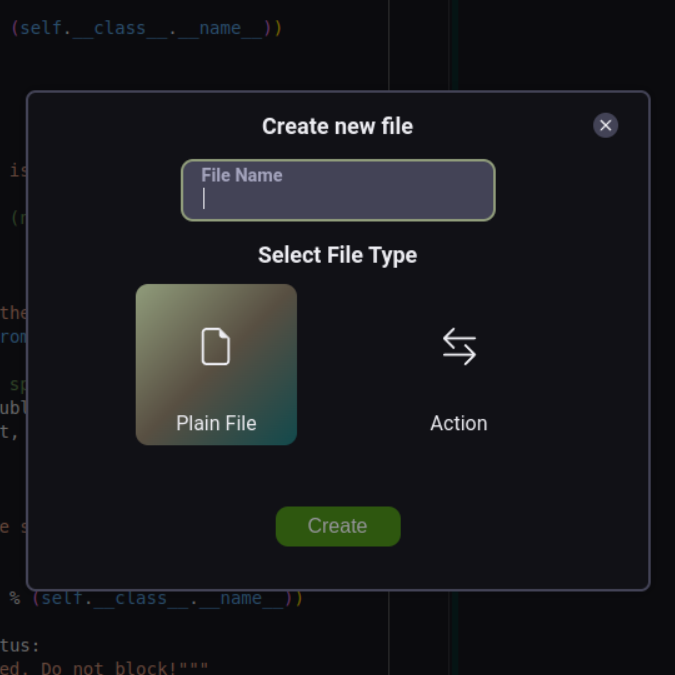
\includegraphics[width=0.5\textwidth]{figures/bt-avances/new-file.png}
    \caption{Modal de creación de ficheros}
    \label{fig:bt-file-new}
\end{figure}

Si se quiere crear una acción, es decir, un fichero de Python en un directorio especial, se debe primero seleccionar la opción de \textit{Acción} y luego seleccionar el tipo de plantilla que se desea: vacía, acción normal o acción con puertos. Como la acción siempre es un archivo de Python, se considera inválido su nombre, si además de lo definido anteriormente, posee algún punto o acaba en \textbf{.py}.

\begin{figure}[H]
    \centering
    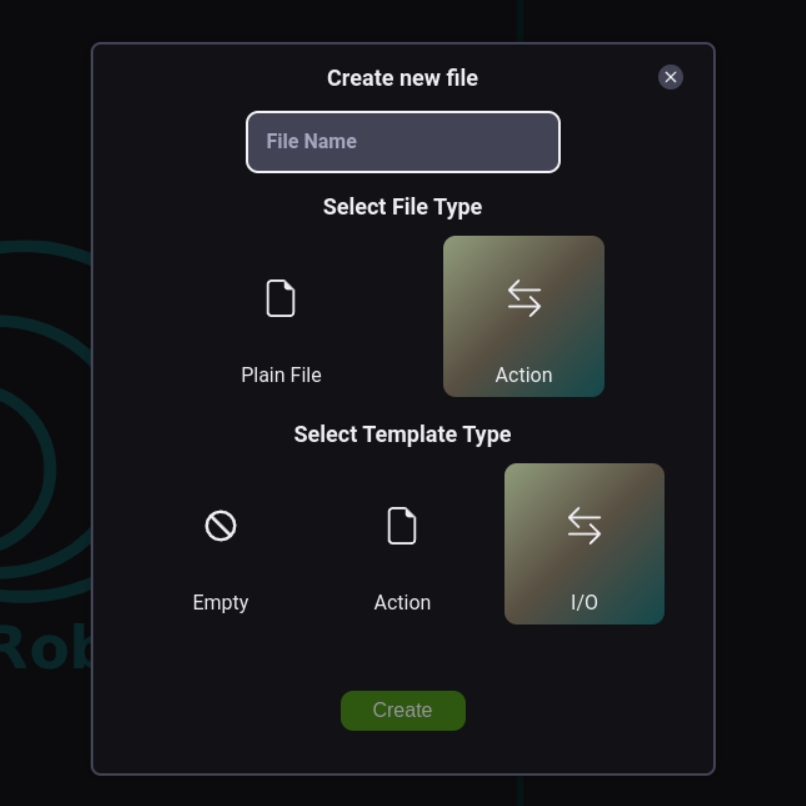
\includegraphics[width=0.5\textwidth]{figures/bt-avances/new-action.png}
    \caption{Modal de creación de acciones}
    \label{fig:bt-action-new}
\end{figure}

\subsubsection{Creación de directorios}

Permite crear un directorio con el nombre escrito por el usuario. Solo si ese nombre es válido, es decir, no existe ya en ese lugar, se permite su creación.

\begin{figure}[H]
    \centering
    \includegraphics[width=0.5\textwidth]{figures/bt-avances/bt-folder-new.png}
    \caption{Modal de creación de directorios}
    \label{fig:bt-dir-new}
\end{figure}

\subsubsection{Renombrar ficheros y directorios}

Permite renombrar un fichero o directorio con el nombre escrito por el usuario. Solo si ese nombre es válido, es decir, no existe ya en ese lugar, se permite renombrarlo.

\begin{figure}[H]
    \centering
    \includegraphics[width=0.5\textwidth]{figures/bt-avances/bt-rename.png}
    \caption{Modal de renombrar de directorios o ficheros}
    \label{fig:bt-rename}
\end{figure}

\subsubsection{Eliminar ficheros y directorios}

Muestra una ventana emergente para confirmar la eliminación del fichero o directorio seleccionado

\begin{figure}[H]
    \centering
    \includegraphics[width=0.5\textwidth]{figures/bt-avances/bt-del.png}
    \caption{Modal de eliminar directorios o ficheros}
    \label{fig:bt-delete}
\end{figure}

\subsubsection{Subir ficheros}

Permite subir ficheros desde el ordenador del usuario al proyecto

\begin{figure}[H]
    \centering
    \includegraphics[width=0.5\textwidth]{figures/bt-avances/bt-upload.png}
    \caption{Modal para subir ficheros}
    \label{fig:bt-upload}
\end{figure}

\section{Universos}

La adición de universos a BT Studio ha sido clave en la mejora de la experiencia del usuario a la hora de ejecutar las aplicaciones robóticas en el entorno dockerizado. La forma de cómo se lanza cada universo en el entorno dockerizado será explicado en su propia sección, \textit{ejecución dockerizada}. Antes de explicar esto en más detalle, se debe definir qué es un universo.

Se considera un universo a la combinación de un mundo y un robot, y en este caso en formatos que utiliza el simulador Gazebo. Estos universos deben tener además un punto de entrada para ser lanzados, y como se usa ROS2, este será un \textit{launcher}.

Con todo esto ya definido, el usuario tiene acceso a dos tipos de universos: los predefinidos en el Robotics Backend y los suyos personalizados. Para poder controlar y navegar entre los distintos universos se crea un nuevo modal que permite crear, eliminar y cambiar estos.

\begin{figure}[H]
    \centering
    \includegraphics[width=\textwidth]{figures/bt-avances/bt-univ.png}
    \caption{Modales para gestión y creación de universos}
    \label{fig:bt-univ}
\end{figure}

\subsection{Universos personalizados}

Para añadir un universo propio del usuario, este debe primero comprimir todos los ficheros que lo componen en un archivo ZIP y llamarlo con el nombre que quiere que aparezca en BT Studio. Por último, se debe presionar en el botón correspondiente en la esquina inferior izquierdo y subir el archivo del universo.

Estos universos solo tendrán soporte para la versión del simulador Gazebo, Harmonic.

\subsection{Universos del Robotics Backend}

Para poder utilizar estos universos en BT Studio se ha tenido que realizar un trabajo previo en Robotics Infrastructure (RI), Robotics Academy (RA) y en la propia forma de lanzar BT Studio. Esta última parte ya se ha explicado anteriormente en el apartado \ref{sec:uso-bt}.

El trabajo que se ha realizado en RI y en RA ha consistido primero en migrar las bases de datos de este último de SQLite a PostgreSQL con el objetivo de usar las mismas bases de datos que Unibotics, y posteriormente separar los universos en su propia base de datos y ubicarla en el repositorio de Robotics Infrastructure. Esto permitía usar la misma base de datos con los universos en Robotics Academy y en Unibotics, mejorando la experiencia del desarrollador y facilitando el mantenimiento.

El problema que surgía con estos cambios era que al usar PostgreSQL se necesita lanzar su propio servicio en un puerto del usuario y esto hacía que no fuera posible contenerlo todo dentro de un mismo contenedor docker. Para solucionarlo, se crea un nuevo contenedor basado en la imagen de PostgreSQL disponible en \textit{dockerhub} y gracias a la herramienta \textit{docker-compose} se lanzan los dos contenedores docker usando un solo fichero de configuración sin necesidad de instalar y correr PostgreSQL en local. Esto junto con la propiedad \textit{bind} de docker permite reemplazar el contenido de la base de datos con la que esté disponible en local, haciendo que el desarrollo de cambios en estas bases de datos sea sencillo para probar.

Pero con esto último volvía a aparecer otro problema, y era dónde situar la base de datos para que fuera cargada. Para esto se introdujo Robotics Infrastructure como submódulo en BT Studio y en Robotics Academy, ya que esto conseguía que la base de datos se mantuviera en un solo lugar, RI, pero se pudiera acceder a ella desde múltiples aplicaciones.

Con todo este trabajo previo ya realizado, ha hecho falta también adaptar la parte de Django de BT Studio para que entendiera y se conectará con el docker que contiene la base de datos de universos.

Ahora que BT Studio ya es capaz de acceder y mostrar las entradas de la base de datos de universos, al usuario se le muestra un campo de entrada para escribir el nombre del universo, y un desplegable para que elija entre la lista de los universos disponibles, como se muestra en la figura \ref{fig:bt-univ}.

Estos universos tienen soporte para las versiones del simulador Gazebo, Harmonic y Classic.

\section{Monitor de ejecución}\label{sec:bt-monitor}

La adición del monitor de ejecución provee al usuario de una manera visual y sencilla de observar el estado del árbol de comportamiento de la aplicación robótica. Este monitor está inspirado por el disponible en la aplicación \textit{Groot2} nombrada en la introducción y completa el objetivo restante de BT Studio, poseer de herramientas para la depuración de aplicaciones.

Este monitor se sitúa en el mismo lugar que el editor de árboles de comportamiento y se cambia de vista presionando el botón con forma de ojo que se halla presente en ambos. Para que el monitor de ejecución se haya podido crear, ha habido que trabajar en tres frentes distintos: el frontend, el backend y el entorno dockerizado.

\subsection{Backend}

En el backend ha hecho falta traducir el árbol de comportamiento a una lista con sus componentes simplificados, estando los nodos hijos contenidos como listas dentro de los padres. Esto ha sido posible gracias a la reutilización del traductor de JSON a XML ya existente, y que está explicado en más detalle en el TFG \cite{TFG_BT_Studio}, y un par de cambios. Gracias a este esqueleto generado se pueden situar los estados en las acciones adecuadas en el diagrama del monitor.

\subsection{Frontend}

Este recibe información de dos sitios para crear el diagrama final: del backend recibe el esqueleto del árbol y del entorno dockerizado recibe el estado actual de los nodos en todo momento. Todo esto, junto con el árbol de comportamiento original, permite mostrar sus estados de forma correcta en tiempo real.

Como el monitor de ejecución no debe permitir la edición del árbol de comportamiento, el diagrama mostrado no puede ser editado de ninguna manera, es decir, bloquea todo tipo de movimiento de nodos, su eliminación o su edición con los modales explicados en el apartado \ref{sec:bt-tree}.

\begin{figure}[H]
    \centering
    \includegraphics[width=0.8\textwidth]{figures/bt-avances/bt-monit.png}
    \caption{Apariencia del monitor de ejecución en una aplicación de ejemplo}
    \label{fig:bt-monit}
\end{figure}

Los nodos pueden mostrar cuatro estados distintos dependiendo de su ejecución:

\begin{itemize}
    \item Verde: el nodo ha acabado correctamente, devuelve \textit{Success}.
    \item Naranja: el nodo está ejecutándose, devuelve \textit{Running}.
    \item Rojo: el nodo ha fallado, devuelve \textit{Failure}.
    \item Gris: el nodo no se ejecuta.
\end{itemize}

\begin{figure}[H]
    \centering
    \includegraphics[width=0.5\textwidth]{figures/bt-avances/bt-monit-states.png}
    \caption{Estados de las acciones en el monitor de ejecución}
    \label{fig:bt-monit-state}
\end{figure}

Si una etiqueta tiene acceso al \textit{blackboard} esta tendrá su contenido actualizado, como se muestra en la imagen inferior.

\begin{figure}[H]
    \centering
    \includegraphics[width=0.5\textwidth]{figures/bt-avances/bt-tag-monit.png}
    \caption{Apariencia de una etiqueta con acceso al \textit{blackboard} en el monitor de ejecución}
    \label{fig:bt-tag-monit}
\end{figure}

\subsection{Entorno dockerizado}

Como se ha mencionado en el apartado anterior, el entorno dockerizado debe enviar el estado en el que se encuentra la aplicación en todo momento. Para conseguirlo ha hecho falta modificar el launcher de la aplicación robótica que BT Studio envía al entorno de ejecución, más detalle en la sección \ref{bt-studio:ejecutor}, para que este obtenga el estado de la aplicación, lo formatee y lo guarde en un fichero, y el RAM para que envíe a BT Studio los contenidos de ese fichero cada vez que cambie.

Lo primero se ha conseguido usando las funciones de PyTrees, \textit{py\_trees.display.ascii\_tree()} y \textit{py\_trees.display.ascii\_blackboard()}, para obtener el estado del árbol y del \textit{blackboard} respectivamente. Con estos estados, se ha definido en el fichero de Python \textit{tree\_tools}, que es usado en el lanzamiento de la aplicación, una función que traduce ese estado a un formato JSON que el frontend puede procesar. Y finalmente, con el estado traducido, este se escribe en un fichero de texto.

En la parte del RAM se ha añadido un servidor que envía el contenido del fichero usando WebSockets cuando este cambia. Estos mensajes son recibidos en BT Studio por el CommsManager que posteriormente se los entrega el monitor.

\section{Ejecución dockerizada}\label{bt-studio:ejecutor}

La última de las mejoras que afecta a la nueva funcionalidad de BT Studio es la ejecución dockerizada, que es un contenedor docker que proporciona un entorno con todas las herramientas necesarias para la visualización y ejecución de las aplicaciones. Este contenedor puede ser el Robotics Backend o el propio de BT Studio \footnote{\url{https://hub.docker.com/r/jderobot/bt-studio}} que contiene a ambos. El primero es usado cuando el web IDE no necesita ser lanzado, como en Unibotics, y el otro cuando se lanza de forma \textit{offline}.

De ahora en adelante, cuando se hable del Robotics Backend es como si fuera de ambos.

\begin{figure}[H]
    \centering
    \includegraphics[width=0.8\textwidth]{figures/bt-studio/docker_exec_detail.png}
    \caption{Ejecución de una aplicación robótica con el Robotics Backend}
    \label{fig:ejemplo}
\end{figure}

\subsection{Ejecución de aplicaciones}\label{sec:conex}

Cuando se lanza BT Studio, el \textit{CommsManager} intenta conectarse al puerto 7163. Este se queda esperando hasta que se lance el Robotics Backend, ya que el RAM dentro de este arranca un servidor Websocket en ese puerto, que permite la comunicación entre ambos. Una vez conectados, se podrán enviar comandos desde el frontend web del IDE al Robotics Backend y viceversa. Esto no es solo usado a la hora de ejecutar la aplicación, sino que también se utiliza para dar funcionalidad extra el editor.

A la hora de lanzar las aplicaciones, el Robotics Backend está dividido en cuatro pasos que deben realizarse de manera secuencial y monitorizada, al igual que los escalones de una escalera (Figura \ref{fig:radi_ladder}). Estos pasos están definidos por una máquina de estados interna al RAM, que abreviaremos como \textit{manager} para que sea más sencillo entenderlo.  

Esto implica que desde el frontend web de BT Studio se deben enviar los comandos correspondientes en el orden correcto para proceder con la ejecución. De manera secuencial, los cuatro mensajes para iniciar la ejecución son estos:

\begin{enumerate}
    \item \textbf{Connect}: abre la conexión con el servidor Websocket. El estado del \textit{manager} pasa a ser \textit{connected}. Esto ocurre cuando el \textit{CommsManager} se conecta al Robotics Backend.
     
    \item \textbf{LaunchUniverse}: envía un mensaje que contiene el universo que se desea lanzar, si este es de la base de datos se envía la información que se extrae de esta, y si es personalizado se envía un ZIP con todo el universo. En este paso se lanza el simulador de Gazebo, ya sea la versión Classic o Harmonic. El estado del \textit{manager} pasa a ser \textit{universe\_ready}. 
     
    \item \textbf{PrepareVisualization}: envía un mensaje con el tipo de visualización que requiere la aplicación. En el caso de BT Studio se crean dos visores VNC, uno para el simulador y otro para el terminal. Una vez creados, estos se conectan a sus contrapartes en el frontend web para poder visualizarlos. El estado del \textit{manager} pasa a ser \textit{visualization\_ready}. 
     
    \item \textbf{RunApplication:} se envía un ZIP que contiene la aplicación robótica. El \textit{manager} lo descomprime y lanza la ejecución desde el \textit{entrypoint} que es \textit{execute\_docker.py}. El estado del \textit{manager} pasa a ser \textit{app\_ready}.
\end{enumerate}

\begin{figure}[H]
    \centering
    \includegraphics[width=\textwidth]{figures/bt-studio/radi_ladder.png}
    \caption{Escalera de transiciones en el Robotics Backend durante la ejecución dockerizada de una aplicación robótica}
    \label{fig:radi_ladder}
\end{figure}

Durante toda esta secuencia, el \textit{manager} ejecuta los distintos componentes como subprocesos, lo que permite almacenar el PID de cada uno para posteriormente ejecutar varias acciones. Estas pueden variar dependiendo de los distintos componentes afectados: 

\begin{itemize}
    \item \textbf{Sobre la aplicación:}
    \begin{itemize}
        \item \textbf{Pause:} suspende la ejecución del proceso.
        \item \textbf{Resume:} continúa la ejecución del proceso.
        \item \textbf{TerminateApplication:} cierra  todos los procesos asociados a la ejecución de la aplicación. Además, reinicia y pausa la simulación en Gazebo. El estado del \textit{manager} pasa de \textit{application\_ready} a \textit{visualzation\_ready}. 
    \end{itemize}

    \item \textbf{Sobre la visualización:}
    \begin{itemize}
        \item \textbf{TerminateVisualization:} cierra todos los procesos asociados a la visualización, como el servidor VNC o el servidor que devuelve el estado del árbol de comportamiento. El estado del \textit{manager} pasa de \textit{visualzation\_ready} a \textit{universe\_ready}. 
    \end{itemize}

    \item \textbf{Sobre el entorno de simulación:}
    \begin{itemize}
        \item \textbf{TerminateUniverse:} cierra todos los procesos asociados a la ejecución del universo, especialmente el servidor de Gazebo. El estado del \textit{manager} pasa de \textit{universe\_ready} a \textit{connected}. 
    \end{itemize}
    
\end{itemize}

Gracias a todo esto, BT Studio permite al usuario elegir un universo de todos los predefinidos en el Robotics Backend o uno suyo propio, crear una aplicación robótica y ejecutarla en ese universo de forma repetitiva, sencilla y sin necesidad de instalación. También dota al usuario de la capacidad de control de la ejecución, al poder pararla o reiniciarla usando los botones disponibles en la esquina superior derecha de la interfaz.

\section{Integración en Unibotics}\label{sec:bt-unib}

Para finalizar, el último objetivo y el principal de esta mejora ha sido la integración total de BT Studio en la versión online de Unibotics. Esto se ha logrado de forma escalonada a lo largo del proyecto siguiendo las siguientes etapas:

\begin{enumerate}
    \item Añadir Robotics Infrastructure como submódulo de Unibotics.
    \item Modificar el lanzamiento de BT Studio para que este sea en un contenedor Docker.
    \item Añadir la ejecución dockerizada a BT Studio.
    \item Añadir BT Studio como submódulo de Unibotics.
\end{enumerate}

Como las tres primeras ya han sido contadas anteriormente, solo se va a explicar el proceso necesario para la última.

\subsection{BT Studio como submódulo}

Unibotics está compuesto de tres despliegues distintos, como se detalla en la sección \ref{sec:unibotics}: D1, D2 y D3. Para la integración se ha trabajado la mayoría del tiempo en D1 y los detalles finales en D2.

Comenzando con la integración, el primer paso fue conseguir compilar el frontend web de Unibotics en D1 con BT Studio. Esto resulto ser bastante laborioso debido a las múltiples configuraciones que hacía falta modificar en la configuración de Webpack, ya que había conflictos a la hora de tratar el código fuente de BT Studio al estar este en TypeScript y no en JavaScript como el resto de la plataforma.

Una vez que compilaba, lo siguiente era mostrarlo en el navegador correctamente. Para conseguirlo se tuvo que crear una nueva plantilla de HTML y un fichero de JavaScript en Unibotics para reemplazar el \textit{index.js} de BT Studio y que carga el resto del web IDE. Todo esto tenía como objetivo que Django reconociera cómo cargarlo, ya que este no es capaz de acceder a los ficheros situados en el submódulo de BT Studio. 

Una vez se consiguió esto, hubo múltiples problemas por las clases de CSS, ya que Unibotics sobrescribía las propias de BT Studio. Para solucionarlo hizo falta renombrarlas, todas añadiendo \textbf{bt-} al inicio de sus nombres. 

Lo último que tuvo lugar en D1 fue la copia del backend web de BT Studio al directorio situado dentro de Unibotics donde se encontraba la carpeta con el de Robotics Academy, que había sido integrado como submódulo anteriormente. Una vez el backend situado en su sitio y funcionando correctamente con los ficheros locales, se pasó al trato de archivos en remoto.

Los proyectos robóticos del usuario en BT Studio, sus archivos, cuando está integrado en Unibotics se almacenan en la nube de Amazon. Esto requiere de esa nube ya en el uso del despliegue D2 de Unibotics que además asegura que el funcionamiento va a ser igual que en el despliegue de producción D3. Estos archivos se encuentran en un servidor corriendo Amazon Simple Storage Service (Amazon S3) que ofrece un SDK o \textit{Software Development Kit} para interactuar con ellos a través del paquete de Python \textit{boto3}. Usando esto, se han replicado varias funciones que acceden a ficheros como:

\begin{itemize}
    \item \textit{aws\_pull\_ide\_file}: devuelve el contenido de un fichero.
    \item \textit{aws\_push\_ide\_file}: guarda el contenido a un fichero o si este no existe lo crea.
    \item \textit{aws\_exists\_ide\_file}: devuelve si el fichero existe.
    \item \textit{aws\_push\_ide\_folder}: crea un directorio vacío. Como en S3 no hay directorios, lo único que hace es añadir un objeto vacío con ese nombre.
    \item \textit{aws\_delete\_ide\_file}: elimina un fichero.
    \item \textit{aws\_delete\_ide\_folder}: elimina un directorio y sus contenidos de forma recursiva.
    \item \textit{aws\_rename\_ide\_file}: renombra un fichero.
    \item \textit{aws\_rename\_ide\_folder}: renombra un directorio.
    \item \textit{aws\_get\_filenames}: devuelve un listado con los nombres de los ficheros o directorios dentro de la carpeta especificada.
    \item \textit{aws\_get\_user\_projects}: devuelve una lista con todos los proyectos de un usuario.
    \item \textit{aws\_get\_user\_project\_universes}: devuelve una lista con todos los universos de un proyecto.
    \item \textit{aws\_create\_empty\_project}: crea un proyecto vacío en el directorio correspondiente al usuario: \textit{bt\_studio/NOMBRE\_USUARIO}.
    \item \textit{aws\_delete\_project}: elimina un proyecto y todos sus contenidos.
    \item \textit{aws\_create\_bt\_docker\_universe}: crea la entrada para un universo definido en el Robotics Backend.
\end{itemize}

Todas estas funciones se añaden a las funciones que componen el backend de BT Studio acompañadas de una declaración condicional que usa el acceso normal, local, si el despliegue es D1 y el acceso con S3 si es D2 o D3.

\subsection{Funcionalidad modificada}

Ha habido varios aspectos de BT Studio que se han tenido que restringir debido al peligro que podían causar a la estabilidad de la plataforma Unibotics. Debido a que Unibotics utiliza un solo servidor, se ha intentado aliviar el coste computacional del backend web sobre este. Esto ha obligado a mover toda la creación de archivos ZIP desde el backend web al frontend web que ha afectado gravemente a estas 3 funcionalidades:

\begin{itemize}
    \item La creación de la aplicación robótica: tanto para descarga local como para la ejecución dockerizada se ha migrado toda la creación del ZIP al frontend web conservando toda la funcionalidad.
    \item Los universos personalizados: no se ha conseguido mover la creación del ZIP, lo que causa que solo esté disponible por ahora en la versión \textit{offline}.
    \item La subida de código local: no se ha conseguido migrar la descompresión del ZIP, por lo que solo está disponible en la versión \textit{offline}.
\end{itemize}
    \chapter{Validación experimental}\label{cap:validacion}

En este capítulo se muestran los resultados de la validación experimental de los objetivos expuestos en el capítulo \ref{cap:planificación}. Se explicarán detalladamente los procedimientos seguidos para el desarrollo de las tres aplicaciones robóticas de ejemplo.

\section{Procedimiento experimental y verificación de funcionalidad}

El procedimiento seguido para la validación experimental consiste en el desarrollo de las tres aplicaciones roboóticas de ejemplo utilizando exclusivamente BT Studio y usando el entorno de ejecución integrado. El proceso de creación de las aplicaciones robóticas es el mismo para todas ellas y este puede ser visto en el siguiente video: \url{https://youtu.be/0kK68lDe_Vo}.

Estas aplicaciones muestran el correcto funcionamiento de las siguientes funcionalidades de BT Studio creadas a lo largo de este TFG:

\begin{itemize}

    \item Acceso desde cualquier navegador tras la instalación en local de BT Studio, desde el contenedor de docker de BT Studio \footnote{\url{https://hub.docker.com/repository/docker/jderobot/bt-studio}} o desde la plataforma web de Unibotics usando el Robotics Backend. 

    \item Mecanismo para la gestión y navegación entre distintos proyectos robóticos. Cada proyecto almacena una sección donde se guardan el conjunto de acciones y árboles de comportamiento, y otra donde están los universos pertenecientes al mismo. 

    \item Mecanismo para la gestión y navegación entre distintos universos. Estos pueden ser los que vienen predefinidos en el Robotics Backend o personalizados. 
    
    \item Edición de ficheros Python para la programación acciones de un árbol de comportamiento. Además, si está conectado a un contenedor docker que contiene el Robotics Backend, como el contenedor de BT Studio, se le añade la funcionalidad de autocompletado, resaltado de sintaxis y formateo de  código en los ficheros de Python. 

    \item Creación de árboles de comportamiento mediante un editor visual basado en bloques (ya estaba en la versión de partida de BT Studio). Permite la creación de BT compatibles con el estándar definido en BT.cpp, el uso de acciones definidas por el usuario y su personalización.

    \item Integración con el Robotics Backend para la ejecución de las aplicaciones programadas por los usuarios. 
    
    \item Mecanismos para el control y visualización de la ejecución de las aplicaciones desde el navegador, así como la monitorización del estado de los árboles de comportamiento. 
    
\end{itemize}

Se desarrollaron tres aplicaciones robóticas ilustrativas con la versión final de BTStudio
desarrollada en este TFG: \textit{Laser Bump and Go}, \textit{Follow Person} y \textit{RoboCup Receptionist}. Las dos primeras fueron mejoradas a partir de las versiones existentes, mientras que la última fue creada enteramente en la versión offline de BT Studio desarrollada. Los videos fueron grabados en la versión offline, pero han sido replicados en el despliegue D1 de Unibotics y pueden ser reproducidos en el despliegue de producción de D3 de Unibotics.

\section{Aplicación: Laser Bump and Go}

Esta aplicación está basada en la disponible en la versión 0.3 de BT Studio, que consistía en que el robot vaya en línea recta hasta que encuentra un obstáculo y gira. Para la detección de obstáculos se usa un sensor láser a bordo del robot que es el turtlebot2.

También se muestra la composición de árboles de comportamiento que fue añadida por un proyecto del GSOC\footnote{\url{https://theroboticsclub.github.io/gsoc2024-Oscar_Martinez/}}.

\subsection{Resumen}

\begin{itemize}
    \item \textbf{Código para consulta:} \url{https://github.com/JdeRobot/bt-studio/tree/main/backend/filesystem/composition_demo}
    \item \textbf{Simulador:} Gazebo Classic.
    \item \textbf{Robot:} TurtleBot2.
    \item \textbf{Universo:} Hospital (Follow Person) del Robotics Backend llamado \textit{default} en BT Studio.
    \item \textbf{Sensores:} LIDAR 2D.
    \item \textbf{Sentido de ejecución:} de arriba hacia abajo. 
\end{itemize}

\subsection{Implementación en BT Studio}

\subsubsection{Listado de acciones}
\begin{itemize}
    \item \textbf{Forward:} obtiene la velocidad lineal deseada a través del puerto de entrada \textit{lin\_speed} y la publica a través del topic \textit{/cmd\_vel}. Cuando le llega un tick devuelve \textit{Running}. 
    \item \textbf{Turn:} obtiene la velocidad angular deseada a través del puerto de entrada \textit{ang\_speed} y la publica a través del topic \textit{/cmd\_vel}. Cuando le llega un tick devuelve \textit{Running}. 
    \item \textbf{CheckObstacle:} se suscribe al topic \textit{/scan} donde se publican las medidas del láser. Cuando le llega un tick, si las medidas del láser dentro de la amplitud deseada que obtiene a través del puerto de entrada \textit{amplitude} son menores que la distancia mínima indicada en el puerto de entrada \textit{obs\_dist} devuelve \textit{Success} y en caso contrario, \textit{Failure}. 
\end{itemize}

\subsubsection{Árbol de comportamiento}
Al estar formado por composición de árboles de comportamiento hay dos subárboles y un árbol principal.

\begin{itemize}
    \item Árbol de comportamiento principal: tiene un subárbol dentro llamado \textit{AvoidObstacle}. Figura \ref{fig:lbg-1}.
    \begin{figure}[H]
        \centering
        \includegraphics[width=0.65\textwidth]{figures/validation/BumpAndGo_1.png}
        \caption{Árbol de comportamiento principal de Laser Bump and Go}
        \label{fig:lbg-1}
    \end{figure}
    \item Subárbol de comportamiento \textit{AvoidObstacle}: tiene un subárbol dentro llamado \textit{ObstacleDetection}. Figura \ref{fig:lbg-2}.
    \begin{figure}[H]
        \centering
        \includegraphics[width=0.65\textwidth]{figures/validation/BumpAndGo_2.png}
        \caption{Subárbol de comportamiento \textit{AvoidObstacle} de Laser Bump and Go}
        \label{fig:lbg-2}
    \end{figure}
    \item Subárbol de comportamiento \textit{ObstacleDetection}. Figura \ref{fig:lbg-3}.
    \begin{figure}[H]
        \centering
        \includegraphics[width=0.65\textwidth]{figures/validation/BumpAndGo_3.png}
        \caption{Subárbol de comportamiento \textit{ObstacleDetection} de Laser Bump and Go}
        \label{fig:lbg-3}
    \end{figure}
\end{itemize}

\subsubsection{Flujo de ejecución}

Como el sentido de ejecución es de arriba hacia abajo, lo primero que se ejecuta es el \textit{ReactiveSequence}, que hace \textit{tick} al subárbol \textit{AvoidObstacle}, donde se ejecuta el \textit{ReactiveFallback}. Dentro del \textit{ReactiveFallback} se hace tick al subárbol \textit{ObstacleDetection} que ejecuta \textit{CheckObstacle}. Si este detecta un obstáculo devolverá \textit{Success}, pero al pasar por el \textit{Inverter} se convierte en \textit{Failure}, lo que hace que se pase a ejecutar \textit{Turn}, que reiniciará el \textit{ReactiveFallback} debido a que siempre devuelve \textit{Running}.

En caso de que \textit{CheckObstacle} no detecte un obstáculo, devolverá \textit{Failure}, que al pasar por el \textit{Inverter} se convierte en \textit{Success}. Esto producirá que se termine la ejecución del \textit{ReactiveFallback} y se ejecute \textit{Forward}. Como este siempre devuelve \textit{Running}, se reiniciará la ejecución de la \textit{ReactiveSequence}. 

\subsection{Ejecución típica}

El vídeo demostrativo de esta aplicación se puede encontrar en el siguiente enlace: \url{https://www.youtube.com/watch?v=luxoZLU-Y8g}.

\begin{figure}[H]
    \centering
    \includegraphics[width=0.7\textwidth]{figures/validation/bump-teaser.jpg}
    \caption{Aplicación Laser Bump and Go en funcionamiento}
    \label{fig:ejemplo}
\end{figure}

\noindent Los momentos más destacados de la ejecución de esa aplicación son:

\begin{itemize}
    \item \texttt{0:07}: comienza la ejecución. Como \textit{CheckObstacle} no detecta un obstáculo, se sale del callback y se ejecuta \textit{Forward}. Tras ello se reiniciará la secuencia. Mientras esto ocurra, el robot avanza hacia delante de manera constante.
    
    En el monitor de ejecución como \textit{CheckObstacle} no detecta un obstáculo, el subárbol \textit{AvoidObstacle} devuelve \textit{Success}, mientras que \textit{Forward} devuelve \textit{Running}.
    \item \texttt{0:12}: se entra en el subárbol \textit{AvoidObstacle} dentro del monitor de ejecución y se muestra que el subárbol \textit{ObstacleDetection} devuelve \textit{Failure} al no detectar obstáculos, pero está invertido por el \textit{Inverter}. Mientras \textit{Turn} está en gris porque no se encuentra en ejecución.
    \item \texttt{0:26}: \textit{CheckObstacle} detecta un obstáculo, por lo que se ejecutará el siguiente componente del \textit{callback}, \textit{Turn}. Esto produce que mientras se detecte un obstáculo, el robot gire de manera constante.

    En el monitor de ejecución se muestra cómo \textit{Turn} pasa a ejecutarse devolviendo \textit{Running}.
    \item \texttt{0:31}: \textit{CheckObstacle} ya no detecta un obstáculo, por lo que se deja de ejecutar \textit{Turn} y se vuelve a ejecutar \textit{Forward}.
    \item \texttt{0:35}: se vuelve a detectar un obstáculo. Se ejecuta \textit{Turn} de nuevo.

    En el monitor de ejecución se muestra cómo \textit{Forward} pasa a no ejecutarse. 
\end{itemize}

Este comportamiento se repite en el resto del vídeo. 

\section{Aplicación: Visual Follow Person}

Esta aplicación está basada en la anterior que había disponible en la versión 0.3 de BT Studio, que consistía en que el robot siga a una persona. Para la detección de la misma se utiliza un filtro de color sobre la imagen de la cámara y se comanda al robot con las velocidades angulares y lineales adecuadas para mantener a la persona lo más centrada en la imagen posible.

\subsection{Resumen}

\begin{itemize}
    \item \textbf{Código para consulta:} \url{https://github.com/JdeRobot/bt-studio/tree/main/backend/filesystem/visual_follow_person}
    \item \textbf{Simulador:} Gazebo Classic.
    \item \textbf{Robot:} TurtleBot2.
    \item \textbf{Universo:} Hospital (Follow Person) del Robotics Backend llamado \textit{default} en BT Studio.
    \item \textbf{Sensores:} Cámara RGB.
    \item \textbf{Sentido de ejecución:} de abajo hacia arriba. 
\end{itemize}

\subsection{Implementación en BT Studio}

\subsubsection{Listado de acciones}
\begin{itemize}
    \item \textbf{DetectPerson:} se suscribe al topic \textit{/depth\_camera/image\_raw} donde se publican las imágenes de la cámara. Cuando llega un tick, aplica un filtro de color verde e intenta calcular el centroide de la imagen filtrada. Si este existe, se está detectando a la persona y se publica el valor de su componente X en el puerto de salida \textit{person\_pos}. Si se ha detectado a la persona se devuelve \textit{Success}, en caso contrario \textit{Failure}. 
    \item \textbf{Turn:} gira a una velocidad angular indicada en el puerto de entrada \textit{ang\_speed}. Cuando le llega un tick devuelve \textit{Running}. 
    \item \textbf{Move:} recibe por el puerto de entrada \textit{person\_pos} la posición de la persona en el eje X de la imagen y por el puerto de entrada \textit{image\_x\_center} el centro en X de la imagen. Con esto calcula el error de seguimiento como la diferencia entre el centro de la imagen y la posición de la persona. Aplicando un controlador proporcional, calcula la velocidad lineal y angular adecuada. Una vez calculada, la publica a través del topic \textit{/cmd\_vel}. Cuando le llega un tick devuelve \textit{Running}. 
\end{itemize}

\subsubsection{Árbol de comportamiento}
\begin{figure}[H]
    \centering
    \includegraphics[width=0.7\textwidth]{figures/validation/FollowPerson_1.png}
    \caption{Árbol de comportamiento de Visual Follow Person}
    \label{fig:ejemplo}
\end{figure}

\subsubsection{Flujo de ejecución}

Como el sentido de ejecución es de abajo hacia arriba, lo primero en ejecutarse es el \textit{ReactiveFallback}, que hace \textit{tick} a \textit{DetectPerson}. Si este detecta a una persona, devolverá \textit{Success}, lo que termina la ejecución del \textit{ReactiveFallback}. En el caso opuesto se hará \textit{tick} a \textit{Turn} que como siempre devuelve \textit{Running} reinicia el \textit{ReactiveFallback}.

Cuando se detecta a una persona se termina el \textit{ReactiveFallback} y empieza a ejecutarse \textit{Move}, y como este también devuelve siempre, \textit{Running} reiniciará el \textit{ReactiveSequence}.

\subsection{Ejecución típica}

El vídeo demostrativo de esta aplicación se puede encontrar en el siguiente enlace: \url{https://www.youtube.com/watch?v=q_K0pl-IoFA}. 

\begin{figure}[H]
    \centering
    \includegraphics[width=0.7\textwidth]{figures/validation/followPerson-teaser.jpg}
    \caption{Aplicación Visual Follow Person en funcionamiento}
    \label{fig:ejemplo}
\end{figure}


\noindent A lo largo del video se muestra cómo el monitor de ejecución se actualiza para mostrar en tiempo real el contenido de la etiqueta del \textit{blackboard}, \textit{\{person\_pos\}}.

\noindent Los momentos más destacados de la ejecución de la aplicación son:

\begin{itemize}
    \item \texttt{0:06}: comienza la ejecución. \textit{DetectPerson} consigue identificar una persona en la imagen, lo que causa que se salga del \textit{ReactiveFallback} y se ejecute \textit{Move}. Este calcula las velocidades necesarias para mantener a la persona en el centro de la imagen. \textit{DetectPerson} mantiene actualizada esta información en cada iteración. 

    En el monitor de ejecución como \textit{DetectPerson} detecta a una persona devuelve \textit{Success}, lo que hace que se ejecute \textit{Move} que devuelve \textit{Running}. Como la detección de la persona hace que se acabe el \textit{ReactiveFallback}, \textit{Turn} se muestra en gris porque no se ejecuta.

    \item \texttt{0:23}: al acercarse demasiado a la persona se pierde la detección de la misma, por lo que \textit{DetectPerson} devuelve \textit{Failure}. Debido a esto se empieza a ejecutar \textit{Turn}. 

    En el monitor de ejecución como \textit{Turn} devuelve \textit{Running} se resetean tanto el \textit{ReactiveFallback} como el \textit{ReactiveSequence}, lo que hace que \textit{Move} se muestre en gris porque no se ejecuta. También se muestra que al no detectar a una persona el contenido de la etiqueta del \textit{blackboard}, \textit{\{person\_pos\}}, pasa a ser -1.
\end{itemize}

\section{Aplicación: RoboCup Receptionist}

Esta aplicación está basada en una versión simplificada del desafío de Receptionist de la Robocup Home 2022 \footnote{\url{https://athome.robocup.org/wp-content/uploads/2022_rulebook.pdf}}. Esta consiste en los siguientes pasos:
\begin{enumerate}
    \item El robot debe ir a la puerta de la casa a esperar a que una persona aparezca.
    \item Cuando haya una persona se le debe preguntar por su nombre.
    \item Se acompaña al invitado al salón donde se le presenta por su nombre y se le pregunta qué bebida prefiere.
    \item El robot navega hasta la cocina para pedir que se le entregue la bebida especificada por el invitado.
    \item El robot vuelve al salón y le entrega la bebida.
    \item Se repite desde el principio.
\end{enumerate}

Para la navegación del robot se usa el paquete de Nav2 y para la detección de la persona se usa el paquete de DarknetRos que contiene la red neuronal de Yolov4.

El objetivo de esta aplicación de ejemplo era demostrar la capacidad de BT Studio para crear aplicaciones más complejas que las dos anteriores y que usen paquetes externos habituales en la comunidad
robótica como Nav2.

\subsection{Resumen}

\begin{itemize}
    \item \textbf{Código para consulta:} \url{https://github.com/JdeRobot/bt-studio/tree/receptionist_demo/backend/filesystem/receptionist_demo}
    \item \textbf{Simulador:} Gazebo Harmonic.
    \item \textbf{Robot:} TurtleBot3.
    \item \textbf{Universo:} Receptionist Demo del Robotics Backend llamado \textit{receptionist} en BT Studio.
    \item \textbf{Sensores:} Cámara RGB, LIDAR 2D.
    \item \textbf{Sentido de ejecución:} de abajo hacia arriba. 
\end{itemize}

\subsection{Implementación en BT Studio}

\subsubsection{Listado de acciones}
\begin{itemize}
    \item \textbf{AskDrink:} pregunta usando el terminal qué bebida prefiere el invitado y guarda su respuesta en el puerto de salida \textit{drink}. Si la respuesta contiene más de un carácter devolverá \textit{Success}, en caso contrario devuelve \textit{Failure}. 
    \item \textbf{AskName:} pregunta usando el terminal por el nombre del invitado y guarda su respuesta en el puerto de salida \textit{person}. Si la respuesta contiene más de un carácter devolverá \textit{Success}, en caso contrario devuelve \textit{Failure}.
    \item \textbf{Greet:} saluda al invitado usando el nombre que obtiene del puerto de entrada \textit{person}. Siempre devuelve \textit{Success}.
    \item \textbf{Move:} al iniciarse se lanza la acción de Nav2 con el objetivo proveniente del puerto de entrada \textit{waypoint}. Devuelve \textit{Running} mientras que se está ejecutando, \textit{Success} cuando finaliza de forma correcta y \textit{Failure} si la navegación se encuentra con algún error.
    \item \textbf{OrderDrink:} pide la bebida especificada por el invitado que es obtenida del puerto de entrada \textit{drink}. Siempre devuelve \textit{Success}.
    \item \textbf{ServeDrink:} entrega la bebida especificada por el invitado, cuyo nombre viene del puerto de entrada \textit{person}, que es obtenida del puerto de entrada \textit{drink}. Siempre devuelve \textit{Success}.
    \item \textbf{SetDestination:} escribe el destino correcto en el puerto de salida \textit{waypoint} a partir del ID proveniente del puerto de entrada \textit{waypoint\_id}. El destino será usado en la acción de \textit{Move}. Siempre devuelve \textit{Success}.
    \item \textbf{WaitPerson:} espera hasta que YoloV4 detecta una persona en la imagen con un 99\% de precisión. Devuelve \textit{Running} mientras que está esperando y \textit{Success} cuando encuentra a una persona.
\end{itemize}

\subsubsection{Árbol de comportamiento}
\begin{figure}[H]
    \centering
    \includegraphics[width=0.7\textwidth]{figures/validation/Receptionist_1.png}
    \caption{Árbol de comportamiento de RoboCup Receptionist}
    \label{fig:ejemplo}
\end{figure}

\subsubsection{Flujo de ejecución}

Como el sentido de ejecución es de abajo hacia arriba, lo primero en ejecutarse es el \textit{Sequence} inferior, que hace \textit{tick} a \textit{SetDestination}. Al devolver este siempre \textit{Success}, se empezará a ejecutar \textit{Move} hasta que finalice la navegación de forma correcta. Si es así, se pasa a esperar a la persona en \textit{WaitPerson} y cuando se la detecte, se preguntará el nombre a la misma en \textit{AskName} hasta 5 veces si la respuesta es inválida, en caso de que la respuesta final sea inválida se reinicia todo desde el principio.

Al acabar la secuencia anterior se empieza a ejecutar el siguiente \textit{Sequence} donde las dos primeras acciones se realizan de la misma forma que anteriormente, solo variando el \textit{waypoint\_id}. Después de eso se pregunta hasta 5 veces por la bebida preferida del invitado en \textit{AskDrink}. Si la respuesta ha sido válida, se ejecuta a continuación la acción \textit{Greet} para presentar al invitado. 

La siguiente secuencia sigue usando las dos primeras acciones de los otros \textit{Sequence} variando el \textit{waypoint\_id}. Si la acción de \textit{Move} finaliza con \textit{Success} se pasa a ejecutar hasta 5 veces \textit{OrderDrink} para pedir la bebida del invitado.

Con esto se pasa a la última secuencia donde se ejecutan por partida doble las acciones de \textit{SetDestination} y \textit{Move} de igual manera que en las secuencias anteriores variando el \textit{waypoint\_id} para moverse primero a un punto intermedio y luego al salón. Si todo esto se realiza con \textit{Success} se llama a \textit{ServeDrink} donde se entrega la bebida al invitado.

Todo esto se repite indefinidamente.

\subsection{Ejecución típica}

El vídeo demostrativo de esta aplicación se puede encontrar en el siguiente enlace: \url{https://www.youtube.com/watch?v=2AuwqGPP8WQ}. 

\begin{figure}[H]
    \centering
    \includegraphics[width=0.7\textwidth]{figures/validation/receptionist-teaser.jpg}
    \caption{Aplicación RoboCup Receptionist en funcionamiento}
    \label{fig:ejemplo}
\end{figure}

\noindent A lo largo del video se muestra cómo el monitor de ejecución se actualiza para mostrar en tiempo real el contenido de las etiquetas del \textit{blackboard}, \textit{\{drink\}}, \textit{\{person\_name\}} y \textit{\{wp\}}.

\noindent Para no tener que controlar de forma manual a la persona, se le asigna una ruta cerca de la puerta para simular que llega, por lo que no tiene la capacidad de seguir al robot hasta los diferentes puntos como el salón.

\noindent Los momentos más destacados de la ejecución de la aplicación son:

\begin{itemize}
    \item \texttt{0:05}: comienza la ejecución.\textit{SetDestination} pone como destino en \textit{\{wp\}} la puerta y se empieza a ejecutar \textit{Move} usando Nav2 para ir a esa posición.

    En el monitor de ejecución se muestra cómo \textit{SetDestination} pone en \textit{\{wp\}} la posición de la puerta y cómo solo se ejecuta \textit{Move}, que devuelve \textit{Running}. 
    \item \texttt{0:23}: el robot llega a la puerta, espera en \textit{WaitPerson} hasta que detecta a una persona, es decir, devuelve \textit{Success}. Entonces, usando el terminal \textit{AskName} pregunta al invitado por su nombre y al contestar este de forma válida, el robot empieza a moverse hacia el salón. Esto ha sido gracias a que \textit{SetDestination} ha cambiado el valor de \textit{\{wp\}} y empieza a ejecutarse \textit{Move}.

    En el monitor de ejecución se ve cómo se pone en naranja \textit{WaitPerson} al acabar la navegación y también como \textit{AskName} cambia el valor de \textit{\{person\_name\}}.
    \item \texttt{0:40}: llega al salón y pregunta al invitado por su bebida preferida con \textit{AskDrink}. Aquí se introduce una respuesta inválida la primera vez, pero como hay un \textit{RetryUntilSuccessful} con cinco intentos y cómo el siguiente intento es válido pasa a la acción de \textit{Greet} que se puede ver en el terminal.

    En el monitor de ejecución se puede que por un momento la acción de \textit{AskDrink} falla por obtener una respuesta incorrecta, aunque luego acaba de forma satisfactoria en la siguiente iteración. También se puede ver cómo se actualiza el contenido de \textit{\{drink\}} con el nombre de la bebida deseada.
    \item \texttt{1:04}: el robot llega a la cocina donde pregunta en \textit{OrderDrink} si la bebida está disponible. Se le contesta en el terminal y pasa a navegar hacia un punto intermedio y luego al salón.
    \item \texttt{1:41}: el robot llega al salón y le entrega la bebida al invitado usando la acción \textit{ServeDrink}. Después de esto se empieza a ejecutar todo de nuevo.
\end{itemize}

\section{Validación de la integración en Unibotics}\label{sec:bt-unib-valid}

En Unibotics, existen tres fases de desarrollo que están explicadas en la sección \ref{sec:unibotics}. Durante el desarrollo de este trabajo, se ha conseguido integrar BT Studio en todos los despliegues de Unibotics: D1, D2 y D3.

Para demostrar la integración de BT Studio con Unibotics D3 se ha grabado un vídeo ejecutando la aplicación \textit{Laser Bump and Go} y otro creándola. Los vídeos se pueden encontrar en los siguientes enlaces respectivamente: \url{https://youtu.be/fIdUP2SYjOM} y \url{https://youtu.be/0kK68lDe_Vo}.

    \chapter{Conclusiones}\label{cap:conclusiones}

En este capítulo se valorarán los resultados obtenidos durante este TFG y se propondrán futuras líneas de desarrollo relacionadas. 

\section{Cumplimiento de objetivos}

En esta sección, se revisa el listado de objetivos propuestos en el capítulo \ref{cap:planificación} y se evalúa de manera individualizada si han sido satisfechos exitosamente. Se resume la forma en la que cada uno de los objetivos ha sido conseguido y los criterios disponibles para su correcta validación. 

\subsection{Objetivo principal}

El objetivo principal de este TFG era la mejora del IDE web BT Studio y su integración en la plataforma web Unibotics. Al igual que en el capítulo 2, se detalla cada uno de los subobjetivos que lo conforman por separado, indicando las competencias usadas para conseguirlos.

Primero, en el capítulo \ref{cap:tecnologias}, se detallan todas las tecnologías que se han utilizado para las diferentes mejoras programadas. Estas tecnologías se pueden dividir en aquellas que he tenido que aprender a usar para realizar las mejoras (en este grupo se incluyen todas las tecnologías web y Docker) y en las que poseía un conocimiento previo gracias a mis estudios en el grado de Ingeniería Robótica de Software, como ROS2, Gazebo o los árboles de comportamiento. 


Con respecto a los subobjetivos: 

\begin{enumerate}

    \item \textbf{Mejora de los elementos del Frontend para mejorar la experiencia del usuario usando REACT y TS:} se ha conseguido migrar todo el código fuente a TypeScript y se han añadido un gran número de cambios para mejorar el uso de BT Studio, estos se explican en la sección \ref{sec:bt-frontend}. Debido a esto, este objetivo se da por satisfecho. 
  
    \item \textbf{Adición de un monitor de ejecución para visualizar el estado de la aplicación robótica}: 
    se ha programado usando Python para extraer el estado de esta en el Robotics Backend y creando un monitor en el frontend usando como referencia el editor de árboles. Esta implementación se detalla en la sección \ref{sec:bt-monitor}. Es por ello que este objetivo se considera adecuadamente satisfecho. 
  
    \item \textbf{Integración con el Robotics Backend}: para la integración completa fue necesario el cambio de la forma de lanzamiento de BT Studio, la introducción de Robotics Infrastructure como submódulo, la adición de los universos a BT Studio y múltiples modificaciones en el Robotics Application Manager. Esto junto con la ejecución dockerizada puede ser visto en distintas secciones del capítulo \ref{cap:bt-studio-avances}. Como se demuestra en el capítulo \ref{cap:validacion}, este objetivo se considera cumplido satisfactoriamente. 
  
    \item \textbf{Integración en Unibotics:} como se explica en la sección \ref{sec:bt-unib} y demuestra en la sección \ref{sec:bt-unib-valid}, se ha conseguido integrar en su totalidad. Es por esto que este objetivo se considera cumplido satisfactoriamente. 
    
    \item \textbf{Generación de aplicaciones robótics de ejemplo para validar las capacidades programadas}: tras el desarrollo de las mejoras a BT Studio, las aplicaciones propuestas (\textit{Laser Bump and Go}, \textit{Follow Person} y \textit{RoboCup Receptionist}) fueron satisfactoriamente implementadas, como se demuestra en el capítulo \ref{cap:validacion}. Por lo tanto, esto también se considera cumplido satisfactoriamente. 

\end{enumerate}

En vista de todas las cuestiones anteriores, el objetivo principal de este TFG se considera satisfecho en su totalidad.

\subsection{Objetivos adicionales}

A continuación se detallan los objetivos adicionales a los propuestos que se han podido realizar durante la duración de este TFG.

\begin{enumerate}
    \item \textbf{Cambio de editor a Monaco:} esto no estaba pensado hasta que a la mitad del TFG se añadió a Robotics Academy. Viendo la mejor experiencia de usuario que proporcionaba a la hora de desarrollar aplicaciones en Python, se decidió añadir a BT Studio como se ha indicado en la sección \ref{sec:bt-monaco}.
    \item \textbf{Difusión internacional:} gracias al gran trabajo realizado con las mejoras descritas anteriormente, tuvimos la oportunidad de presentar la nueva versión de BT Studio ante la comunidad \textit{open source} en la primera sección de robótica de la conferencia internacional FOSDEM\footnote{\url{https://fosdem.org/2025/}} en Bruselas el día 2 de febrero de 2025.
\end{enumerate}

\section{Futuras líneas de desarrollo}

A la vista del cumplimiento total de los objetivos propuestos, se considera que BT Studio es una herramienta completamente funcional y potencialmente útil para un gran número de usuarios gracias a su inclusión en Unibotics. Es por ello que las futuras líneas de desarrollo se enfocan en aumentar las capacidades de esta.

Las líneas propuestas son:

\begin{itemize}

    \item \textbf{Bibliotecas de mundos y de robots:} ahora mismo solo se pueden seleccionar universos, que vienen predefinidos como la combinación de un mundo y un robot. El cambio sería el poder seleccionar dentro de una lista de mundos y de otra lista de robots la combinación deseada, así como permitir el cambio de robots dentro de un mismo mundo. La implementación de esto está limitada por problemas de versiones en el Robotics Backend, ya que para que esto funcione de forma correcta se necesita el simulador Gazebo Ionic que fuerza el uso de Ubuntu 24.04 y de ROS2 Jazzy.
    
    \item \textbf{Soporte a aplicaciones multinodo}: actualmente, las aplicaciones robóticas generadas desde BT Studio típicamente se ejecutan en un único nodo de ROS 2 y sólo pueden controlar de manera efectiva la ejecución de un comportamiento. Además, añadiendo cambios en el lanzamiento de las aplicaciones e introduciendo \textit{launchers} personalizados por los usuarios se posibilitaría la ejecución de varios nodos de ROS 2 en paralelo, así como el uso de otros paquetes externos.
    
    
    \item \textbf{Soporte a aplicaciones robóticas generales multifichero}: se basaría en la creación de aplicaciones que no usen árboles de comportamiento, convirtiendo BT Studio en un editor general de aplicaciones robóticas y no solo especializado en árboles de comportamiento.
\end{itemize}



    % Bibliografía
    \bibliographystyle{unsrtnat}
    \bibliography{bibliografia.bib}
        

% Fin del documento
\end{document}
